\chapter{Validation and improvement of the MITIP}

\label{Chapter4}

%description
%----------------------------------------------------------------------------------------
In this chapter, to see whether the temperature products derived from MITIP are reliable or not, its results are compared with MODIS temperature products, namely MODIS Sea Surface Temperature (SST) and MODIS Land Surface Temperature (LST). Two test sites, Etna and Libya, are selected to do the comparisons because their imageries mainly covered by sea (Etna) and homogeneous landscape (Libya) respectively.\\

%----------------------------------------------------------------------------------------
%	SECTION 1
%----------------------------------------------------------------------------------------

\section{Analysis of normal temperature environments}

%-----------------------------------
%	SUBSECTION 1
%-----------------------------------

\subsection{Data preparation and processing}
The MODIS temperature products are downloaded from NASA's website. In order to do the comparison more effectively, the downloaded data will be pre-processed using the same steps as the inputed data described in Chapter 3.\\

\noindent After pre-processing, here the MODIS SST is used as an example, the MODIS SST product is showed in Figure \ref{fig:SST}. The differences of the surface temperature between MODIS temperature products and MITIP surface temperature maps in MIR and TIR band are computed through the whole imageries respectively. Then, for each scene, several sub-areas which are cloud-free and homogeneous inside are selected as test areas for the comparison as Figure \ref{fig:selectedArea} shows. Outliers caused by NoDataValue of MODIS temperature products and cloud e.t.c are filtered out and the mean of the temperature differences $\Delta T_i$ of each sub-area $i$ is calculated.\\

\noindent Finally, the mean value $\overline{\Delta T}$ over all sub-areas within one scene are computed to denote the temperature difference between MODIS temperature products and MITIP results for that scene.\\
\begin{equation}
\label{eq1}
\overline{\Delta T} =\frac{\sum_{i=1}^m \Delta T_i}{m}
\end{equation}
with $m$ is the total number of the sub-areas. Here $m = 4$.

\begin{figure}[!htbp]
\centering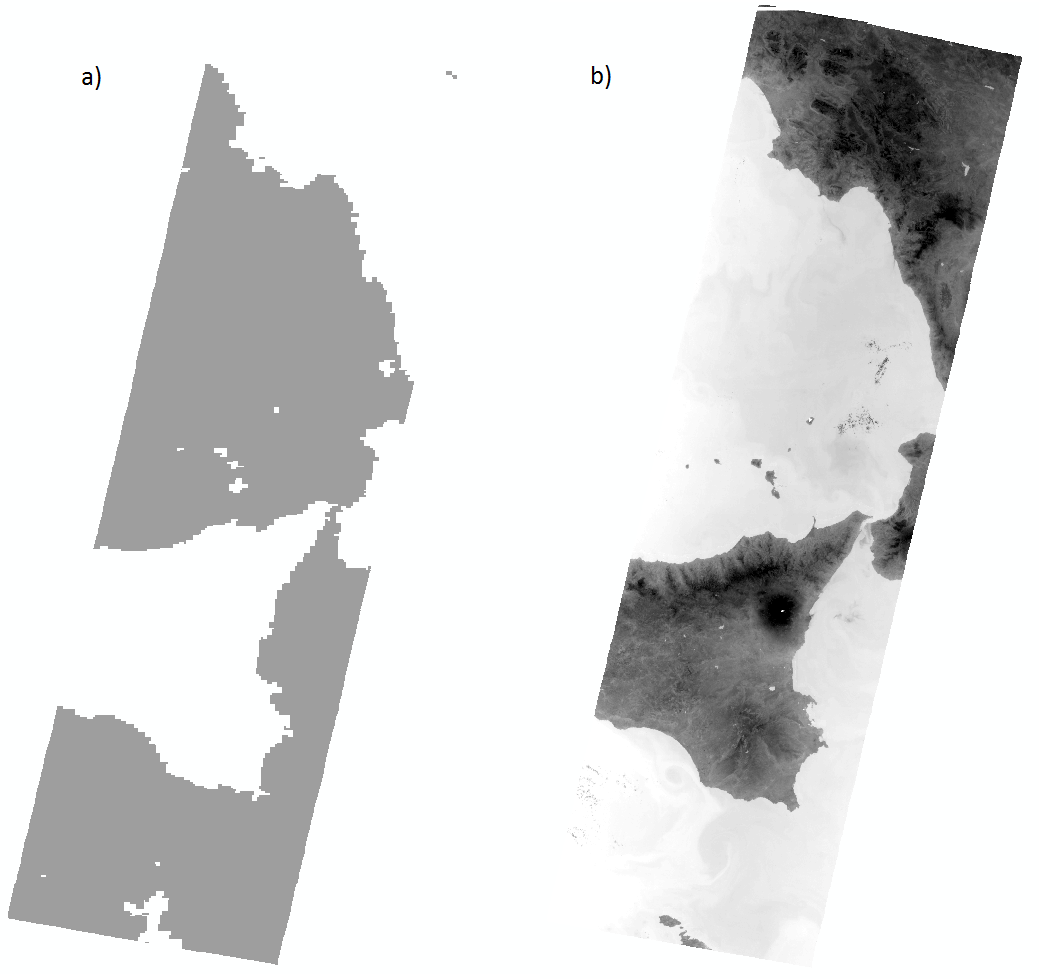
\includegraphics[width=0.6\textwidth]{SST.png}
\caption{a) MODIS SST. b) MITIP temperature product: surface temperature map in MIR band}
\label{fig:SST}
\end {figure}

\begin{figure}[!htbp]
\centering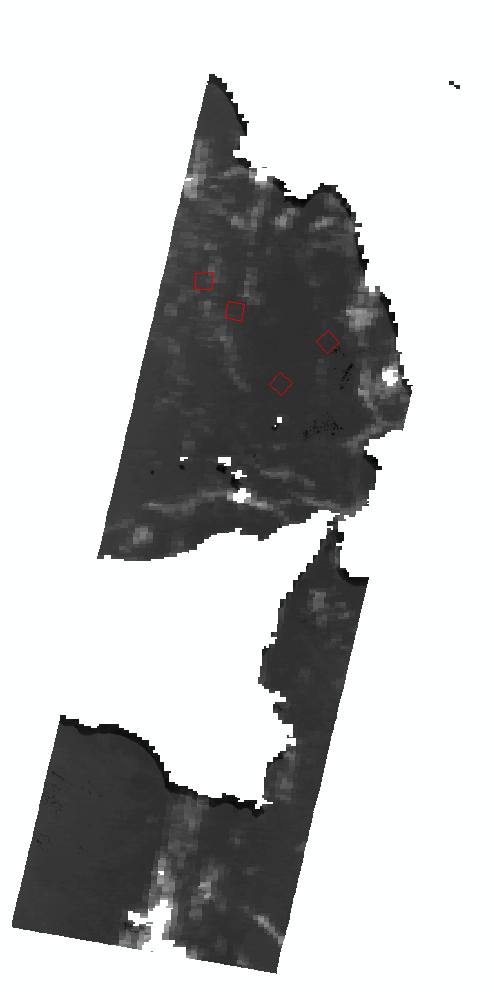
\includegraphics[width=0.4\textwidth]{differences.png}
\caption{Difference map between MODIS SST and MITIP surface temperature in MIR band}
\label{fig:Diff}
\end{figure}

\begin{figure}[!htbp]
\centering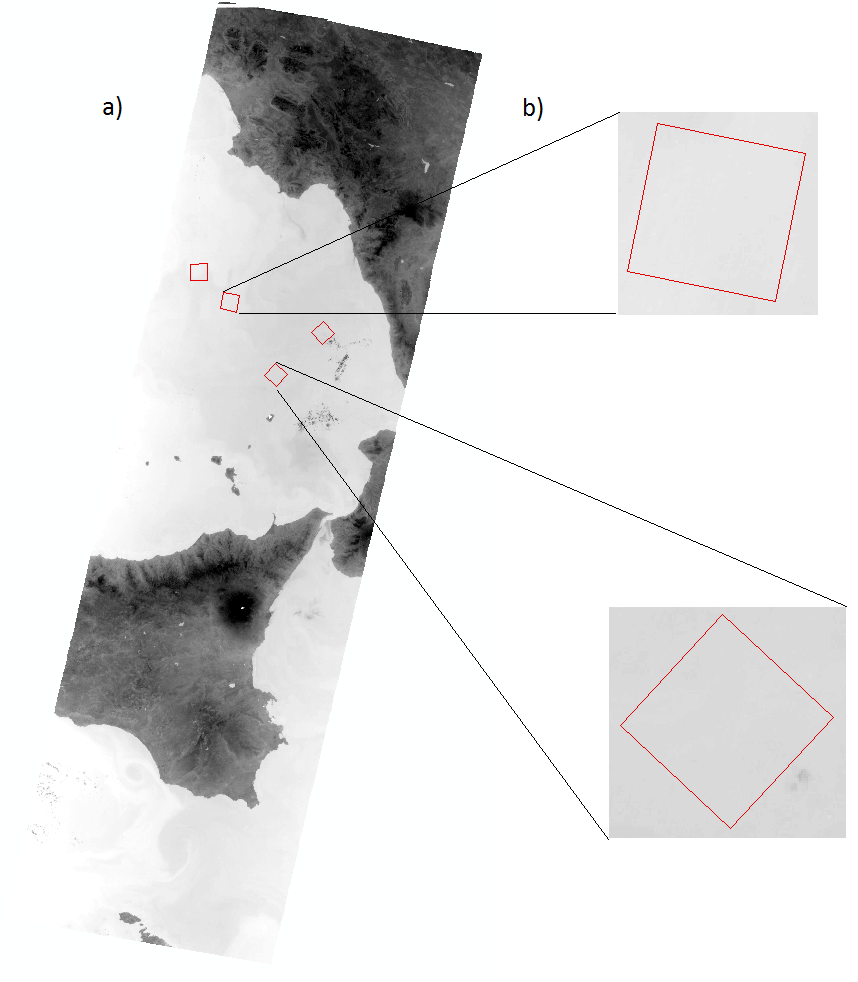
\includegraphics[width=0.6\textwidth]{selectedArea.png}
\caption{a) Selected sub-areas distribution over MITIP surface temperature in MIR band. b) Zoomed-in pictures of two sub-areas}
\label{fig:selectedArea}
\end{figure}

%-----------------------------------
%	SUBSECTION 2
%-----------------------------------

\subsection{Results comparison with MODIS SST and calibration}
Before doing the comparison between MODIS SST and MITIP surface temperature products, one problem needed to be solved is the choice of emissivity map. The emissivity map derived from ASTER Global Emissivity Database consists of 5 bands and there are two bands, namely band 11 with wavelength 8.6 $\mu$m and band 12 with wavelength 9.1 $\mu$m fall in TET-1 imagery's TIR band with spectral range 8.5 $\mu$m to 9.3 $\mu$m \parencite{Reference306}. So there comes a problem that which band of the emissivity maps should be used. This problem will be considered under different circumstances.\\

\noindent Since the emissivities of water body in these two bands are very close, 0.984  and 0.985 respectively, the effects of the different emissivities can be neglected when the results from MITIP are compared with MODIS SST as shown Figure \ref{fig:tem_diff_emi1}.\\

\begin{figure}[!htbp]
\centering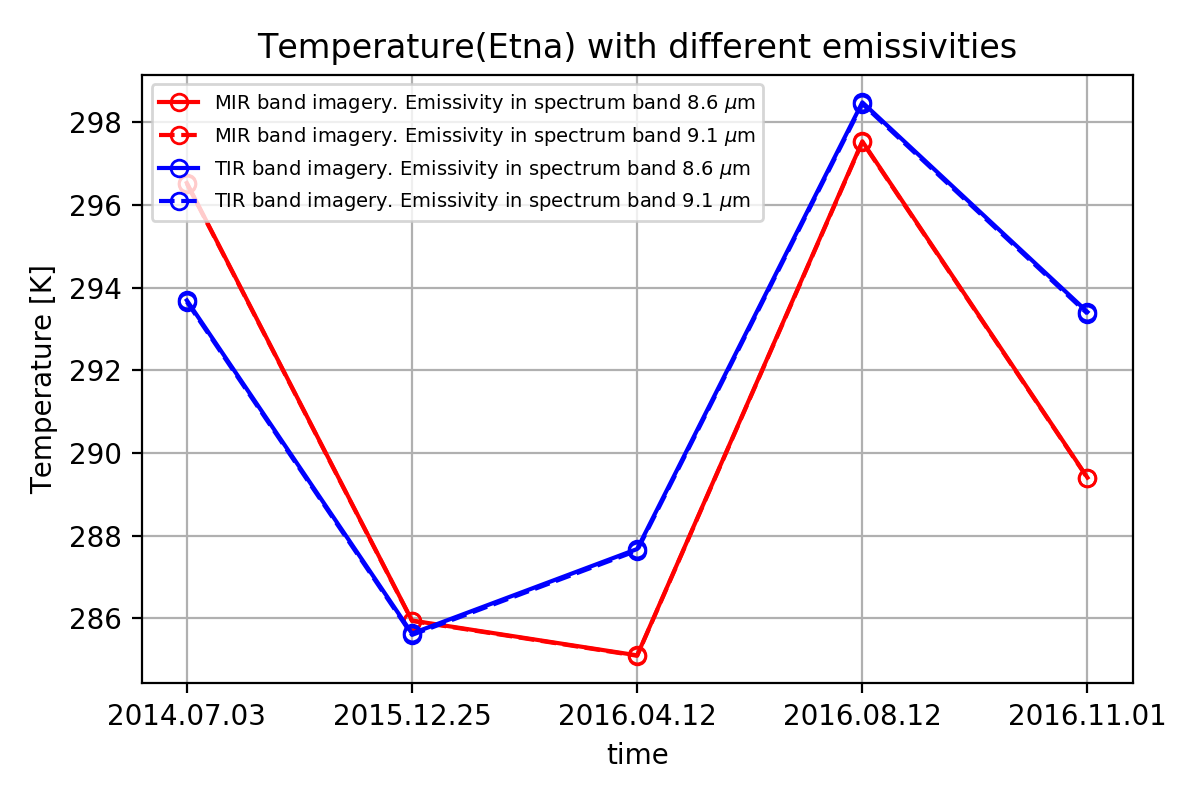
\includegraphics[width=0.8\textwidth]{diff_emi1.png}
\caption{Mean temperature of all sub-areas in Etna scenes with different emissivities}
\label{fig:tem_diff_emi1}
\end{figure}

\begin{figure}[!htbp]
\centering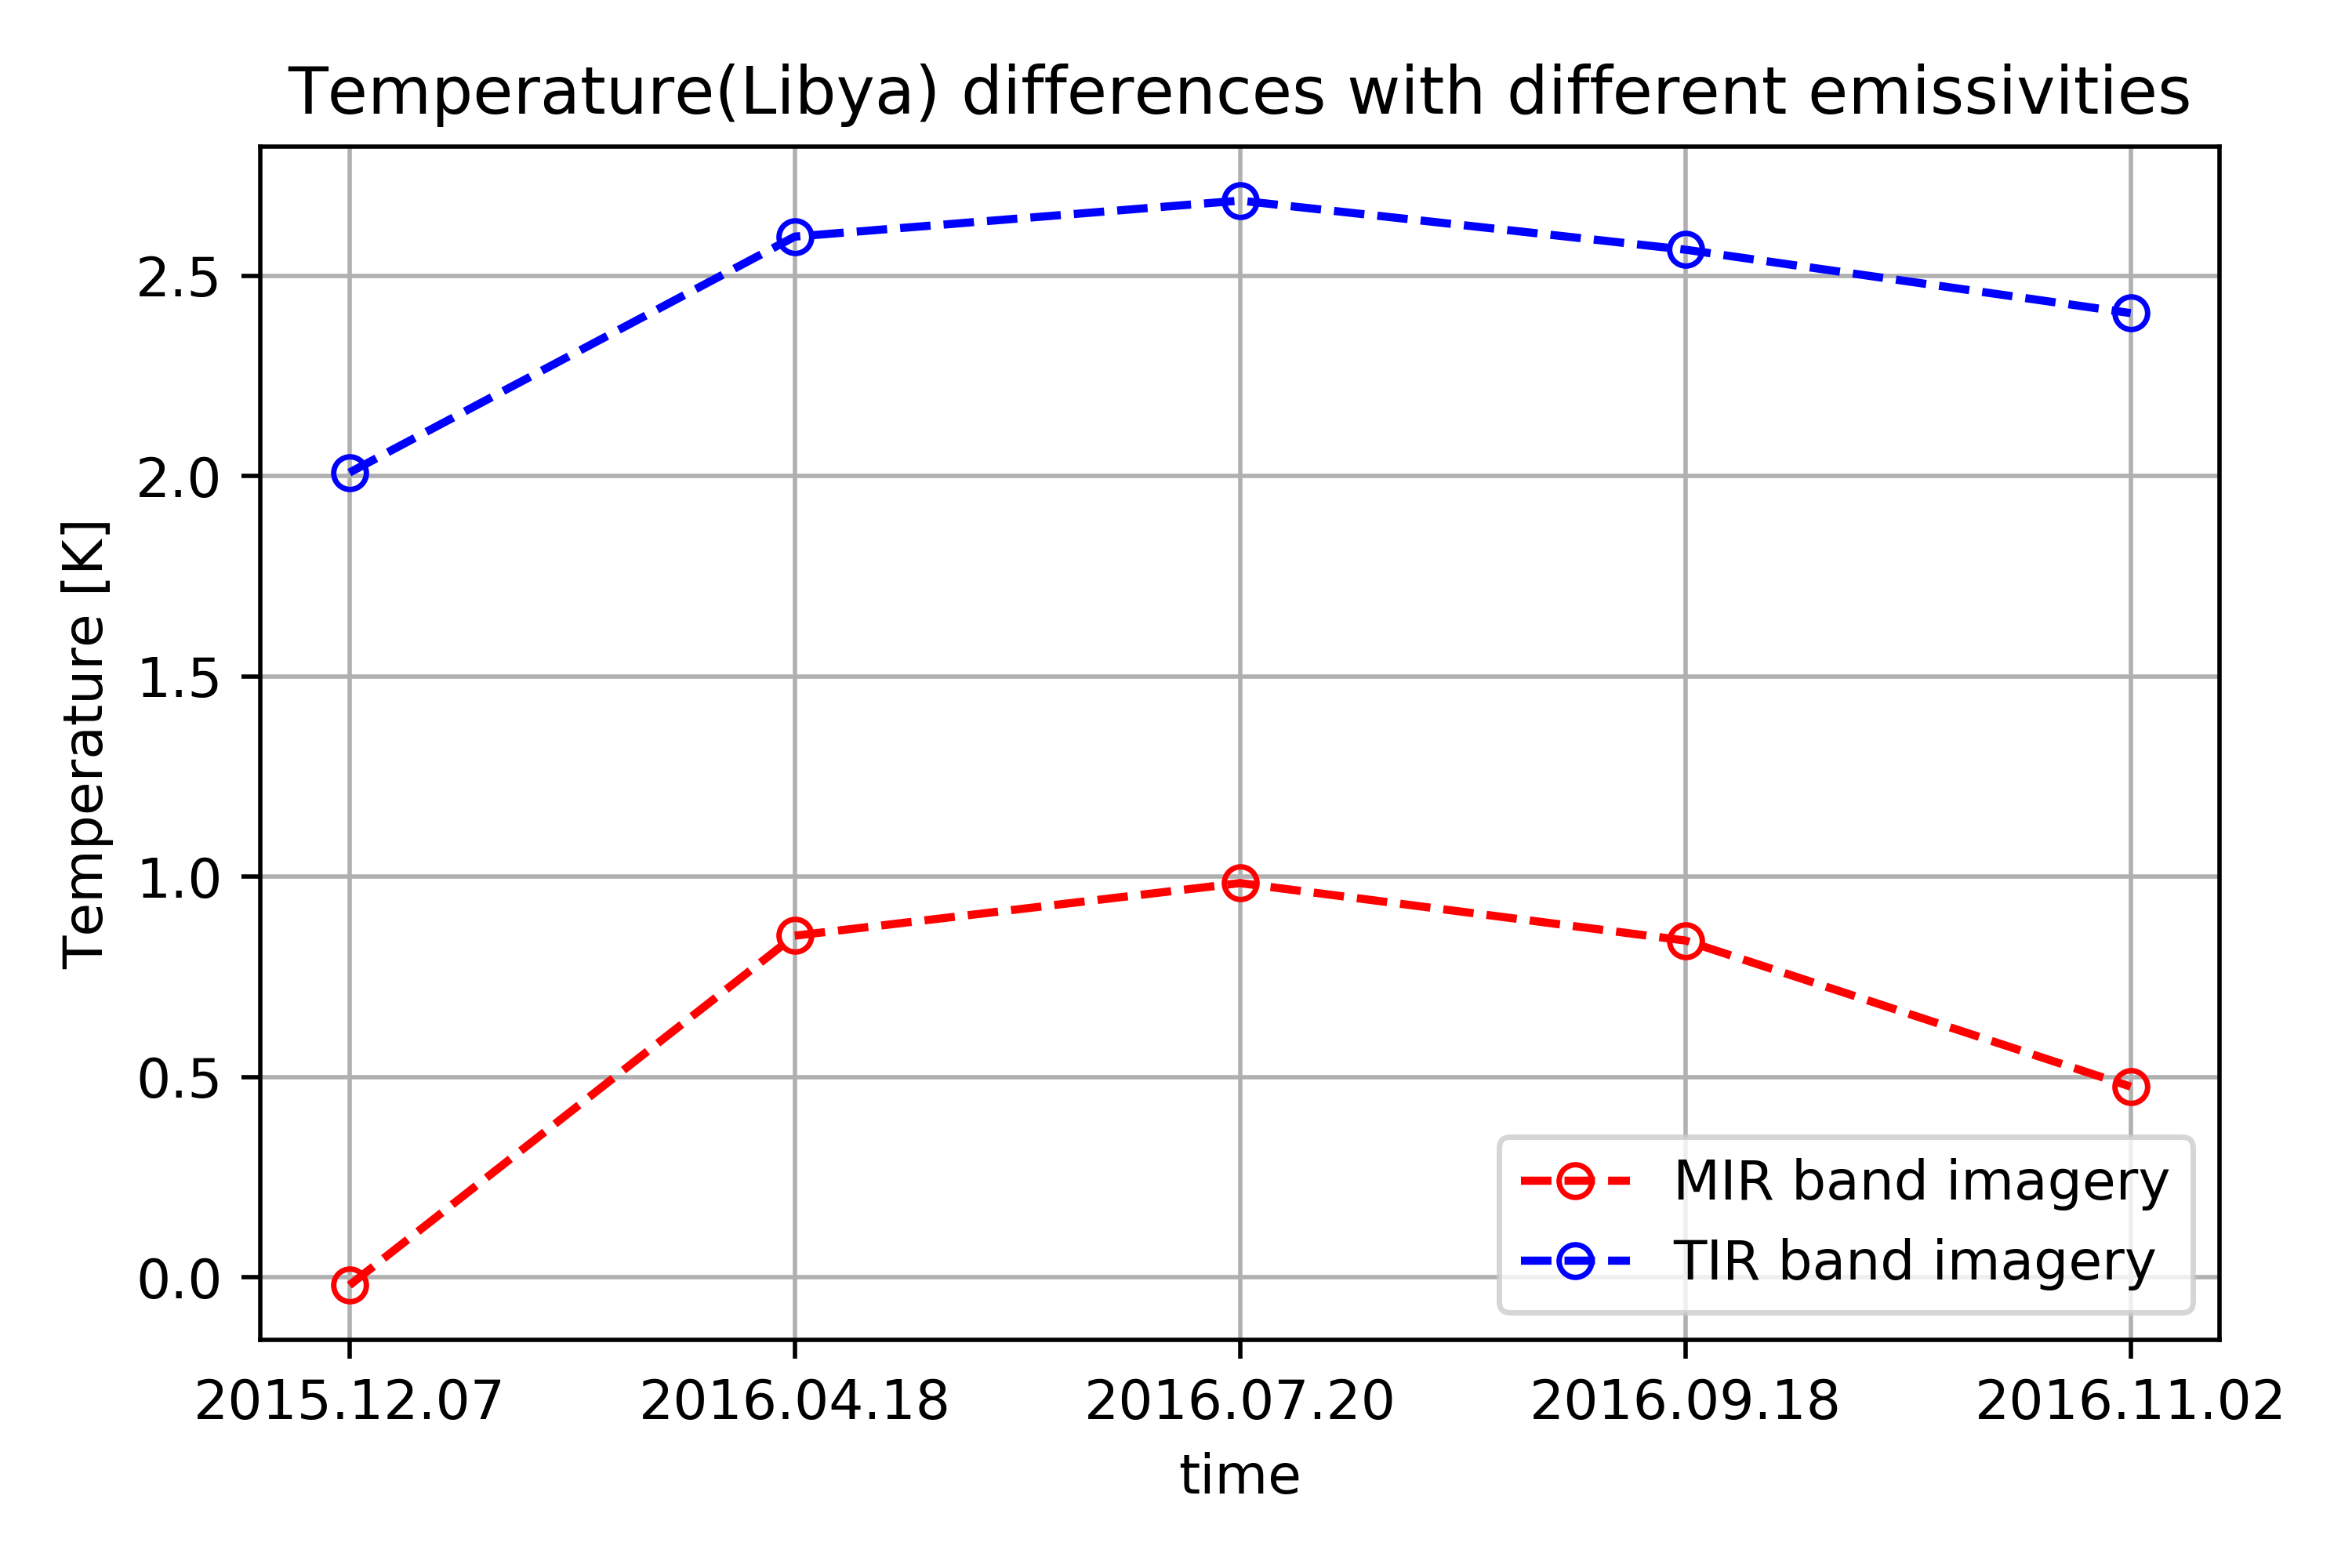
\includegraphics[width=0.8\textwidth]{diff_emi2.png}
\caption{Differences of temperatures resulted from different emissivities(Etna)}
\label{fig:tem_diff_emi2}
\end{figure}

\noindent From Figure \ref{fig:tem_diff_emi2} we can see that the temperature differences resulted from different emissivities in MIR band imagries are within the range (0.010K, 0.018K). The temperature differences resulted from different emissivities in TIR band imagries are within the range (0.032K, 0.040K). Both of them are so small that can be neglected in the context of the area of interest (AOI) is water. Here the emissivity map in band 8.6 $\mu$m is used.\\

\noindent Firstly, the surface temperature maps from MITIP are compare with MODIS SST according to the steps states in Section 4.1. The Figure \ref{fig:tem_com} shows that the surface temperatures derived by MITIP are lower than those of the MODIS SST on both the MIR band and TIR band. To adjust these differences, TOA radiances, which are the pixel values of the original TET-1 imageries, need to be calibrated.\\

\begin{figure}[!htbp]
\centering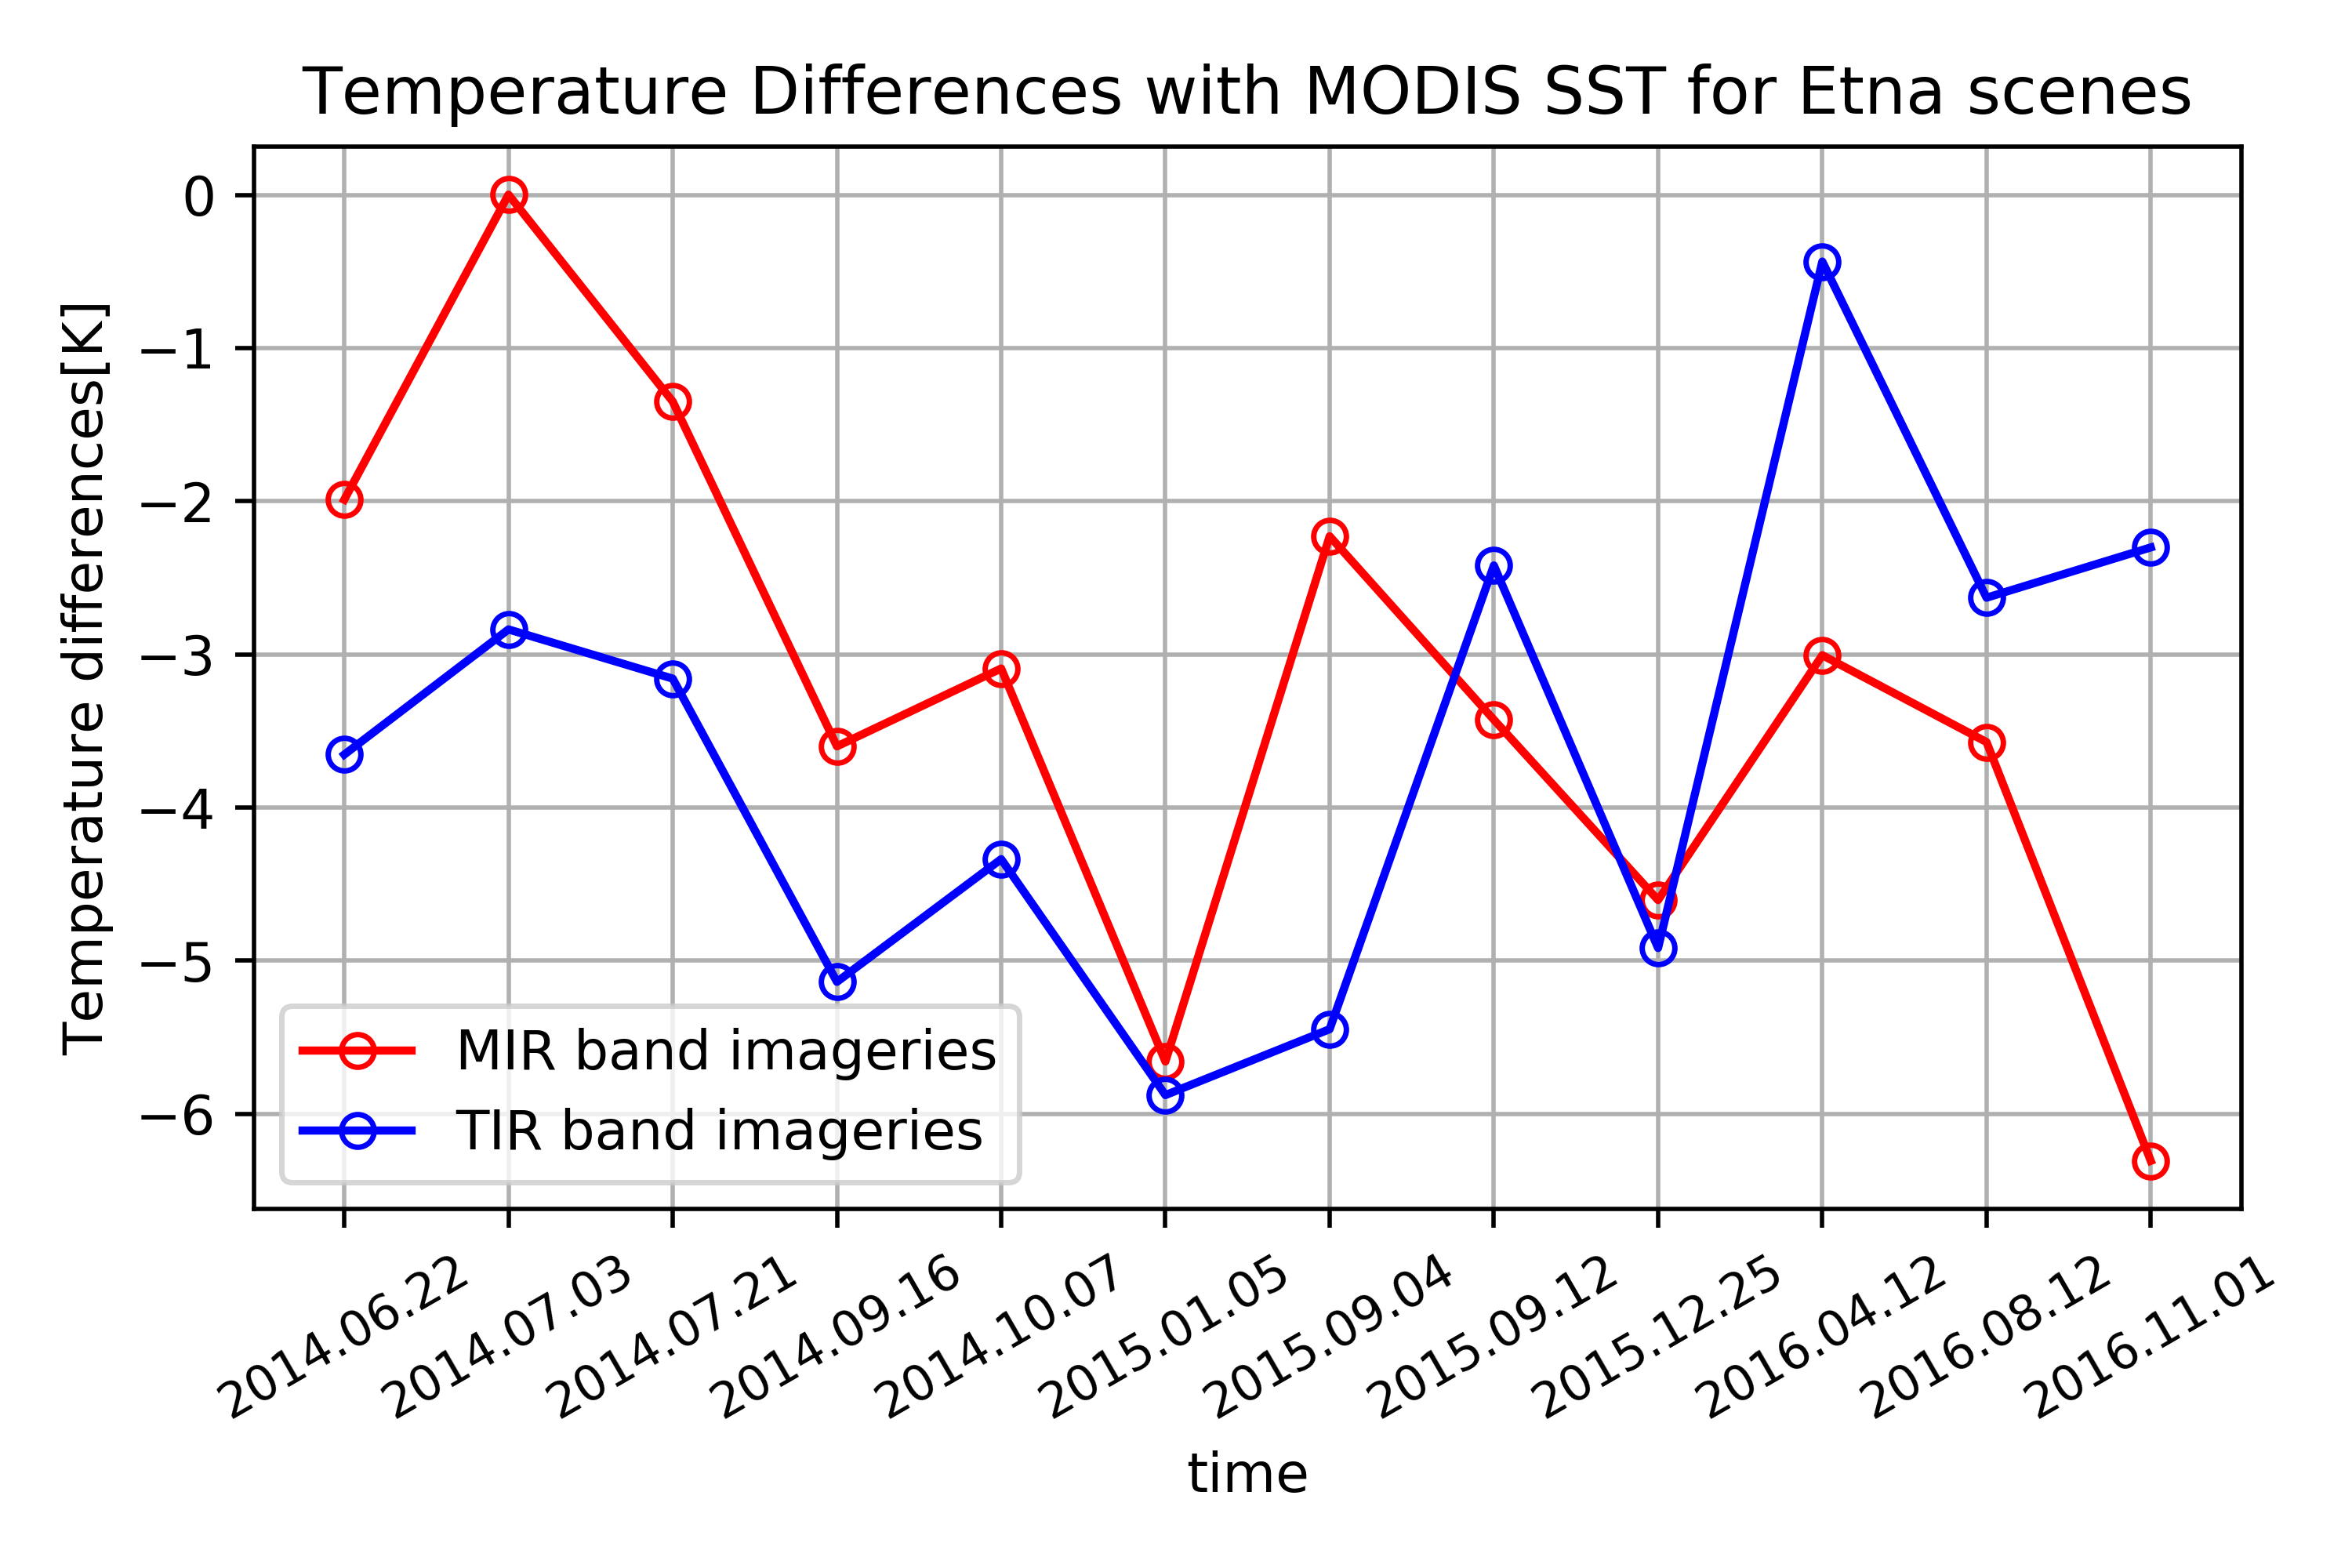
\includegraphics[width = 0.8\textwidth]{tem_com.png}
\caption{Temperature differences between the temperature maps from MITIP and MODIS SST for Etna scenes}
\label{fig:tem_com}
\end{figure}

\noindent As a result, the MITIP method adds two input keywords \emph{sc1} and \emph{sc2}, which stand for scale factor for the TET-1 MIR and TIR band imageries respectively, to calibrate the TOA radiances. Since the temperatures derived from MITIP are lower than the MODIS SST, the TOA radiances of the TET-1 imagery should be increased. As a result, five scale factors, 1.00 which means original TOA radiances, 1.05 which means increasing the TOA radiances by 5\%, 1.10, 1.15 and 1.20, are selected to calibrate the TET-1 MIR and TIR band respectively.\\

\noindent In order to see detailedly how the scale factor will affect the pixel values of the results of MITIP, histograms of sub-areas of TET-1 MIR band temperature map are investigated and compared with the histograms of the same areas of MODIS SST. The histograms of each sub-area with different scale factors are showed in Figure \ref{fig:hist_rect_all}. Here we use the Etna scene of the date 2014.06.22, which is the first scene we have for the Etna.\\

\begin{figure}[!htbp]
\centering
\subfigure[Sub-area 1 with scale factor 1.00]{
\label{fig:hist_rect1_1}
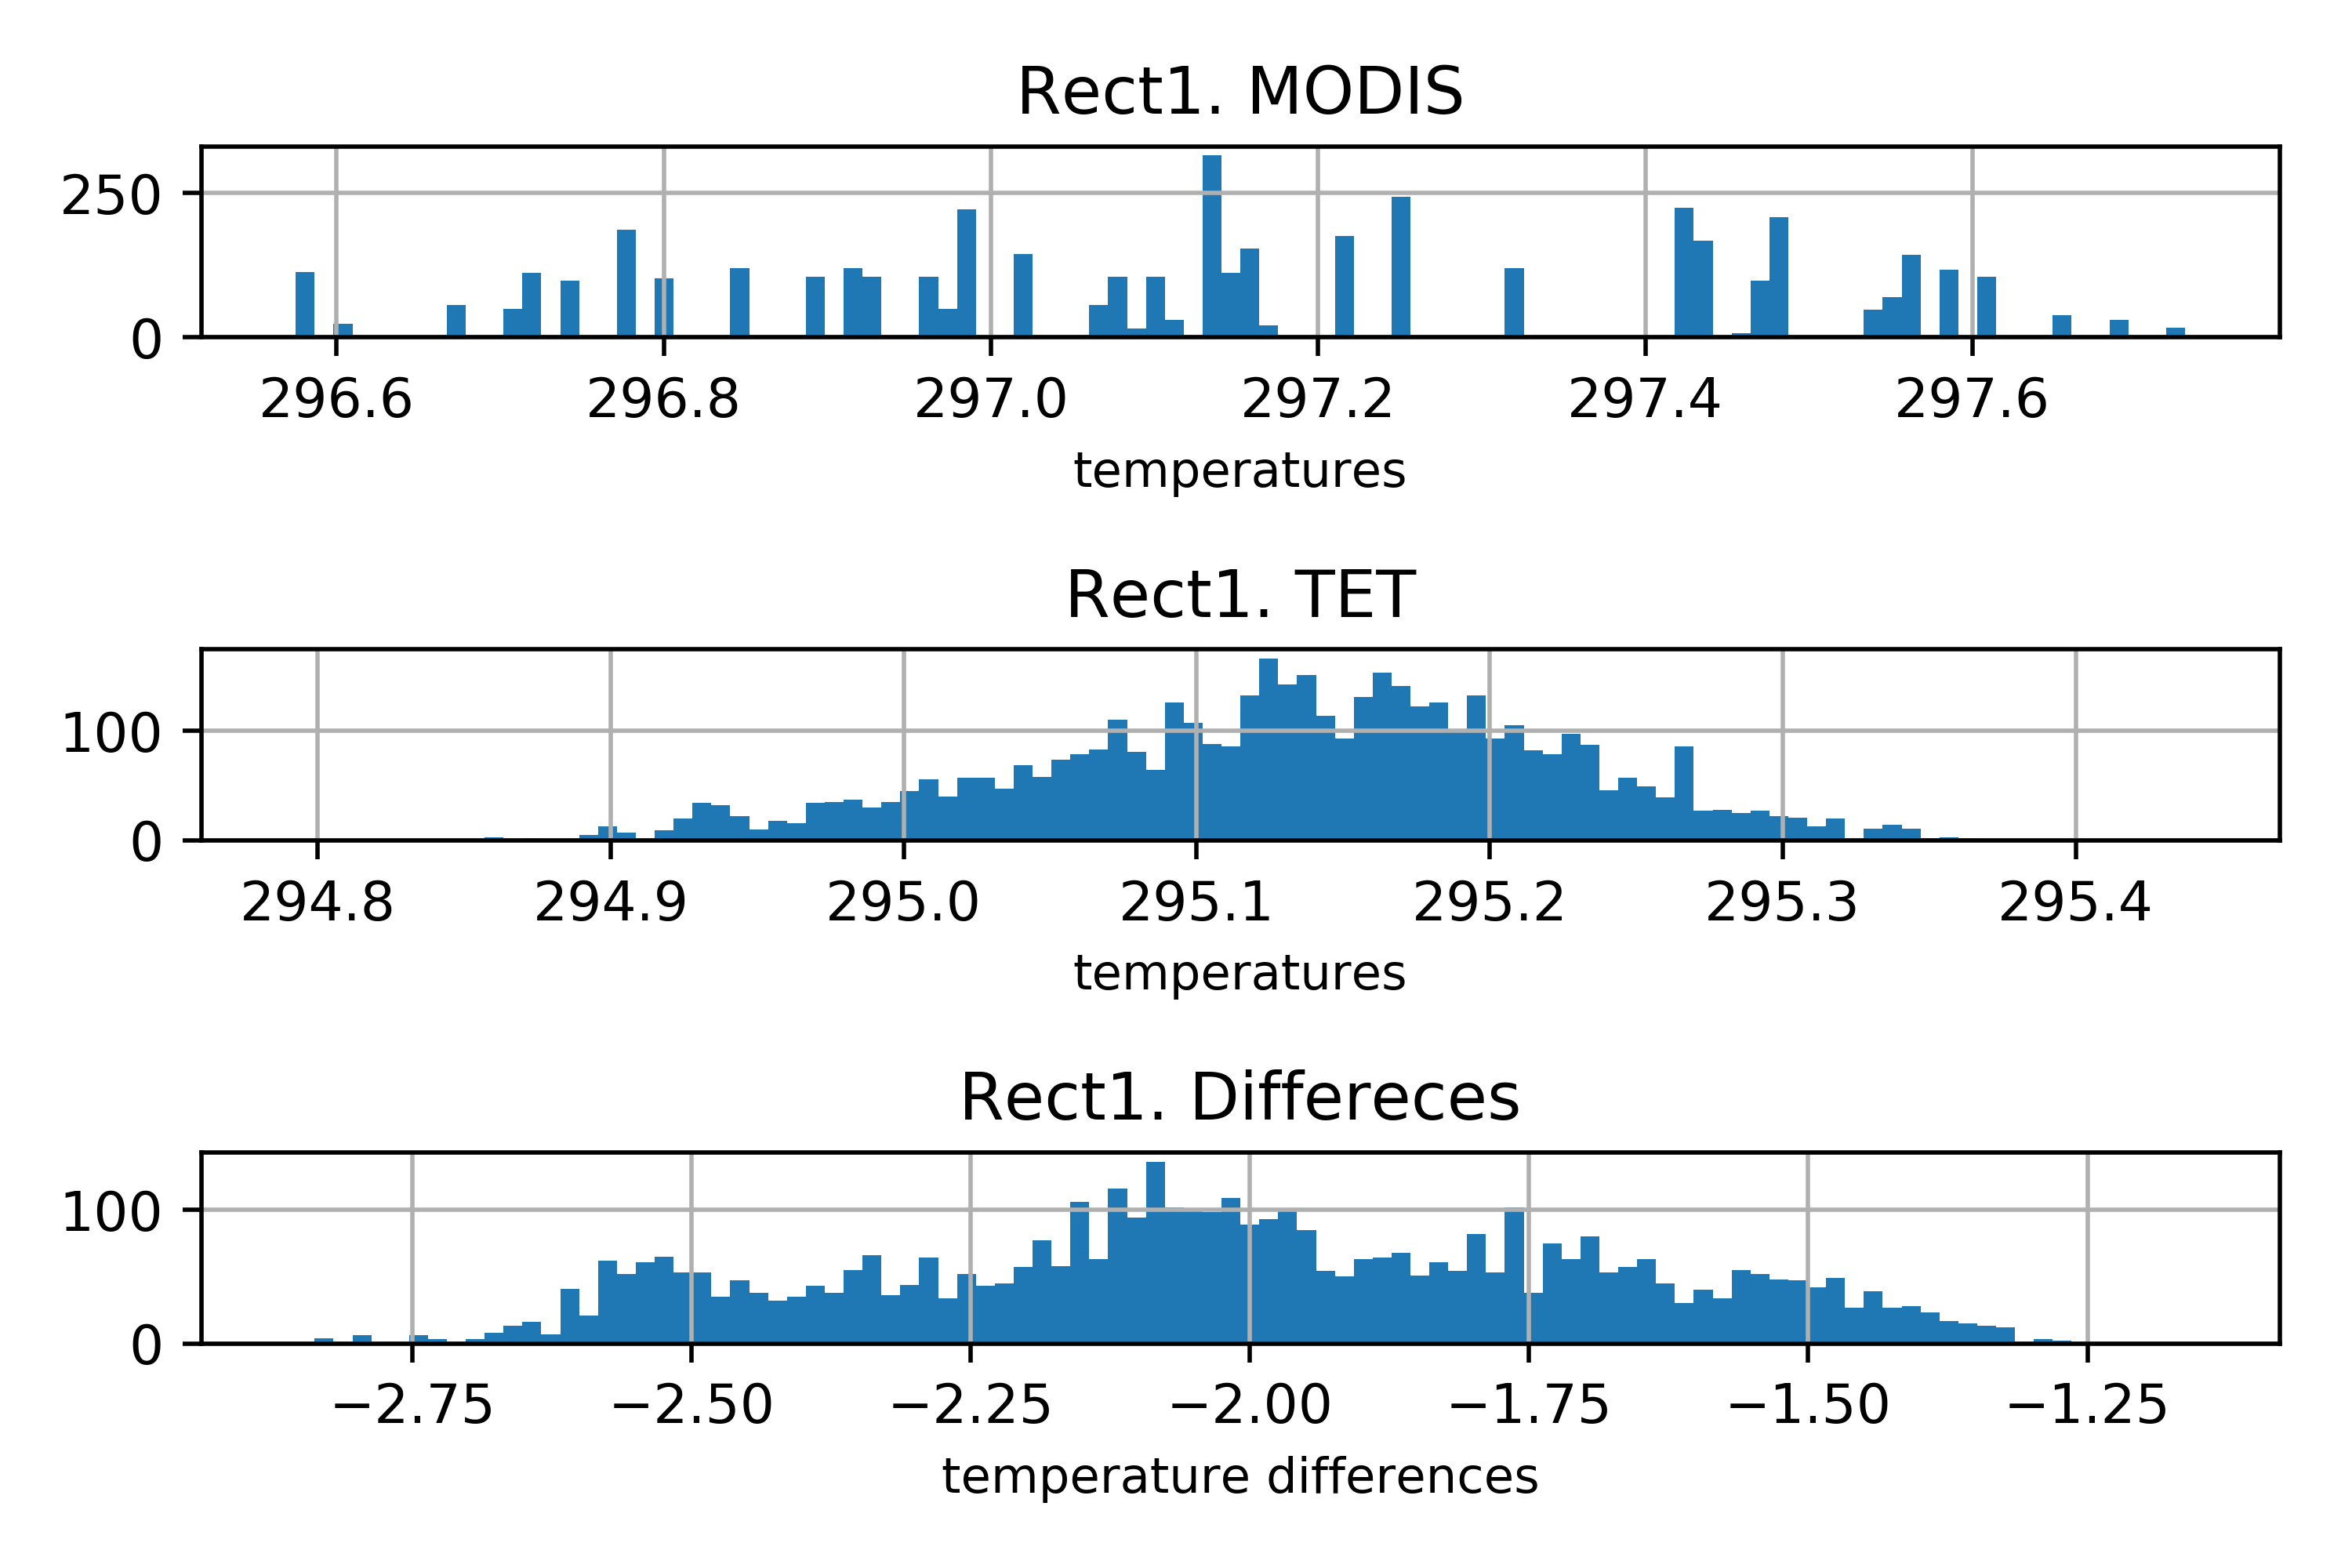
\includegraphics[width = 0.48\linewidth]{rect1_sc100.png}}
\vspace{0.1in}
\subfigure[Sub-area 1 with scale factor 1.10]{
\label{fig:hist_rect1_2}
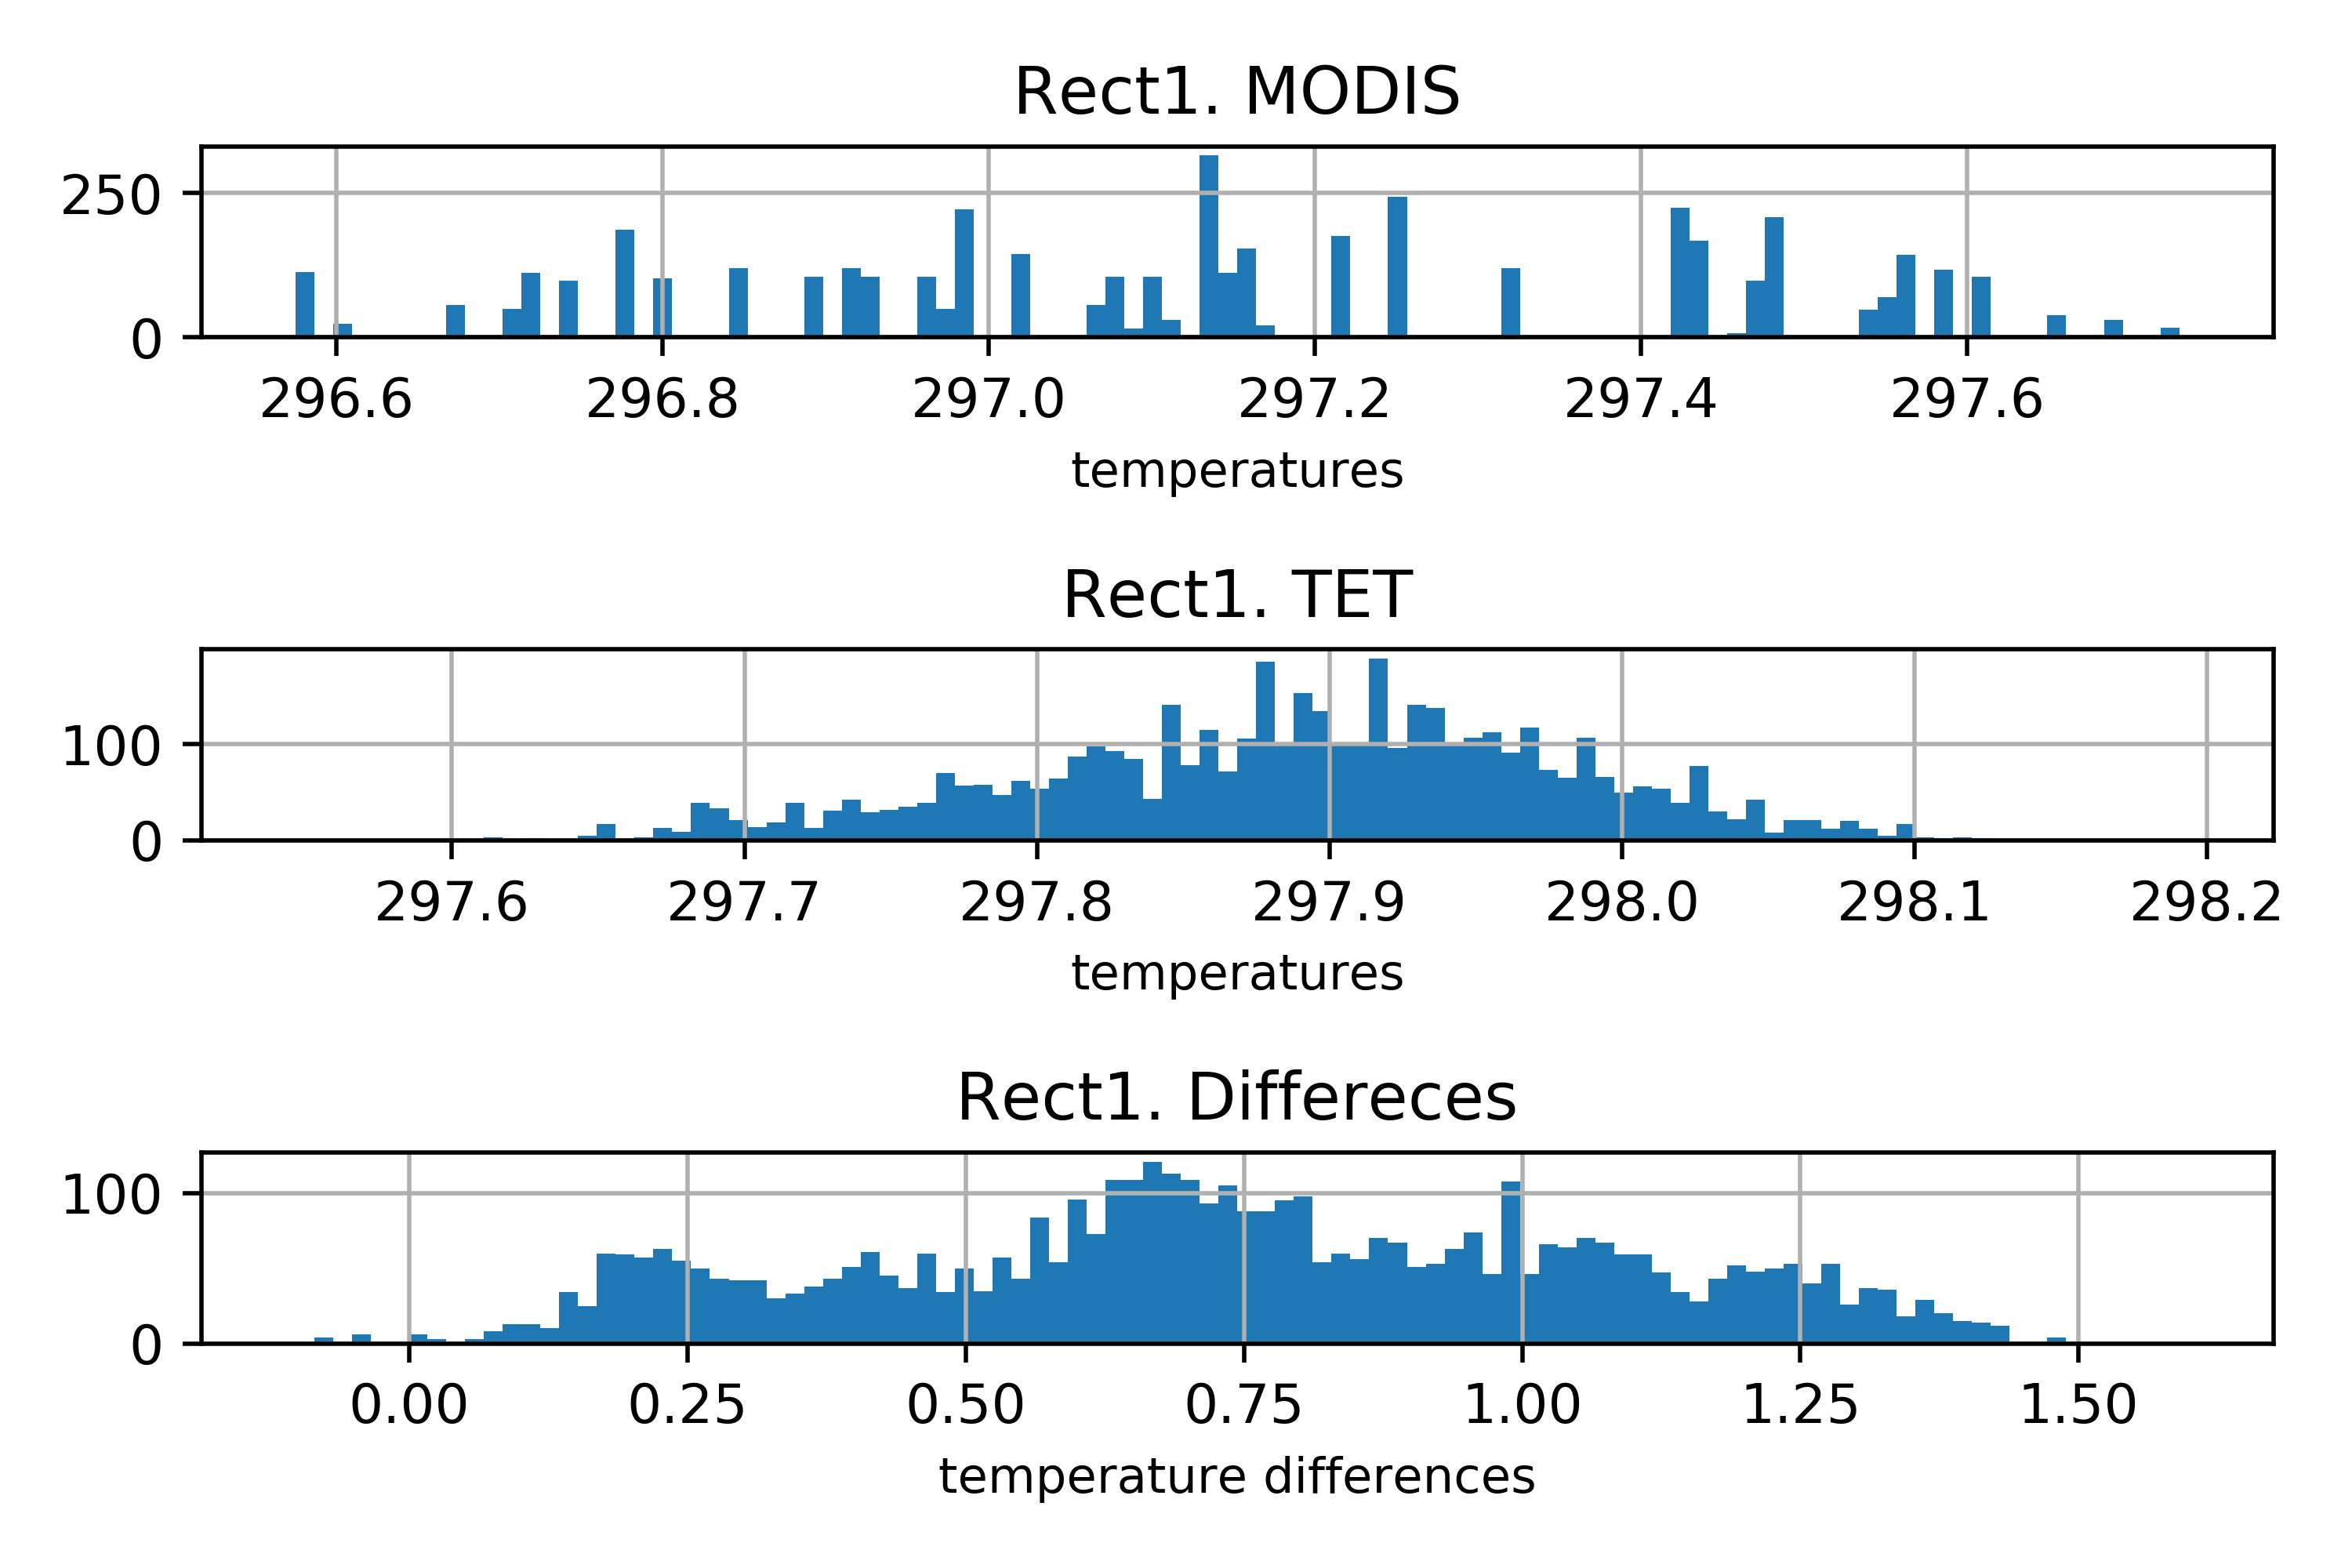
\includegraphics[width = 0.48\linewidth]{rect1_sc110.png}}

\hspace{0.5in}

\subfigure[Sub-area 2 with cale factor 1.00]{
\label{fig:hist_rect2_1}
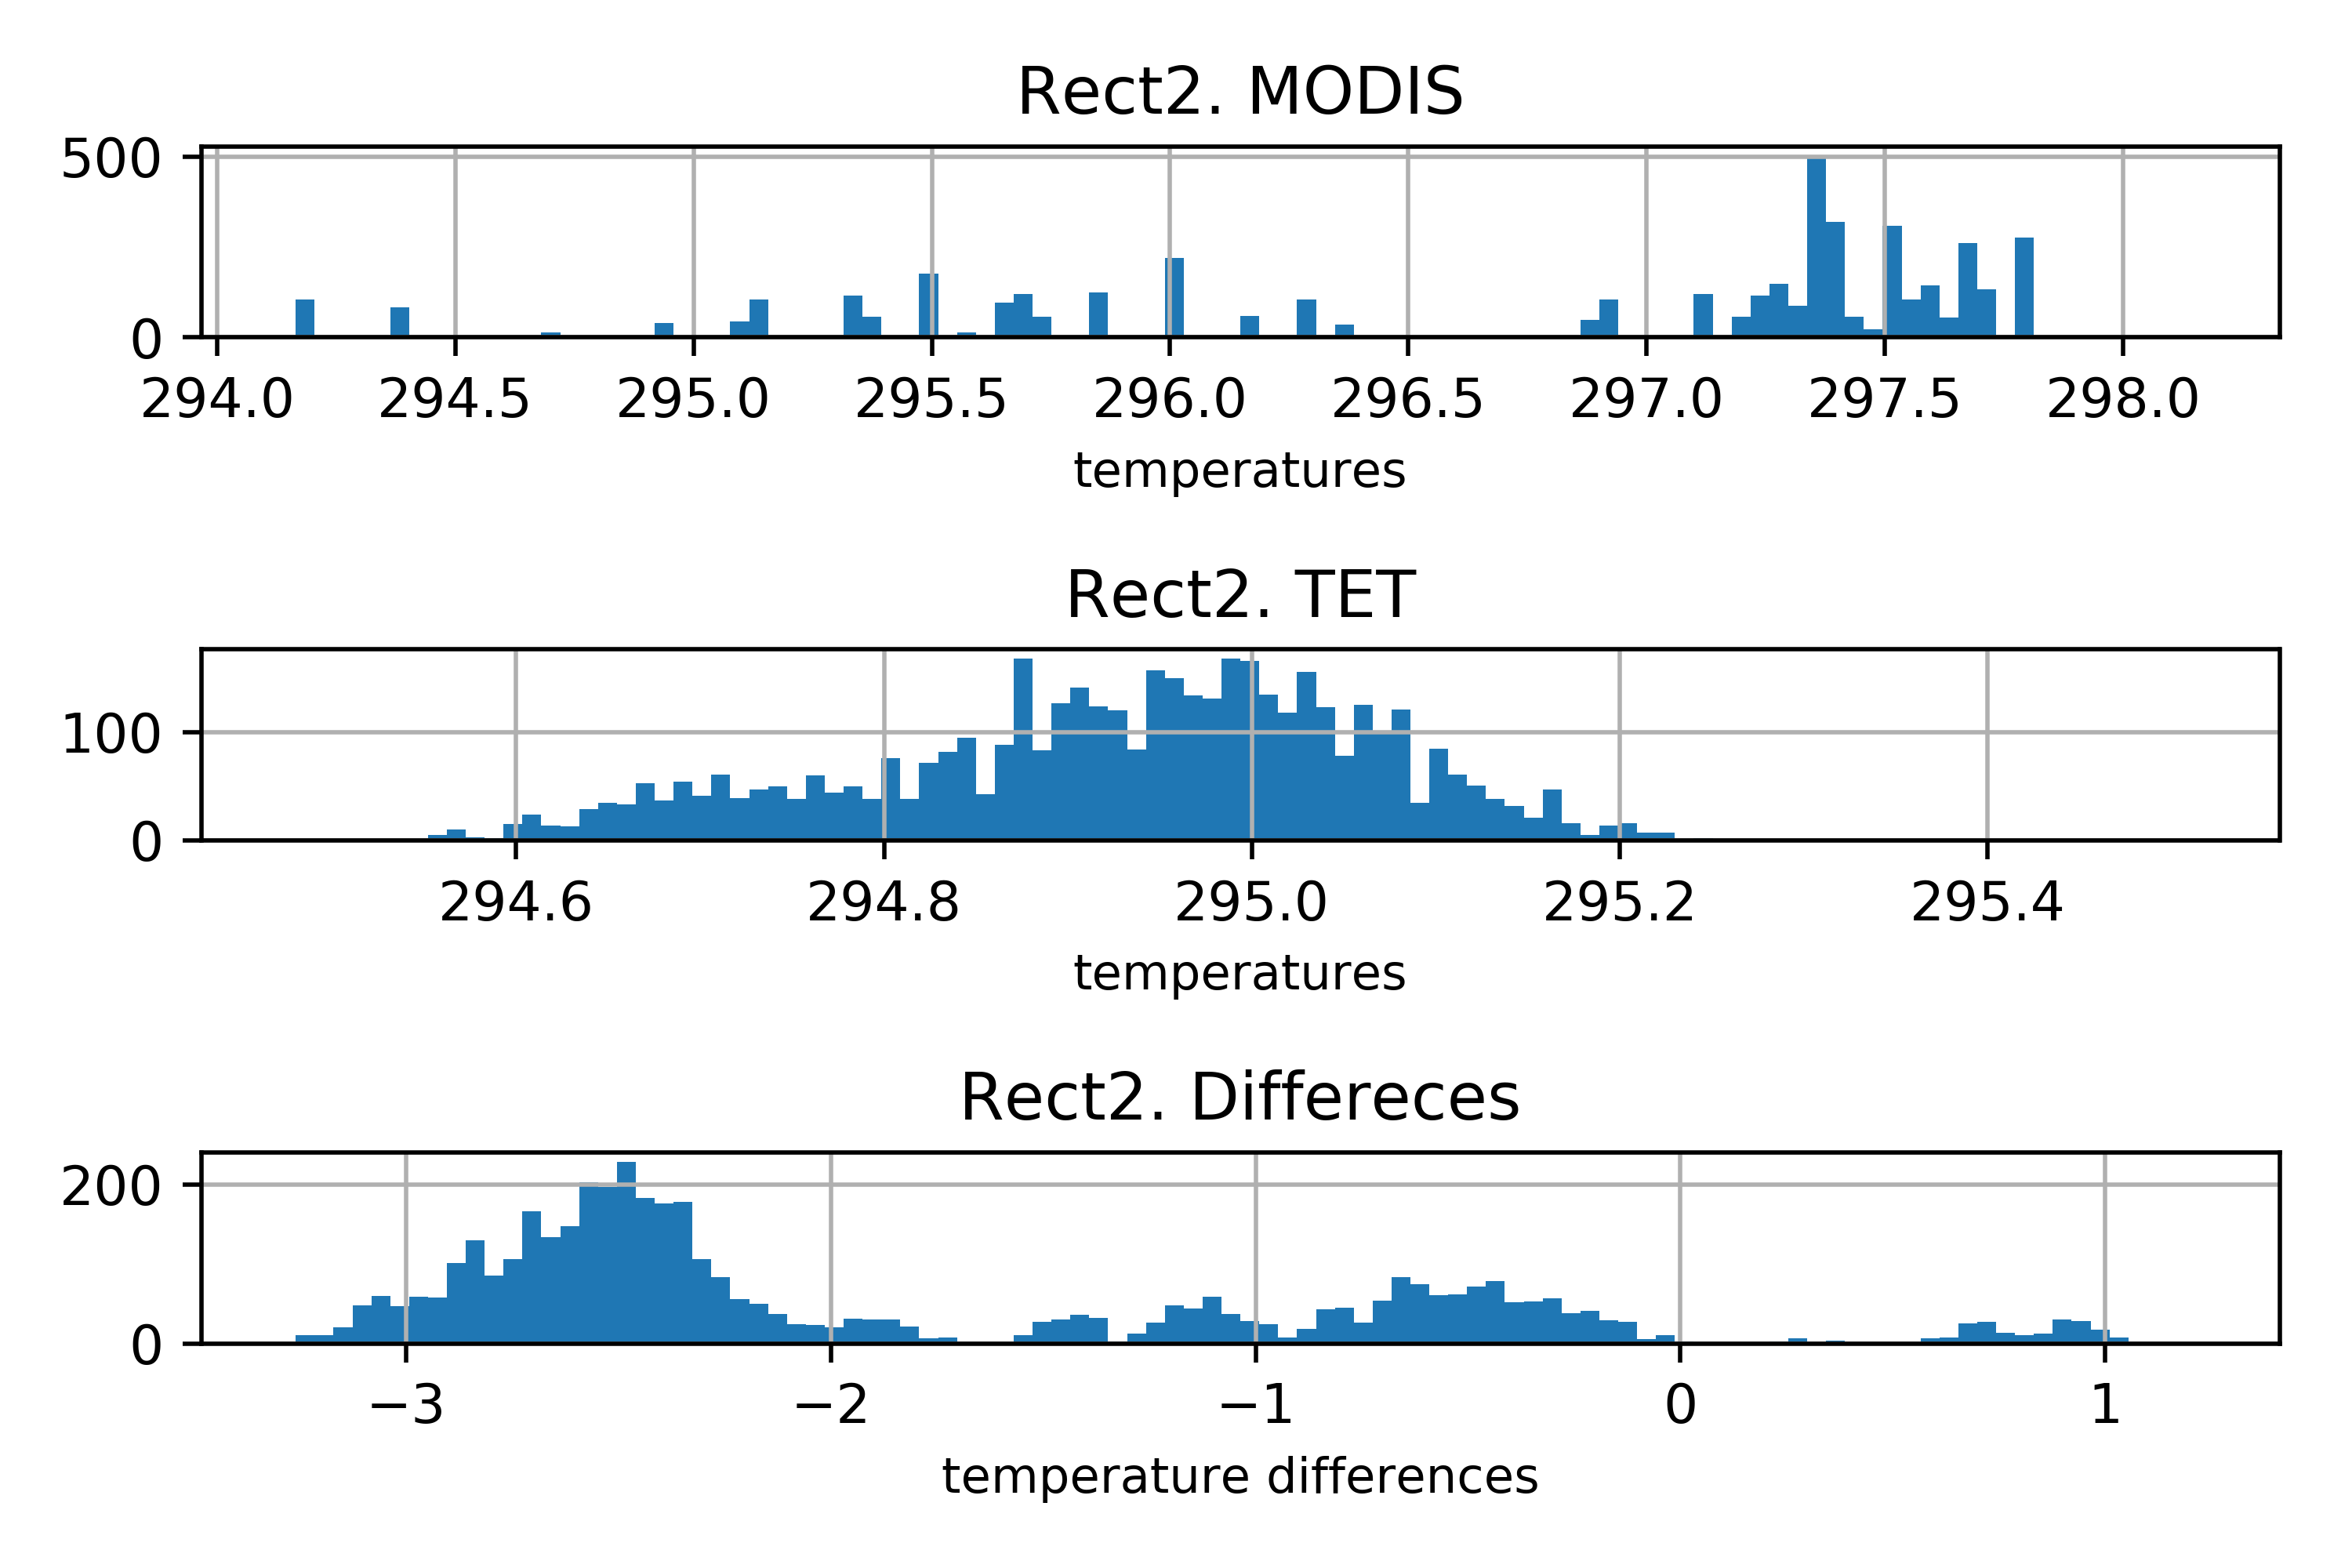
\includegraphics[width = 0.48\linewidth]{rect2_sc100.png}}
\vspace{0.1in}
\subfigure[Sub-area 2 with cale factor 1.10]{
\label{fig:hist_rect2_2}
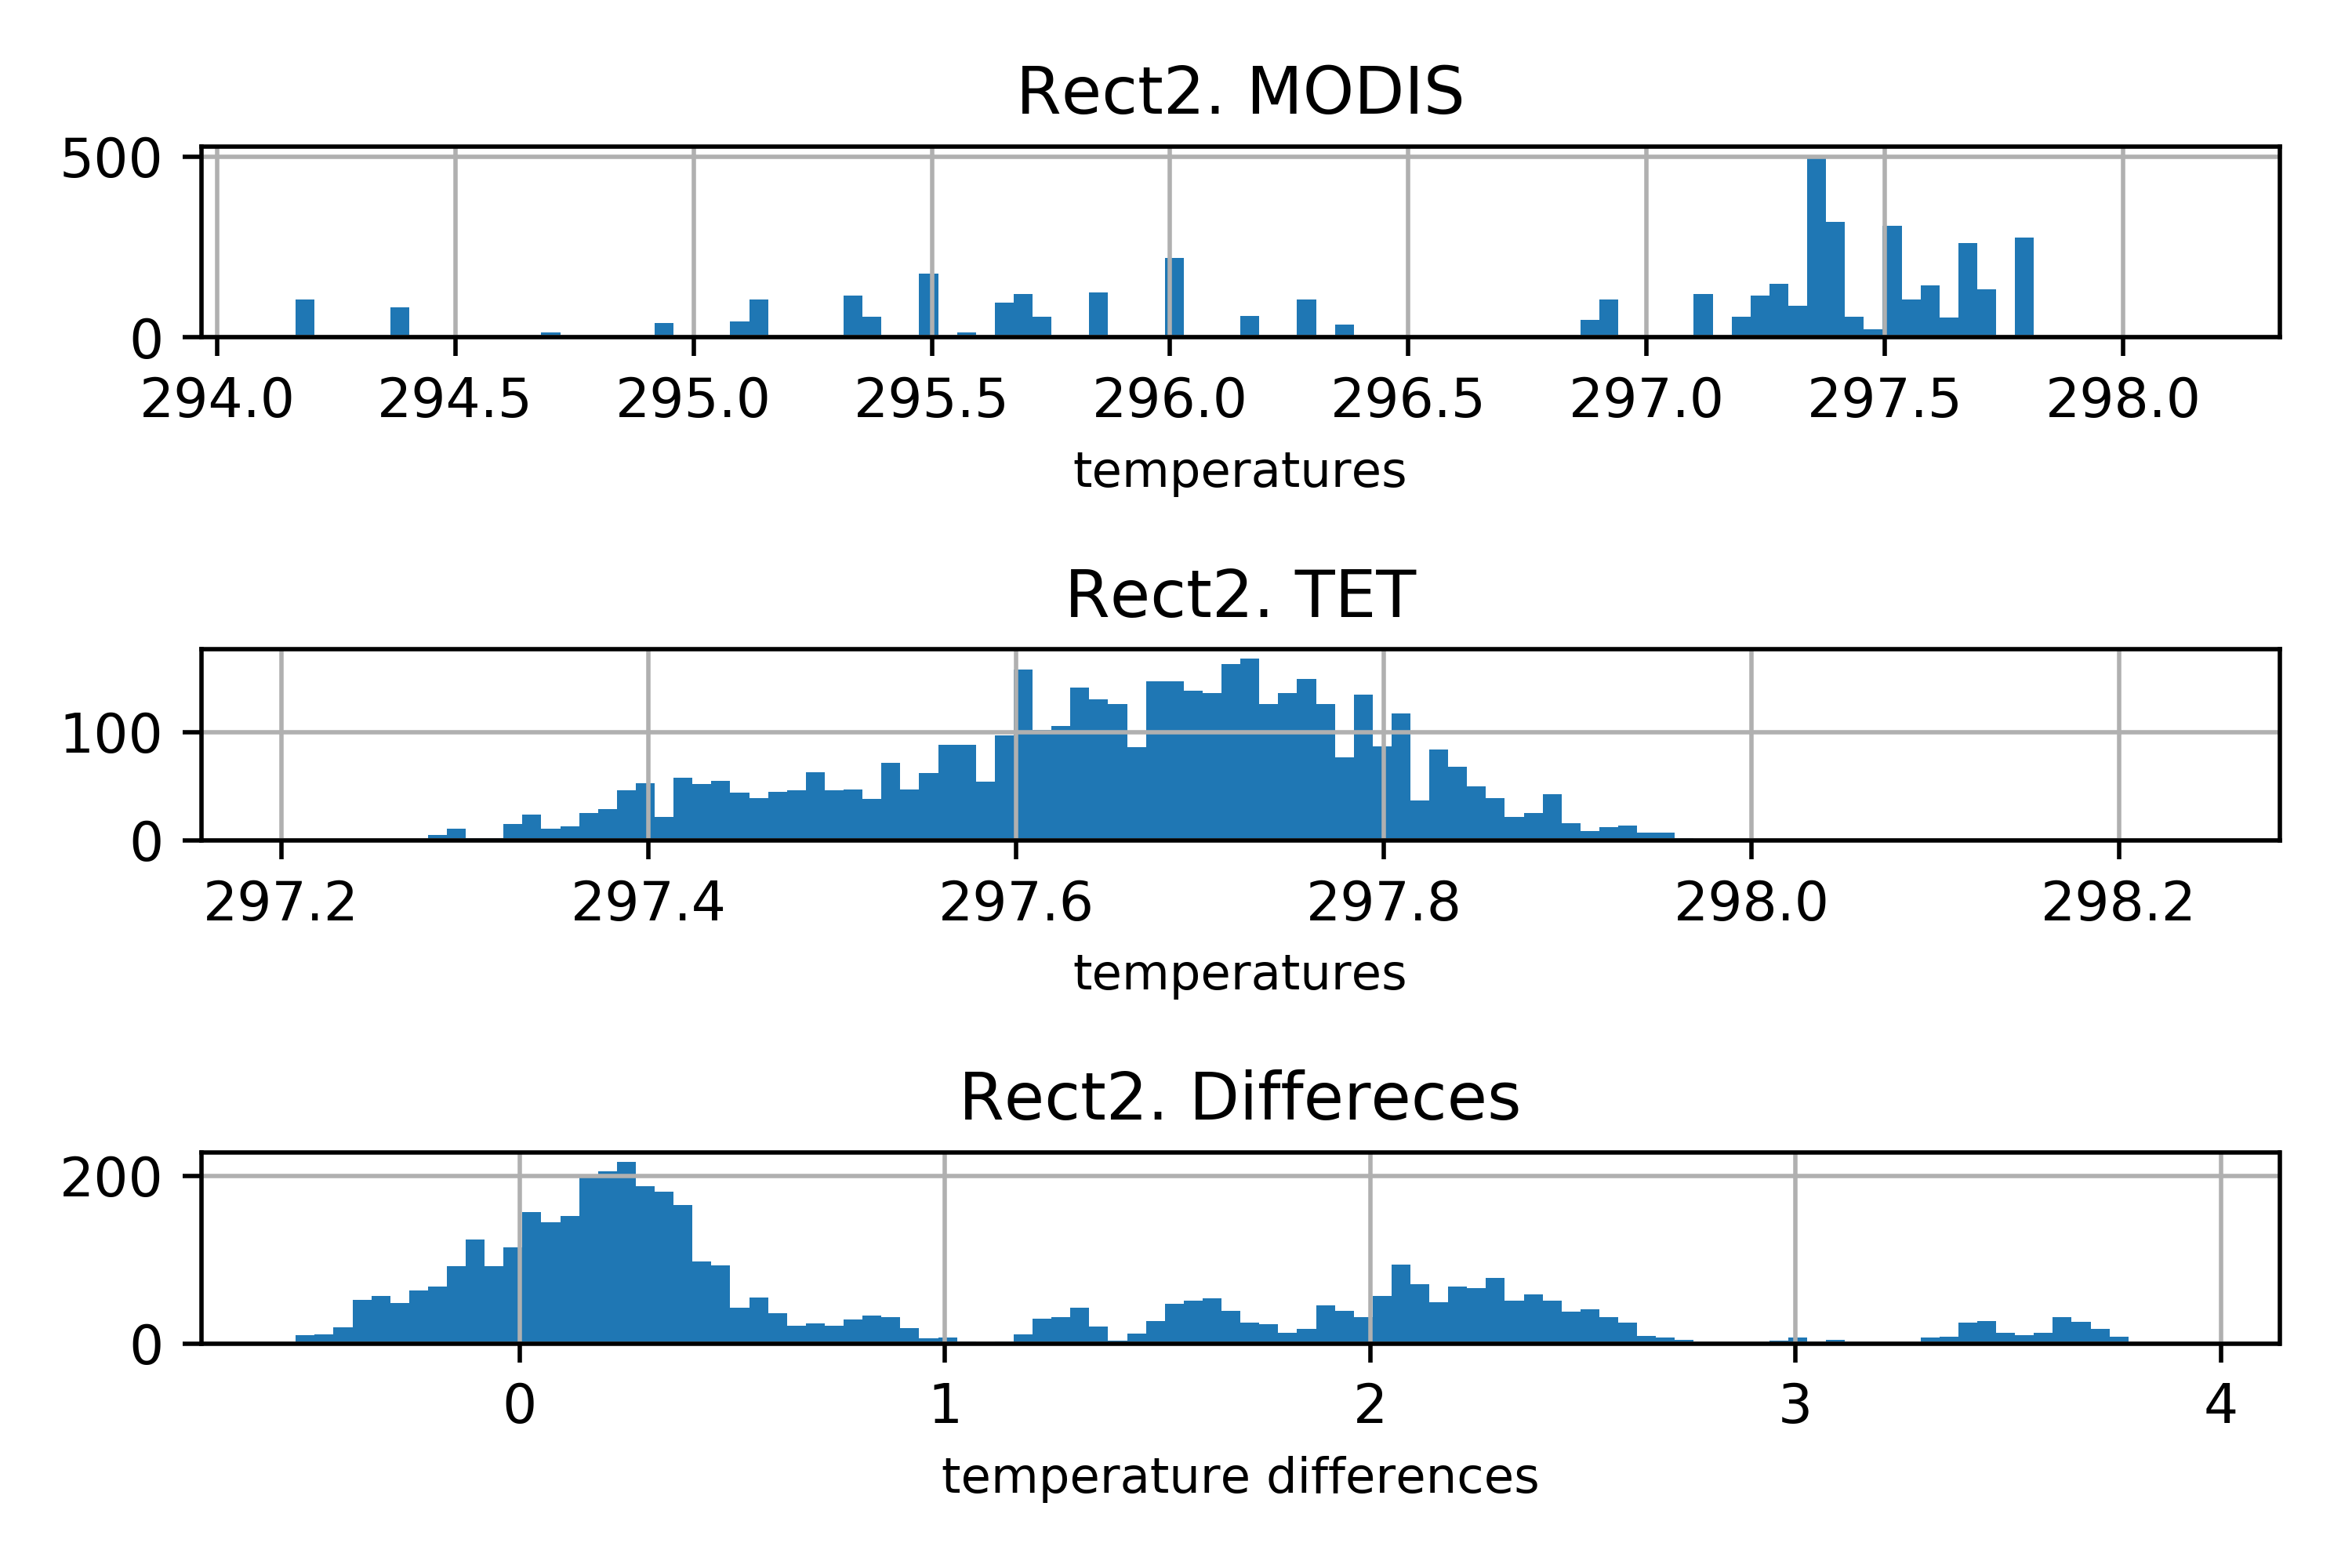
\includegraphics[width = 0.48\linewidth]{rect2_sc110.png}}

\hspace{0.5in}

\subfigure[Sub-area 3 with cale factor 1.00]{
\label{fig:hist_rect3_1}
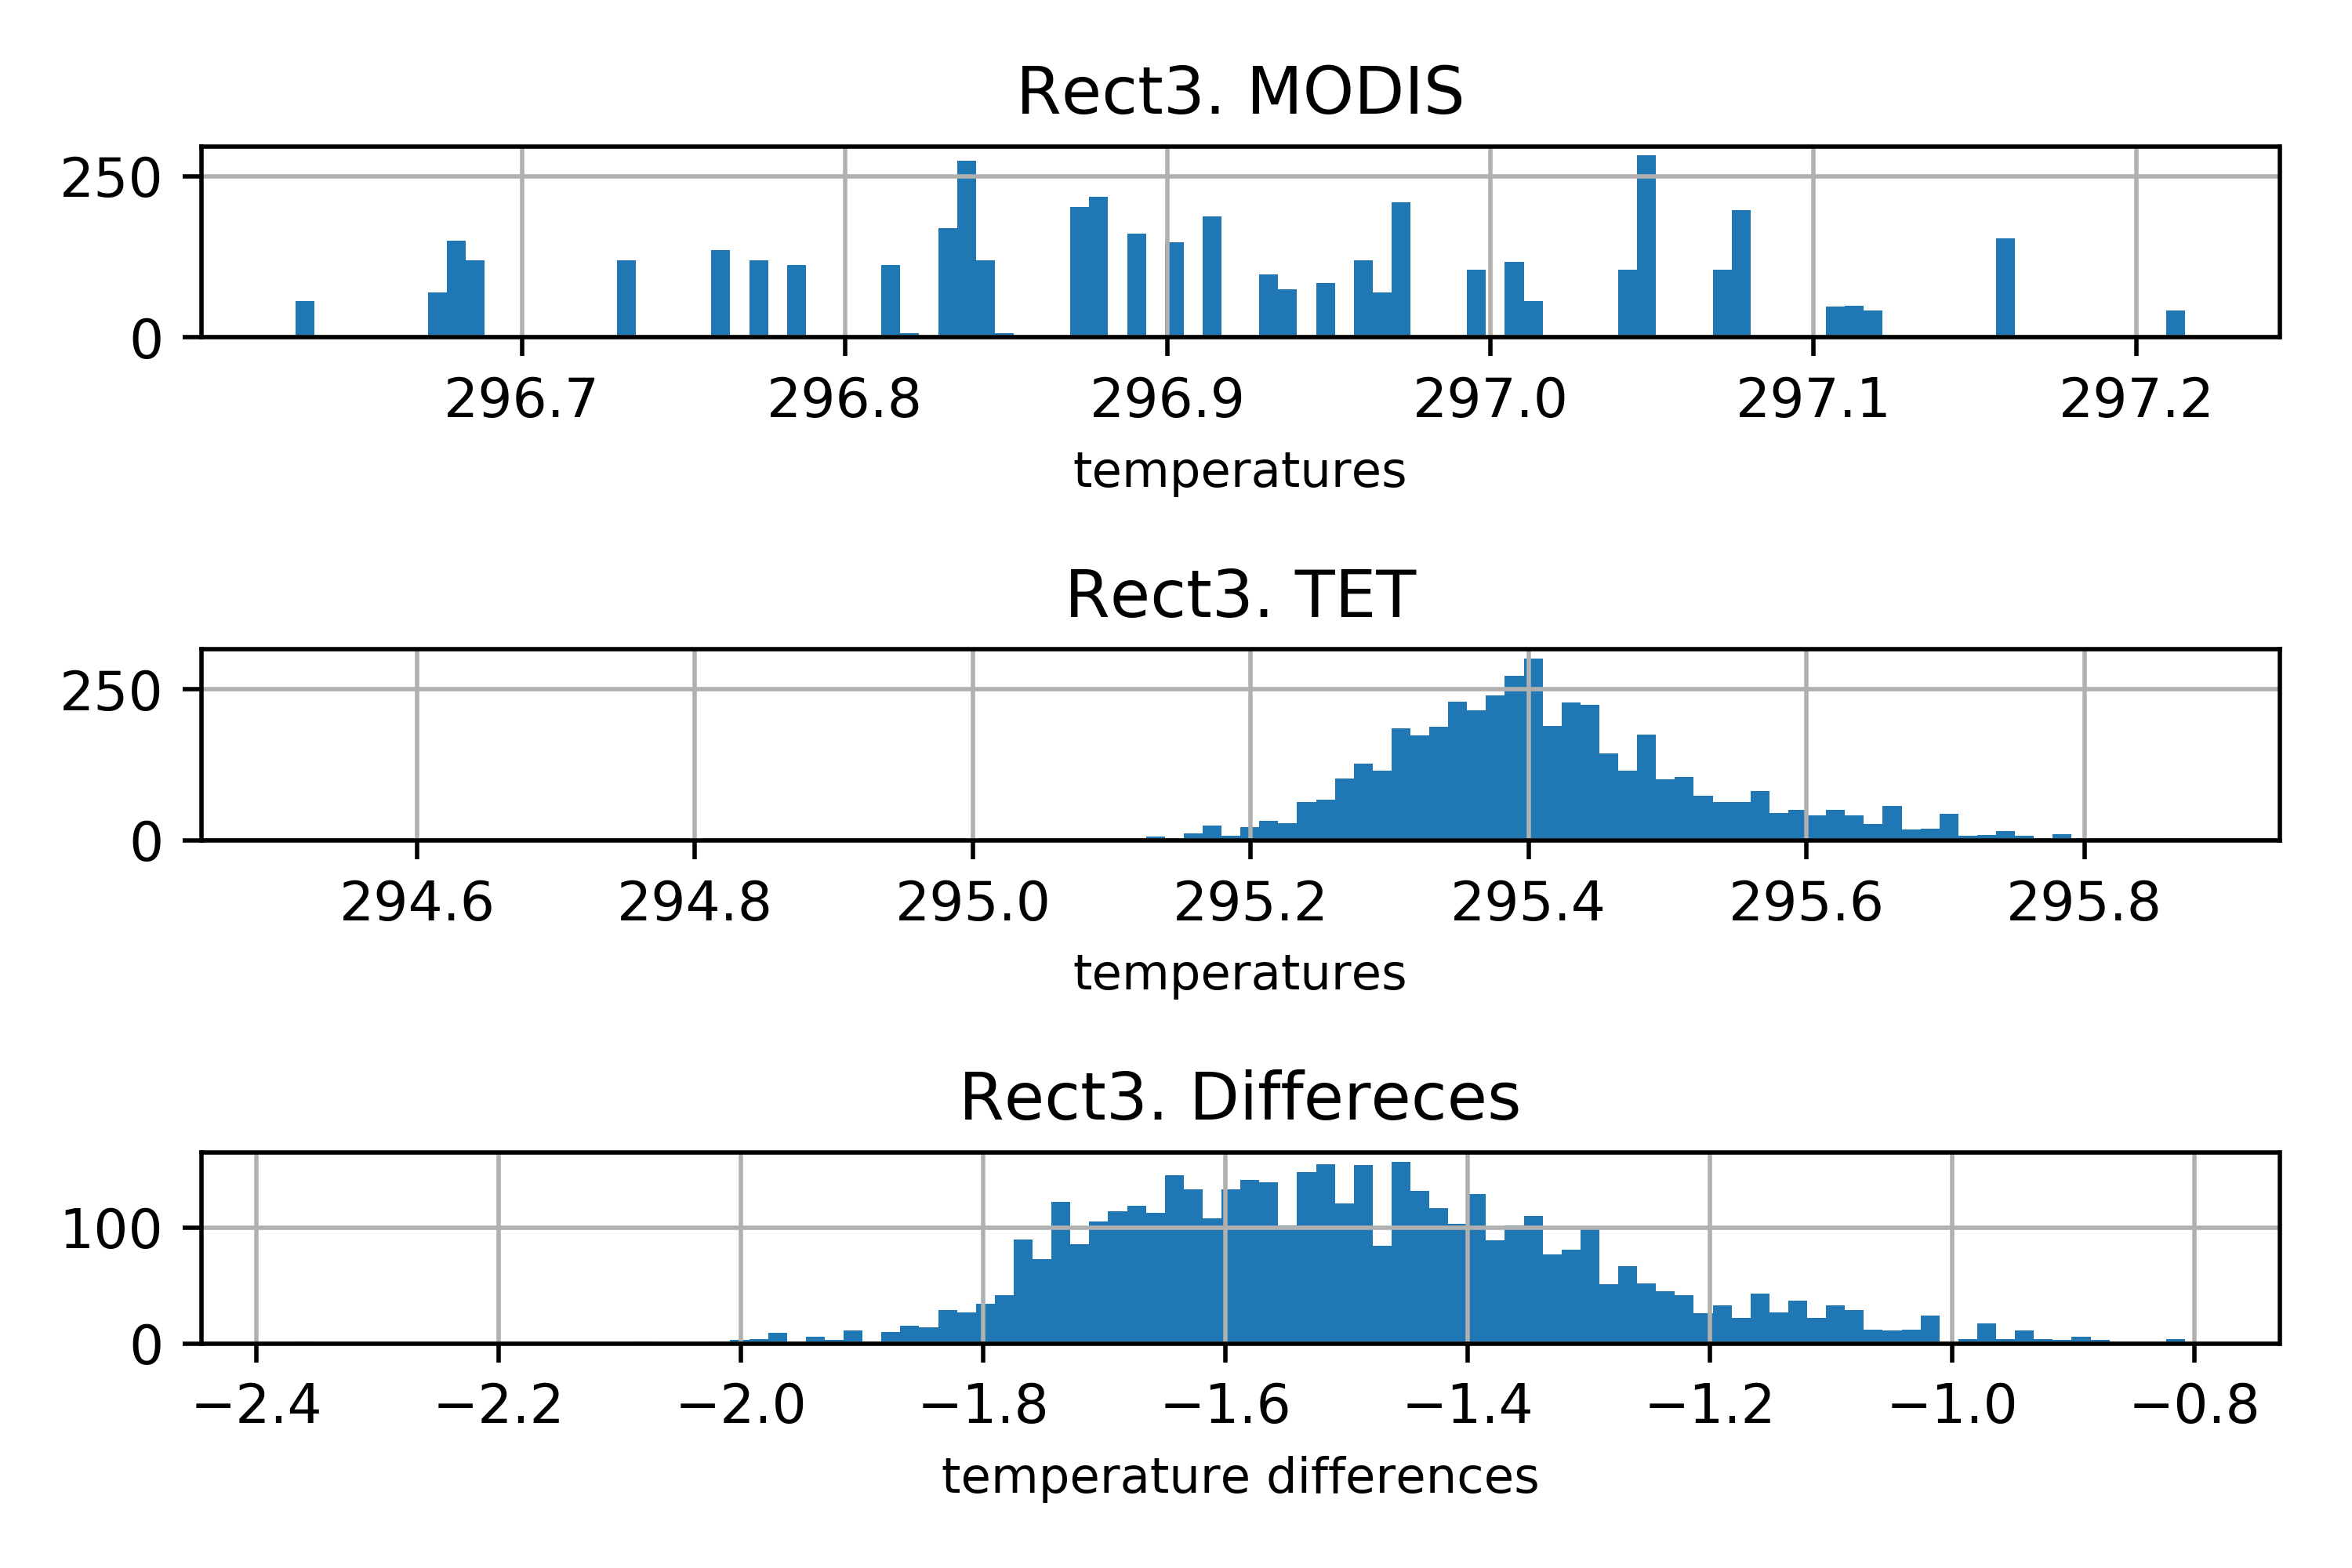
\includegraphics[width = 0.48\linewidth]{rect3_sc100.png}}
\vspace{0.1in}
\subfigure[Sub-area 3 with cale factor 1.10]{
\label{fig:hist_rect3_2}
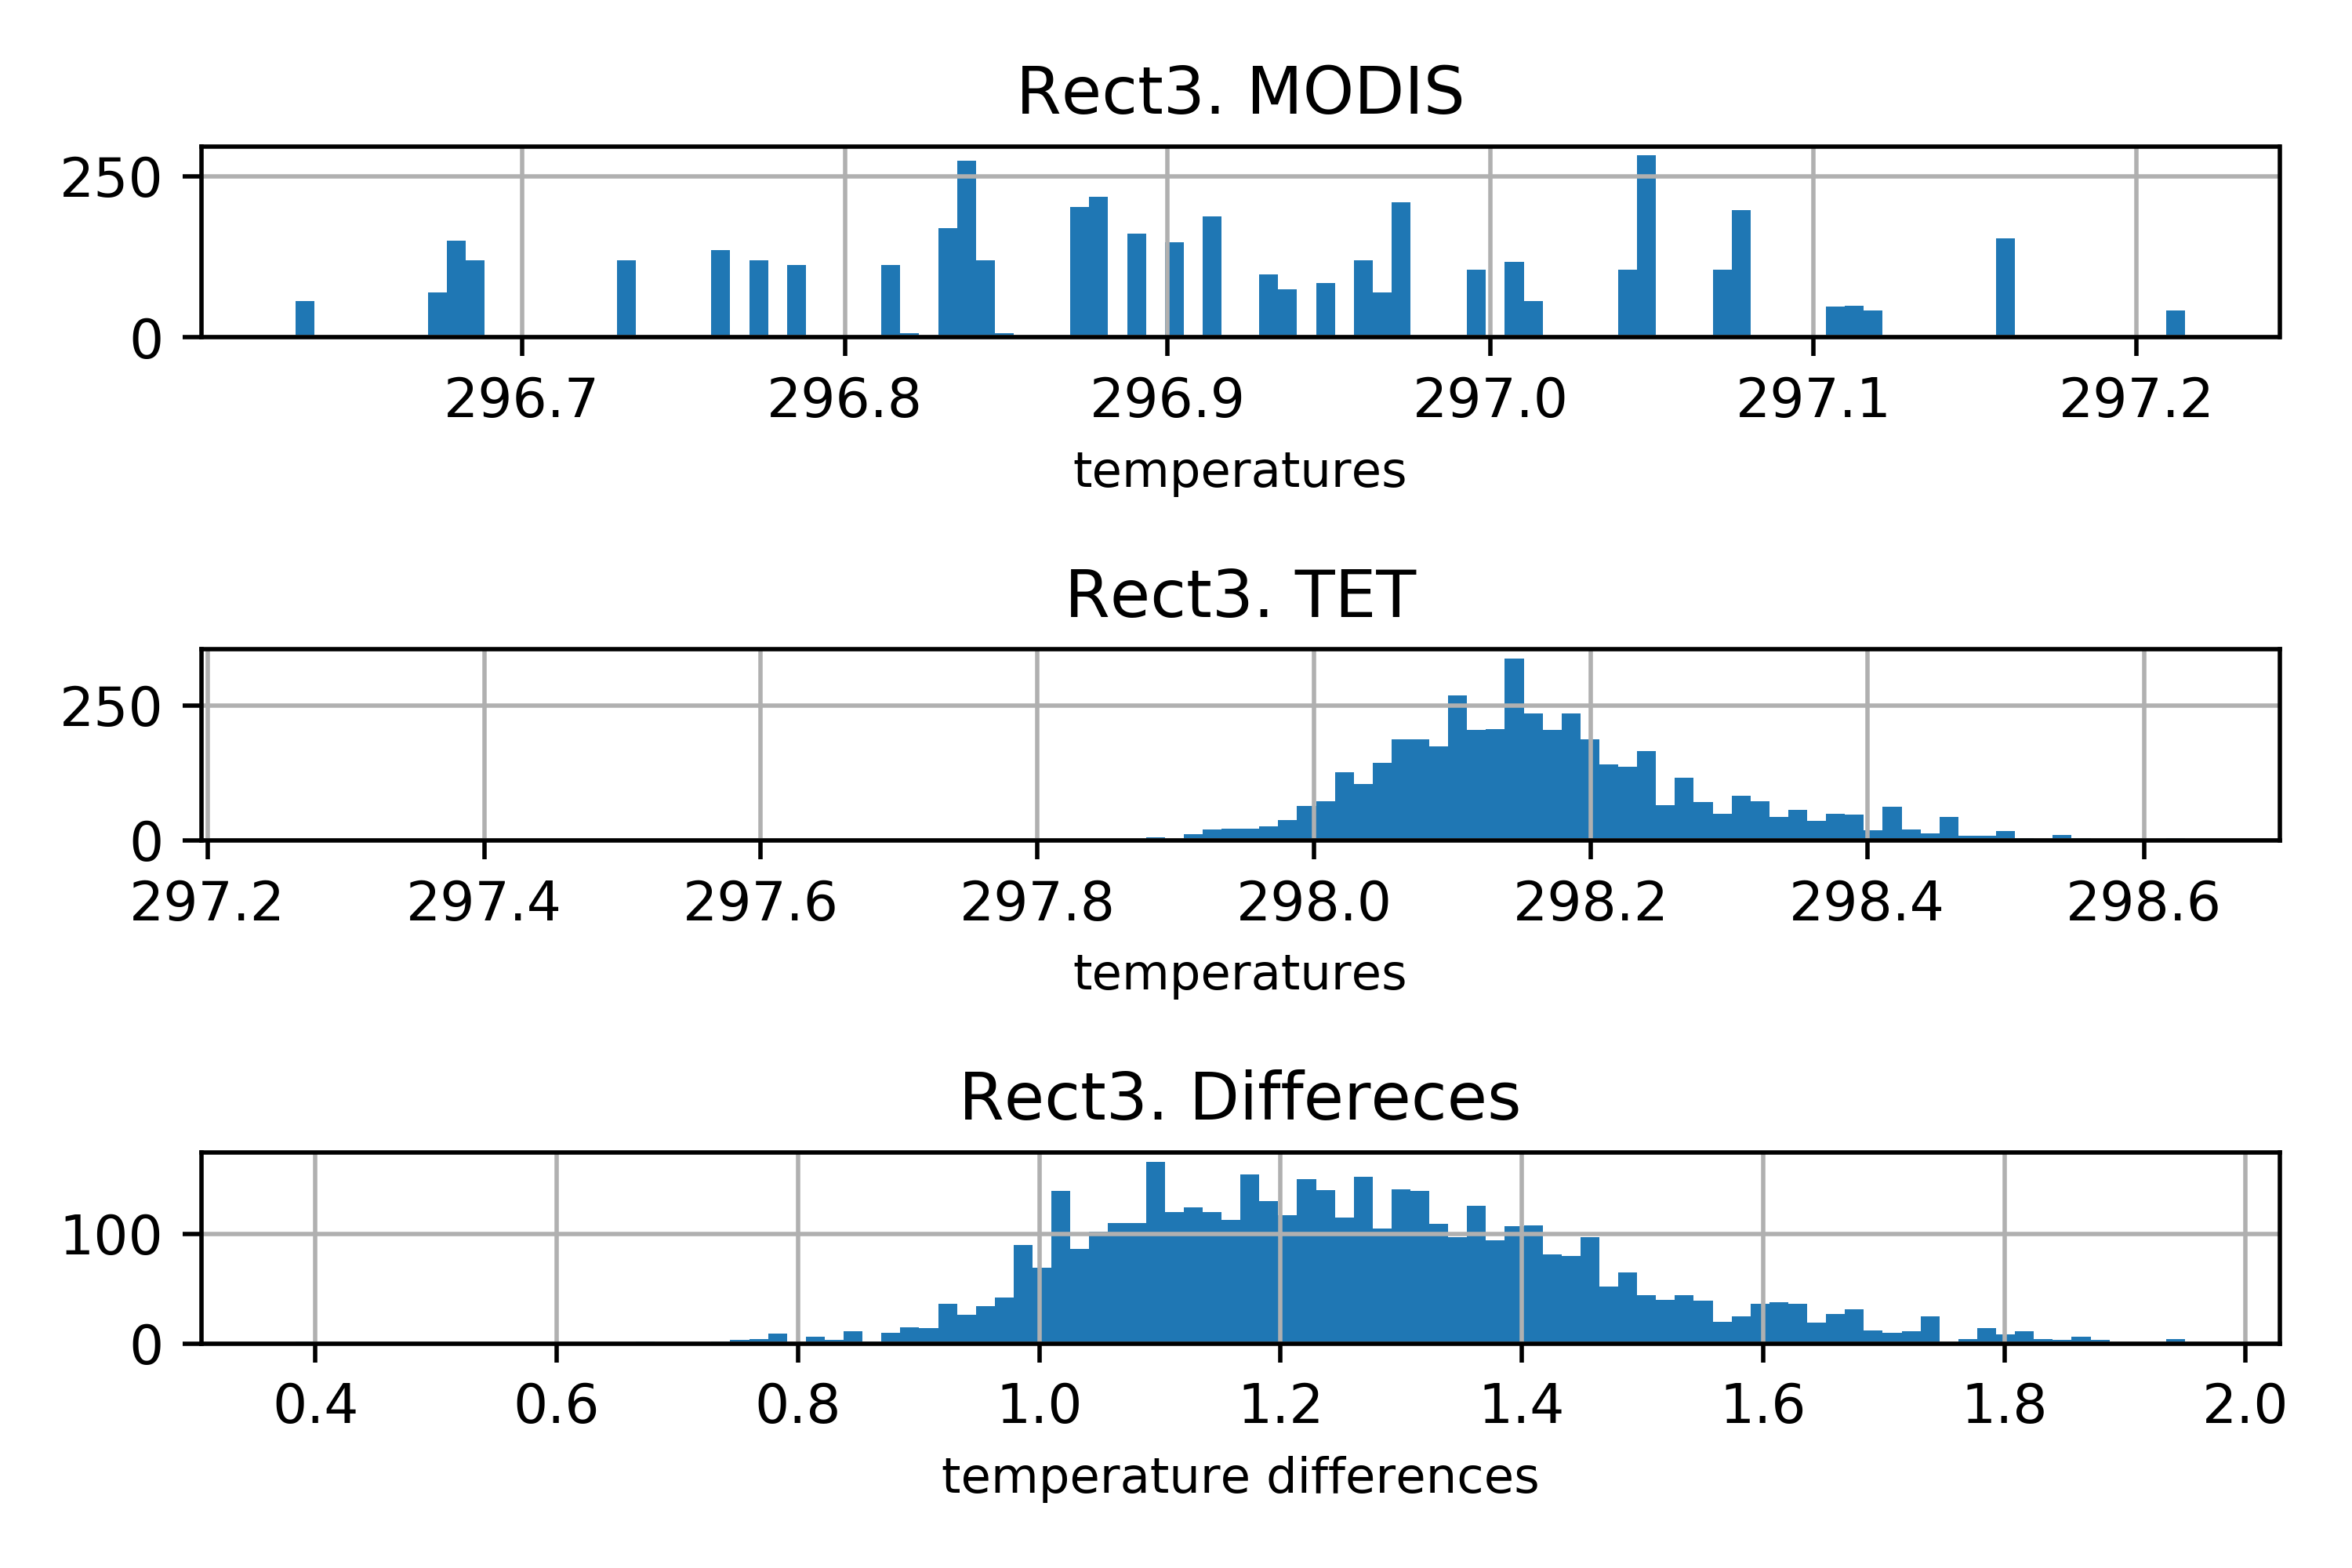
\includegraphics[width = 0.48\linewidth]{rect3_sc110.png}}

\hspace{0.5in}

\subfigure[Sub-area 4 with cale factor 1.00]{
\label{fig:hist_rect4_1}
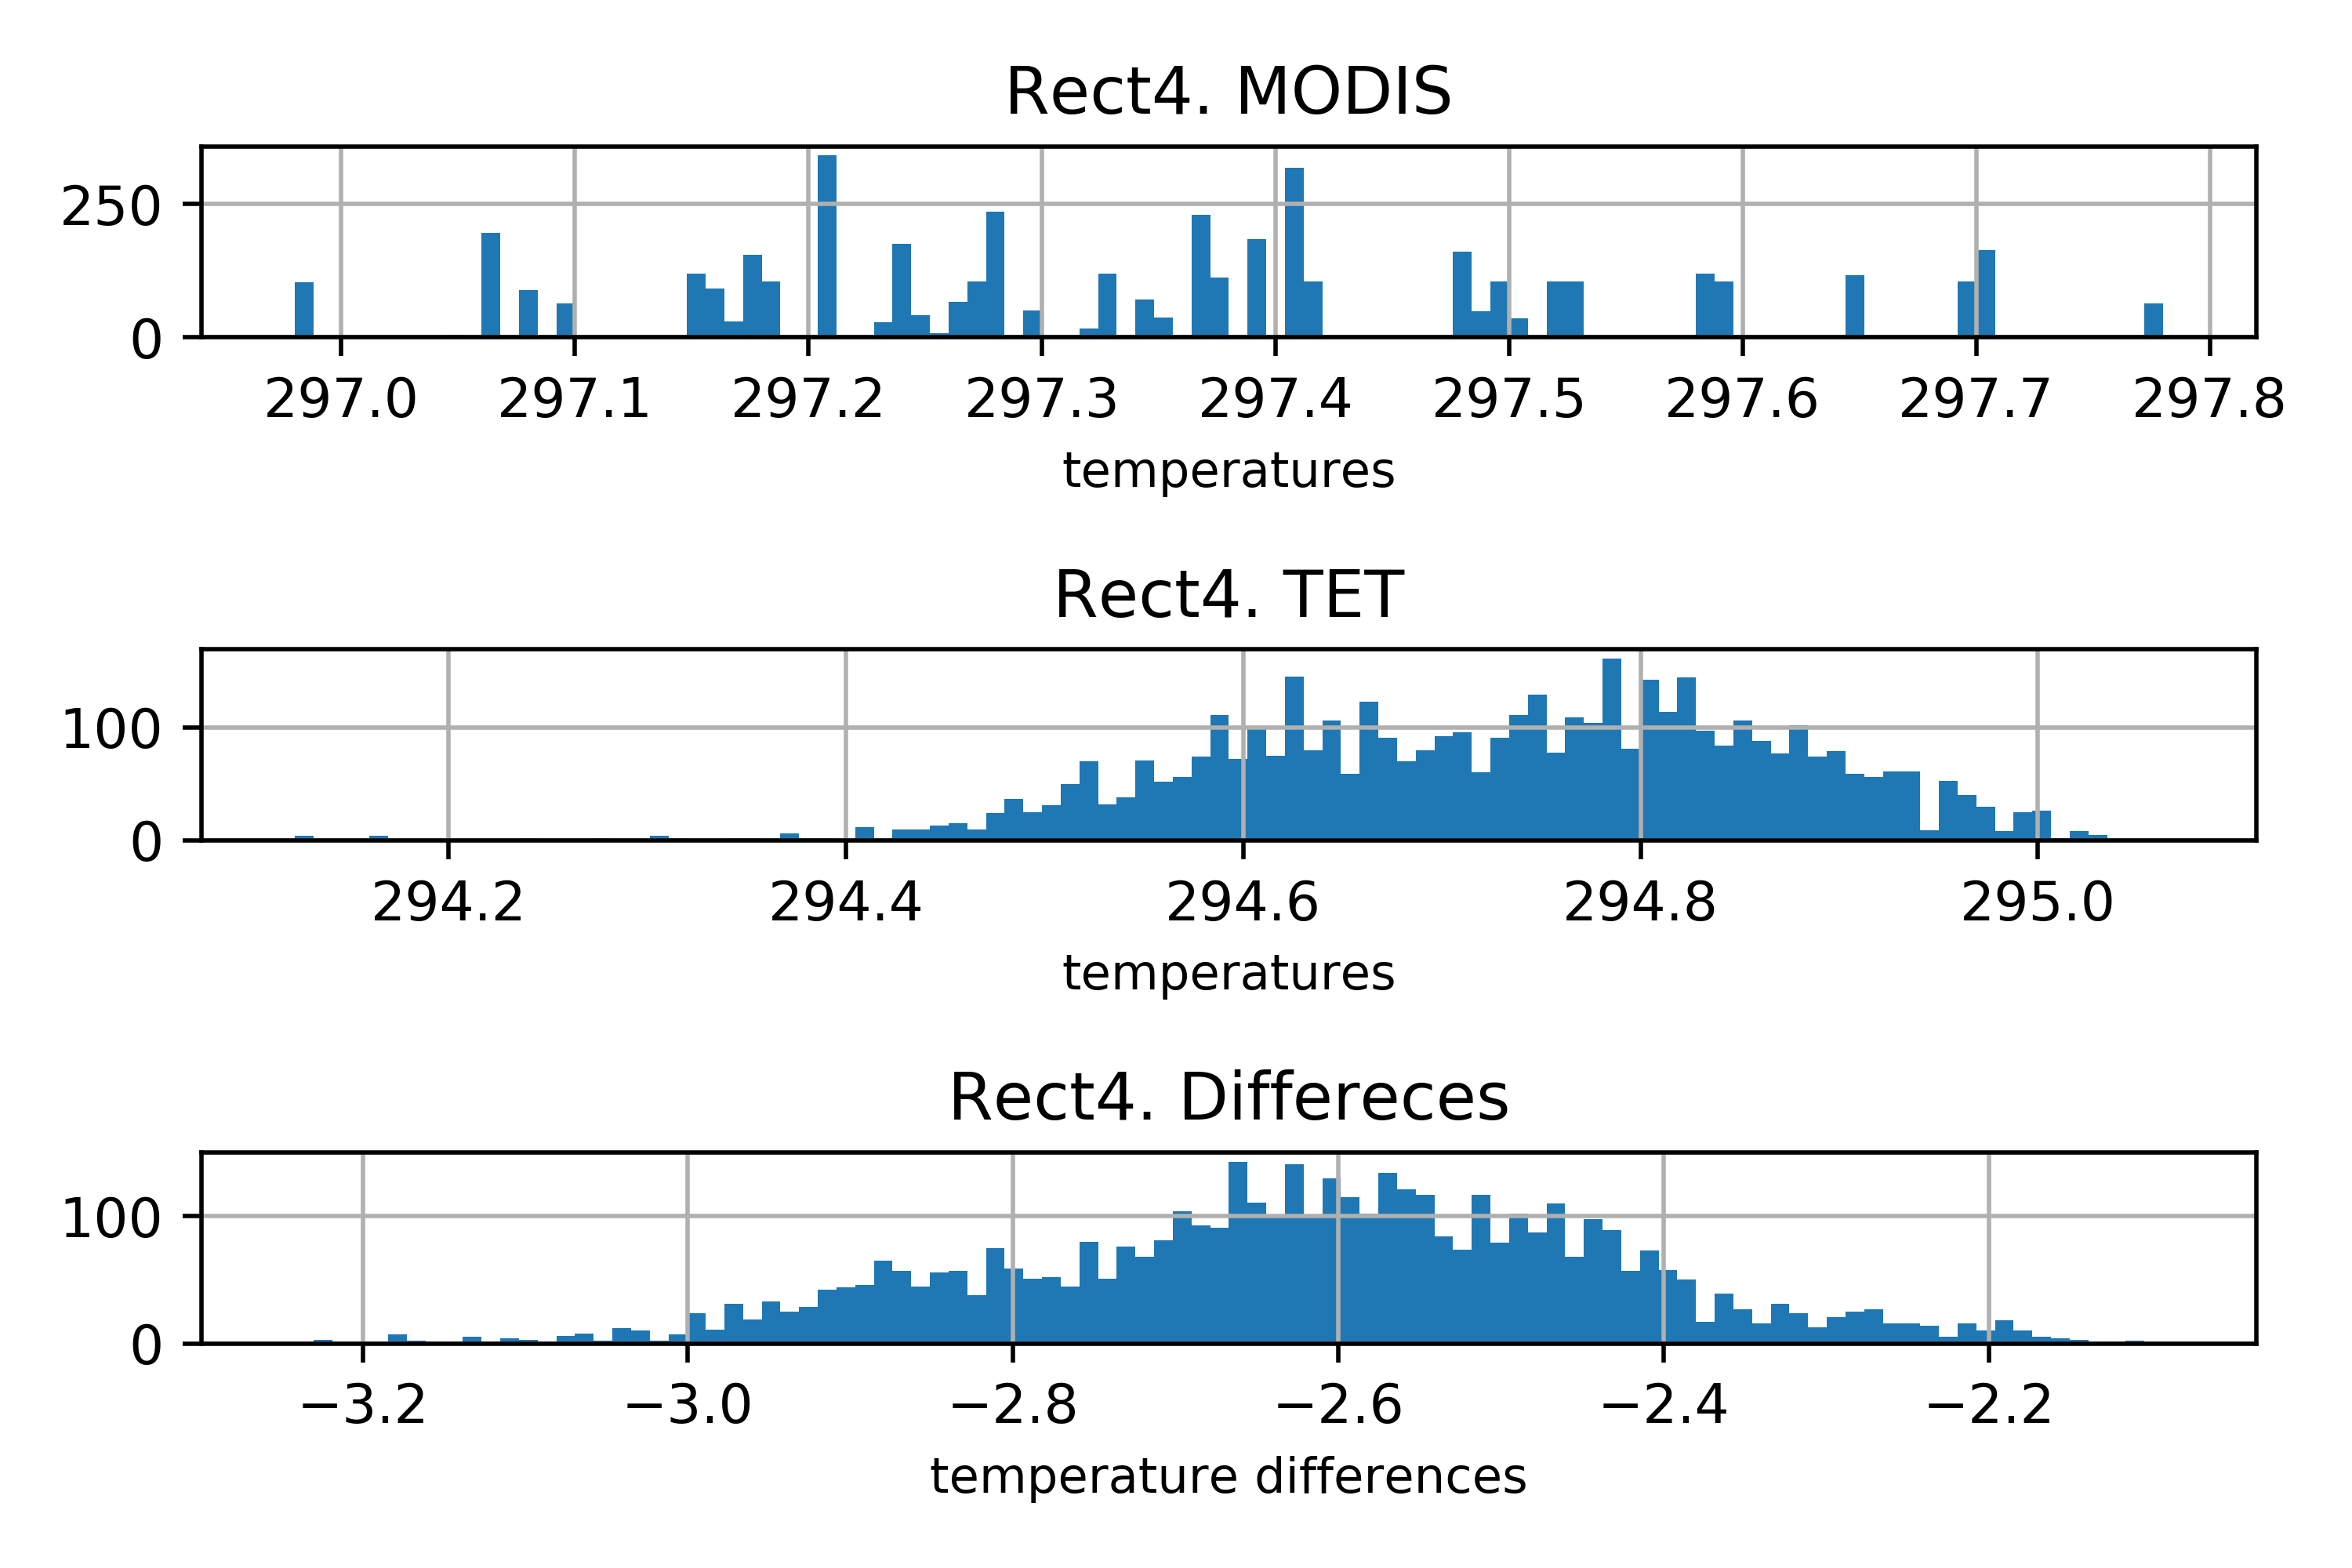
\includegraphics[width = 0.48\linewidth]{rect4_sc100.png}}
\vspace{0.1in}
\subfigure[Sub-area 4 with cale factor 1.10]{
\label{fig:hist_rect4_2}
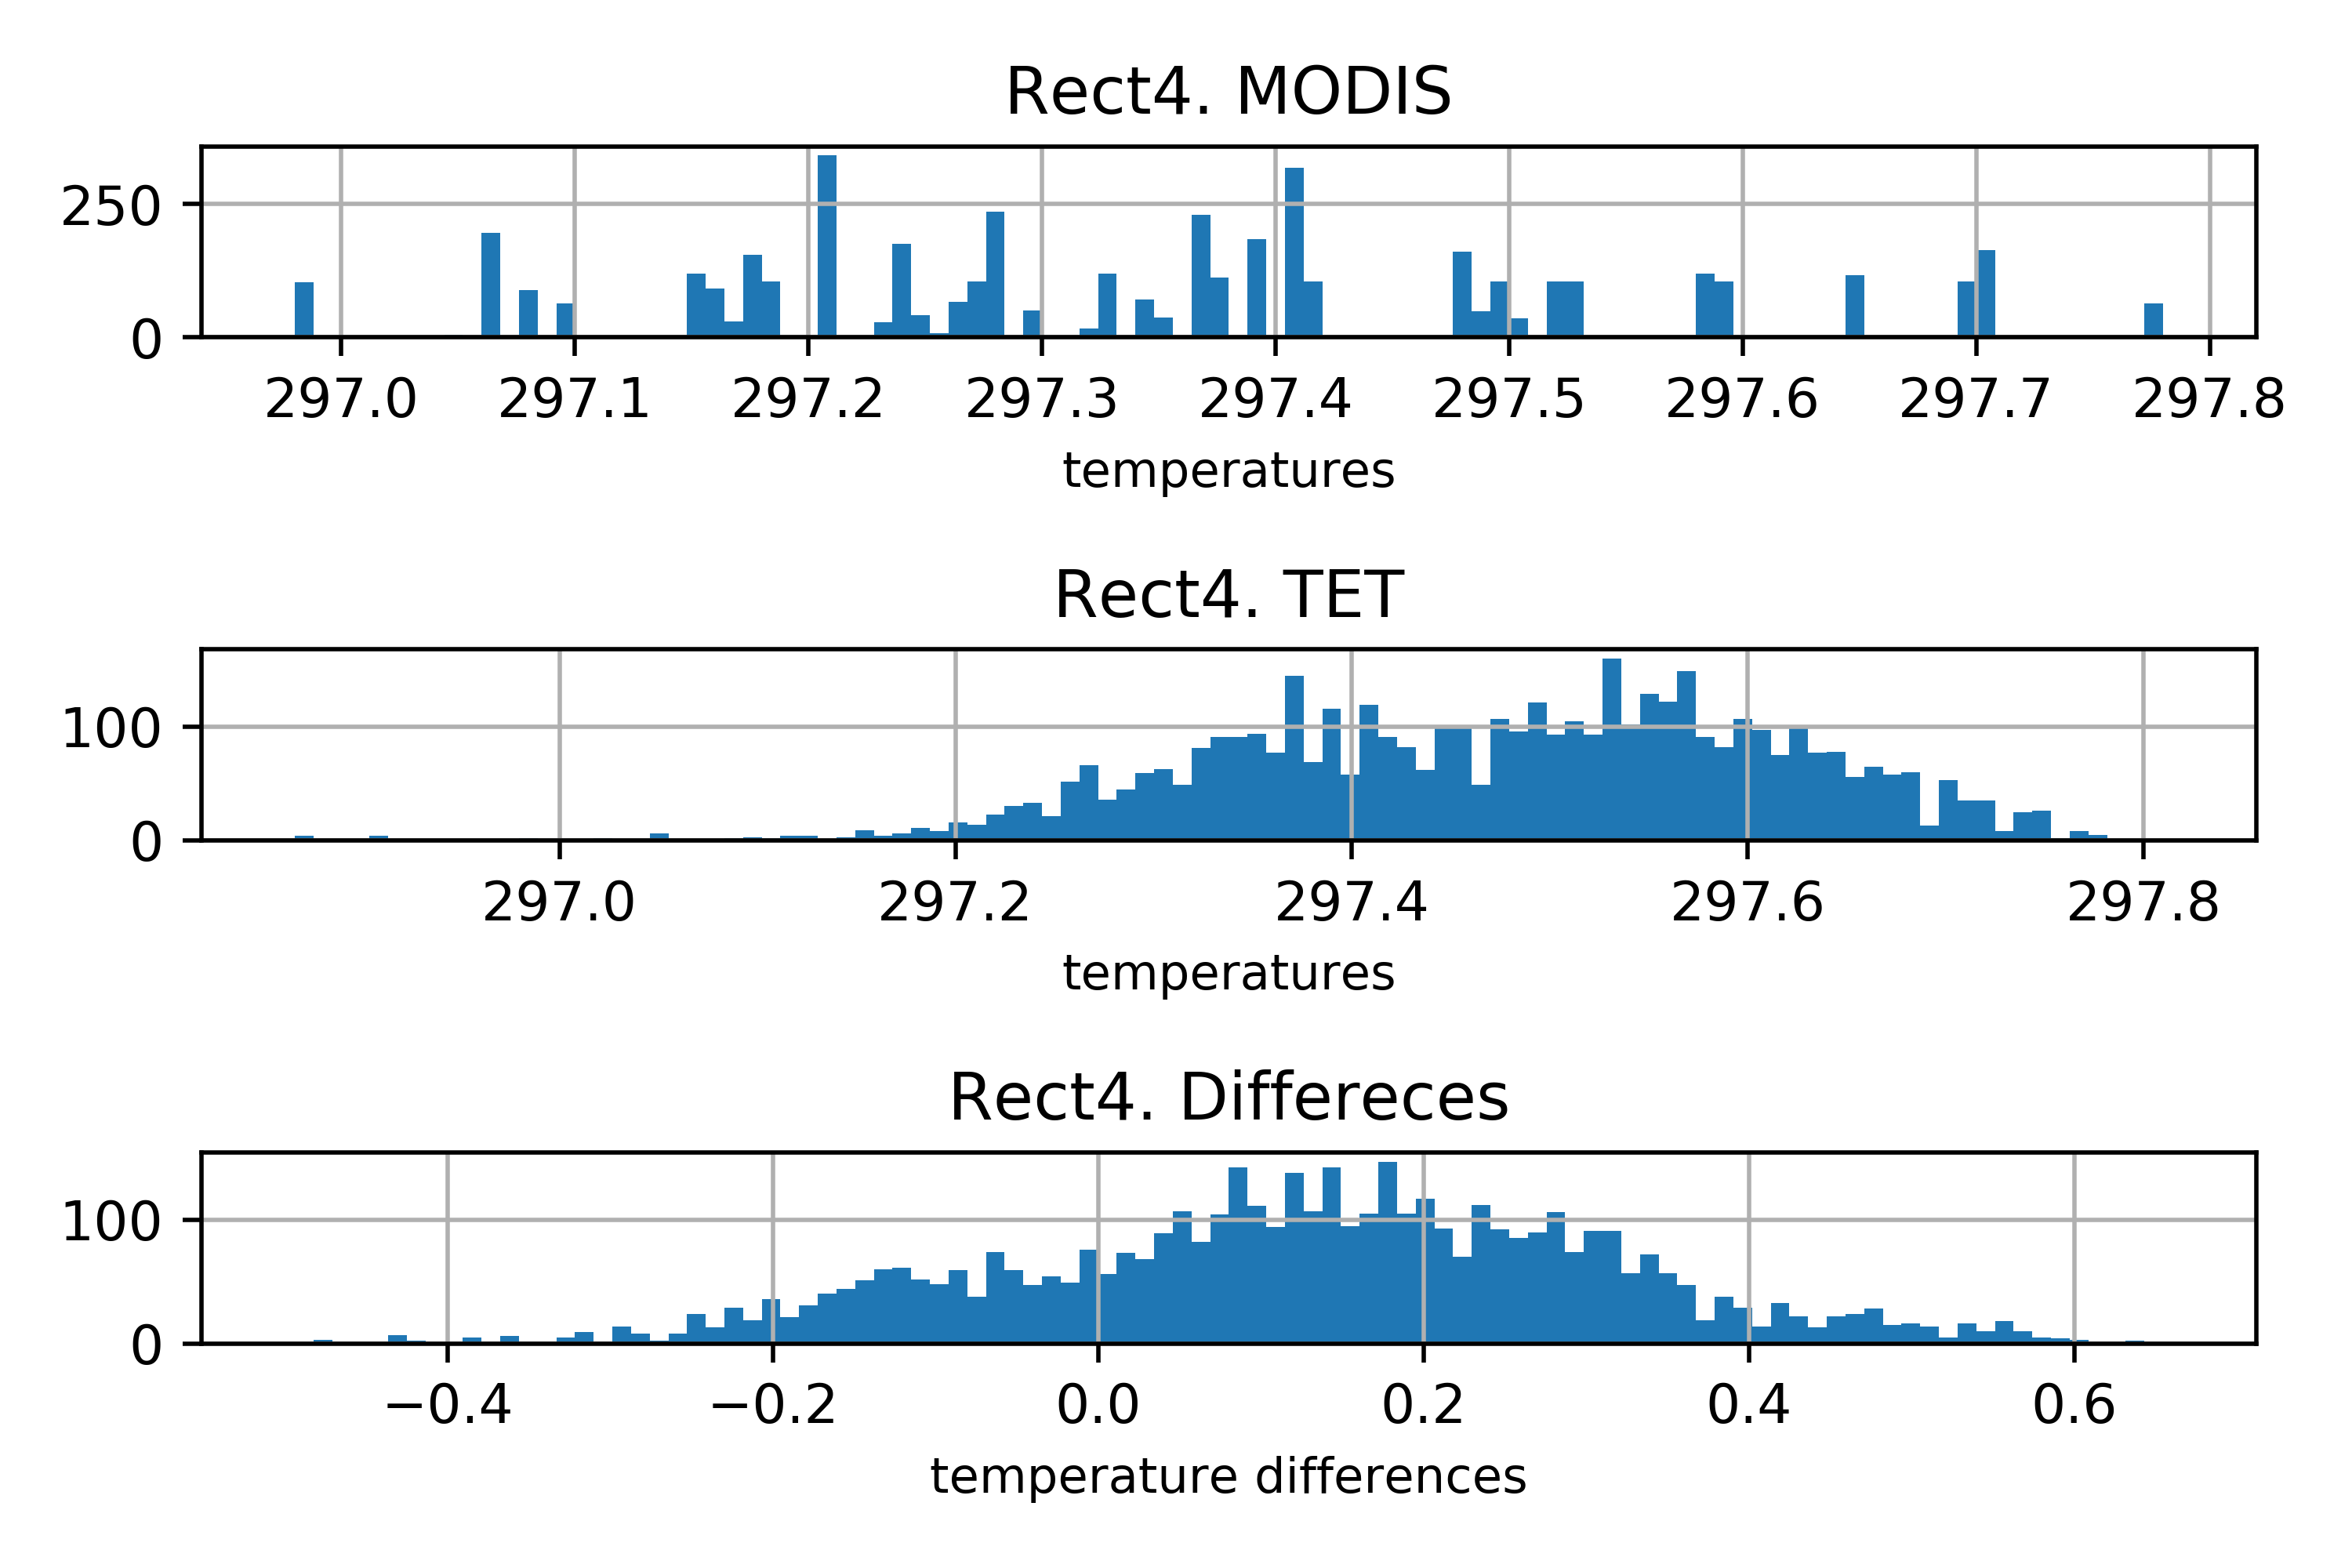
\includegraphics[width = 0.48\linewidth]{rect4_sc110.png}}

\caption{Histograms of MODIS SST, TET-1 MIR band imagry and their differences with different scale factor}
\label{fig:hist_rect_all}
\end{figure}

\noindent In Figure \ref{fig:hist_rect_all}, it is clear that the histograms of the same sub-area of MODIS SST are the same. For the TET-1 MIR band temperature maps with differnet scale factors, the shapes of the histograms of the same sub-area, which are the second row of each sub-figures, are almost identical. But looking carefully we will notice that for the histograms of TET-1 MIR band temperature map with different scale factors, the x-axes are shifted to the left, which means the pixel values of all pixels inside one sub-area are increased with a certain value. The same for the temperature differences between MODIS SST and the TET-1 MIR band temperature map. To make it more clear, two sub-areas are selected and their histograms with all the five scale factors are shown in Figure \ref{fig:rect1_sc_all} and Figure \ref{fig:rect4_sc_all}.\\

\begin{figure}[!htbp]
\centering
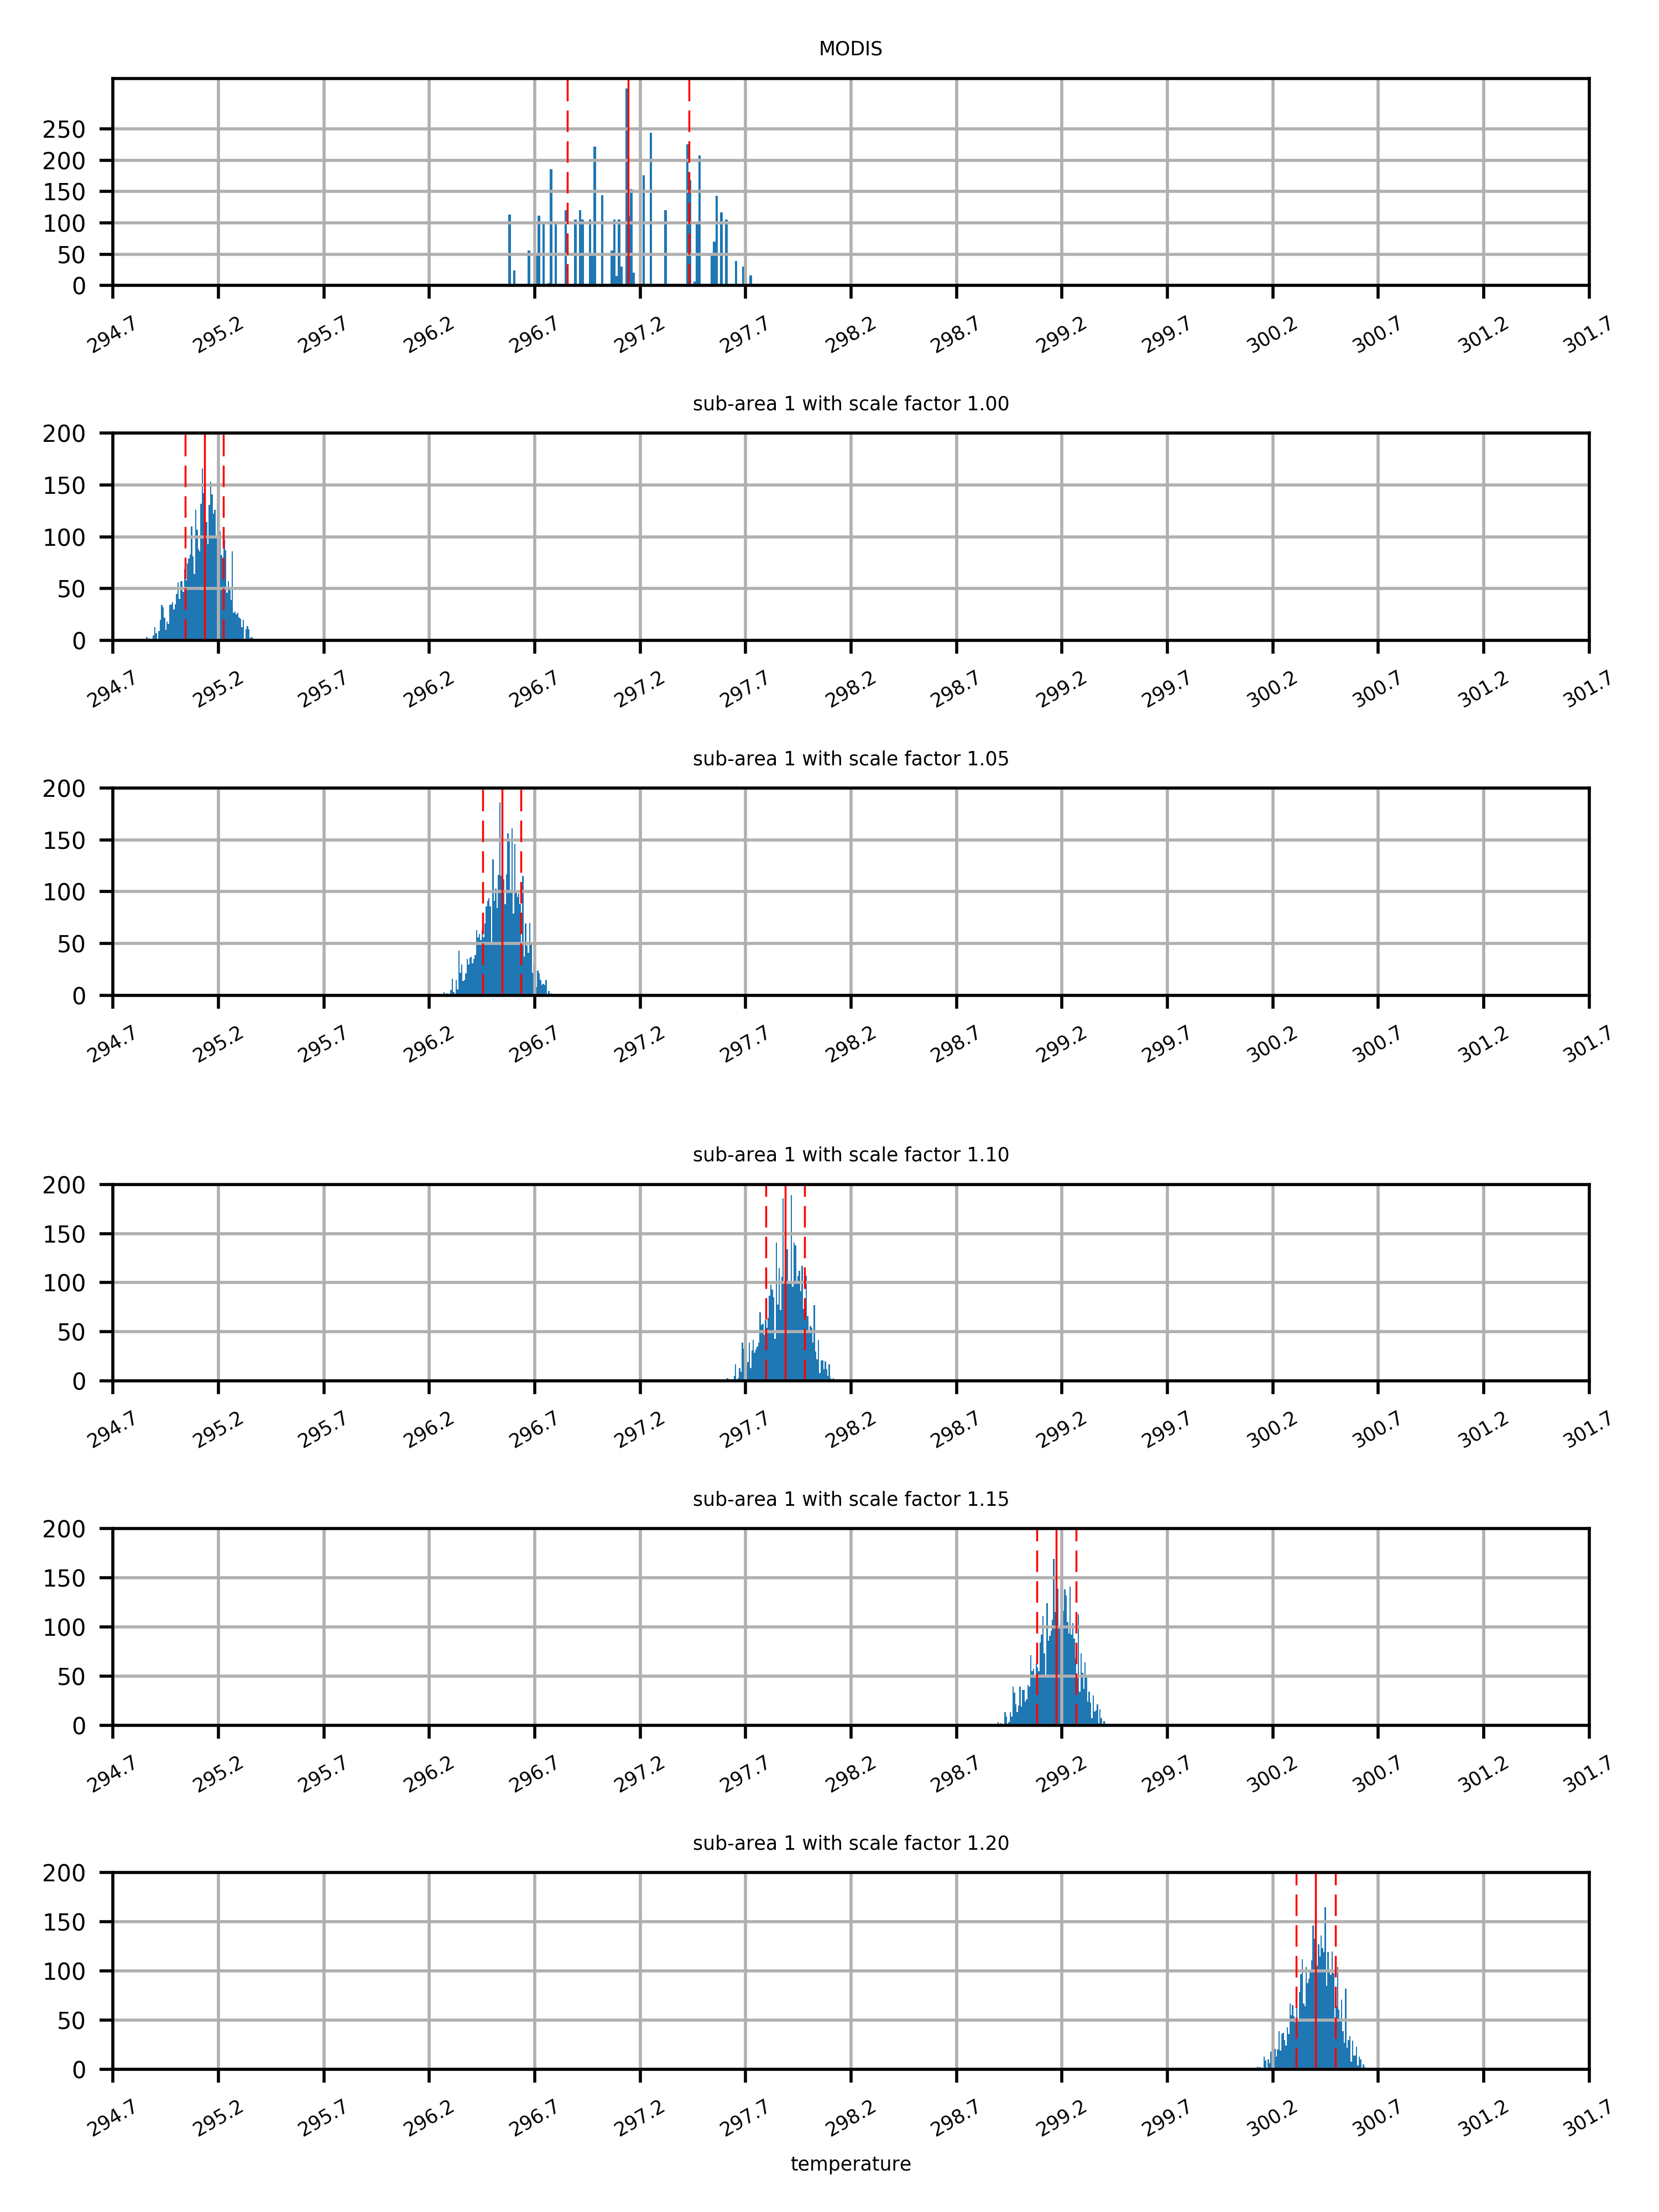
\includegraphics[width = 1.0\textwidth]{rect1_sc_all.png}
\caption{Histograms of MODIS SST and TET-1 MIR band imageries with all the five scale factors in sub-area 1. The red solid line in each histogram denotes the mean value and the red dashed line the standard deviation.}
\label{fig:rect1_sc_all}
\end{figure}

\begin{figure}[!htbp]
\centering
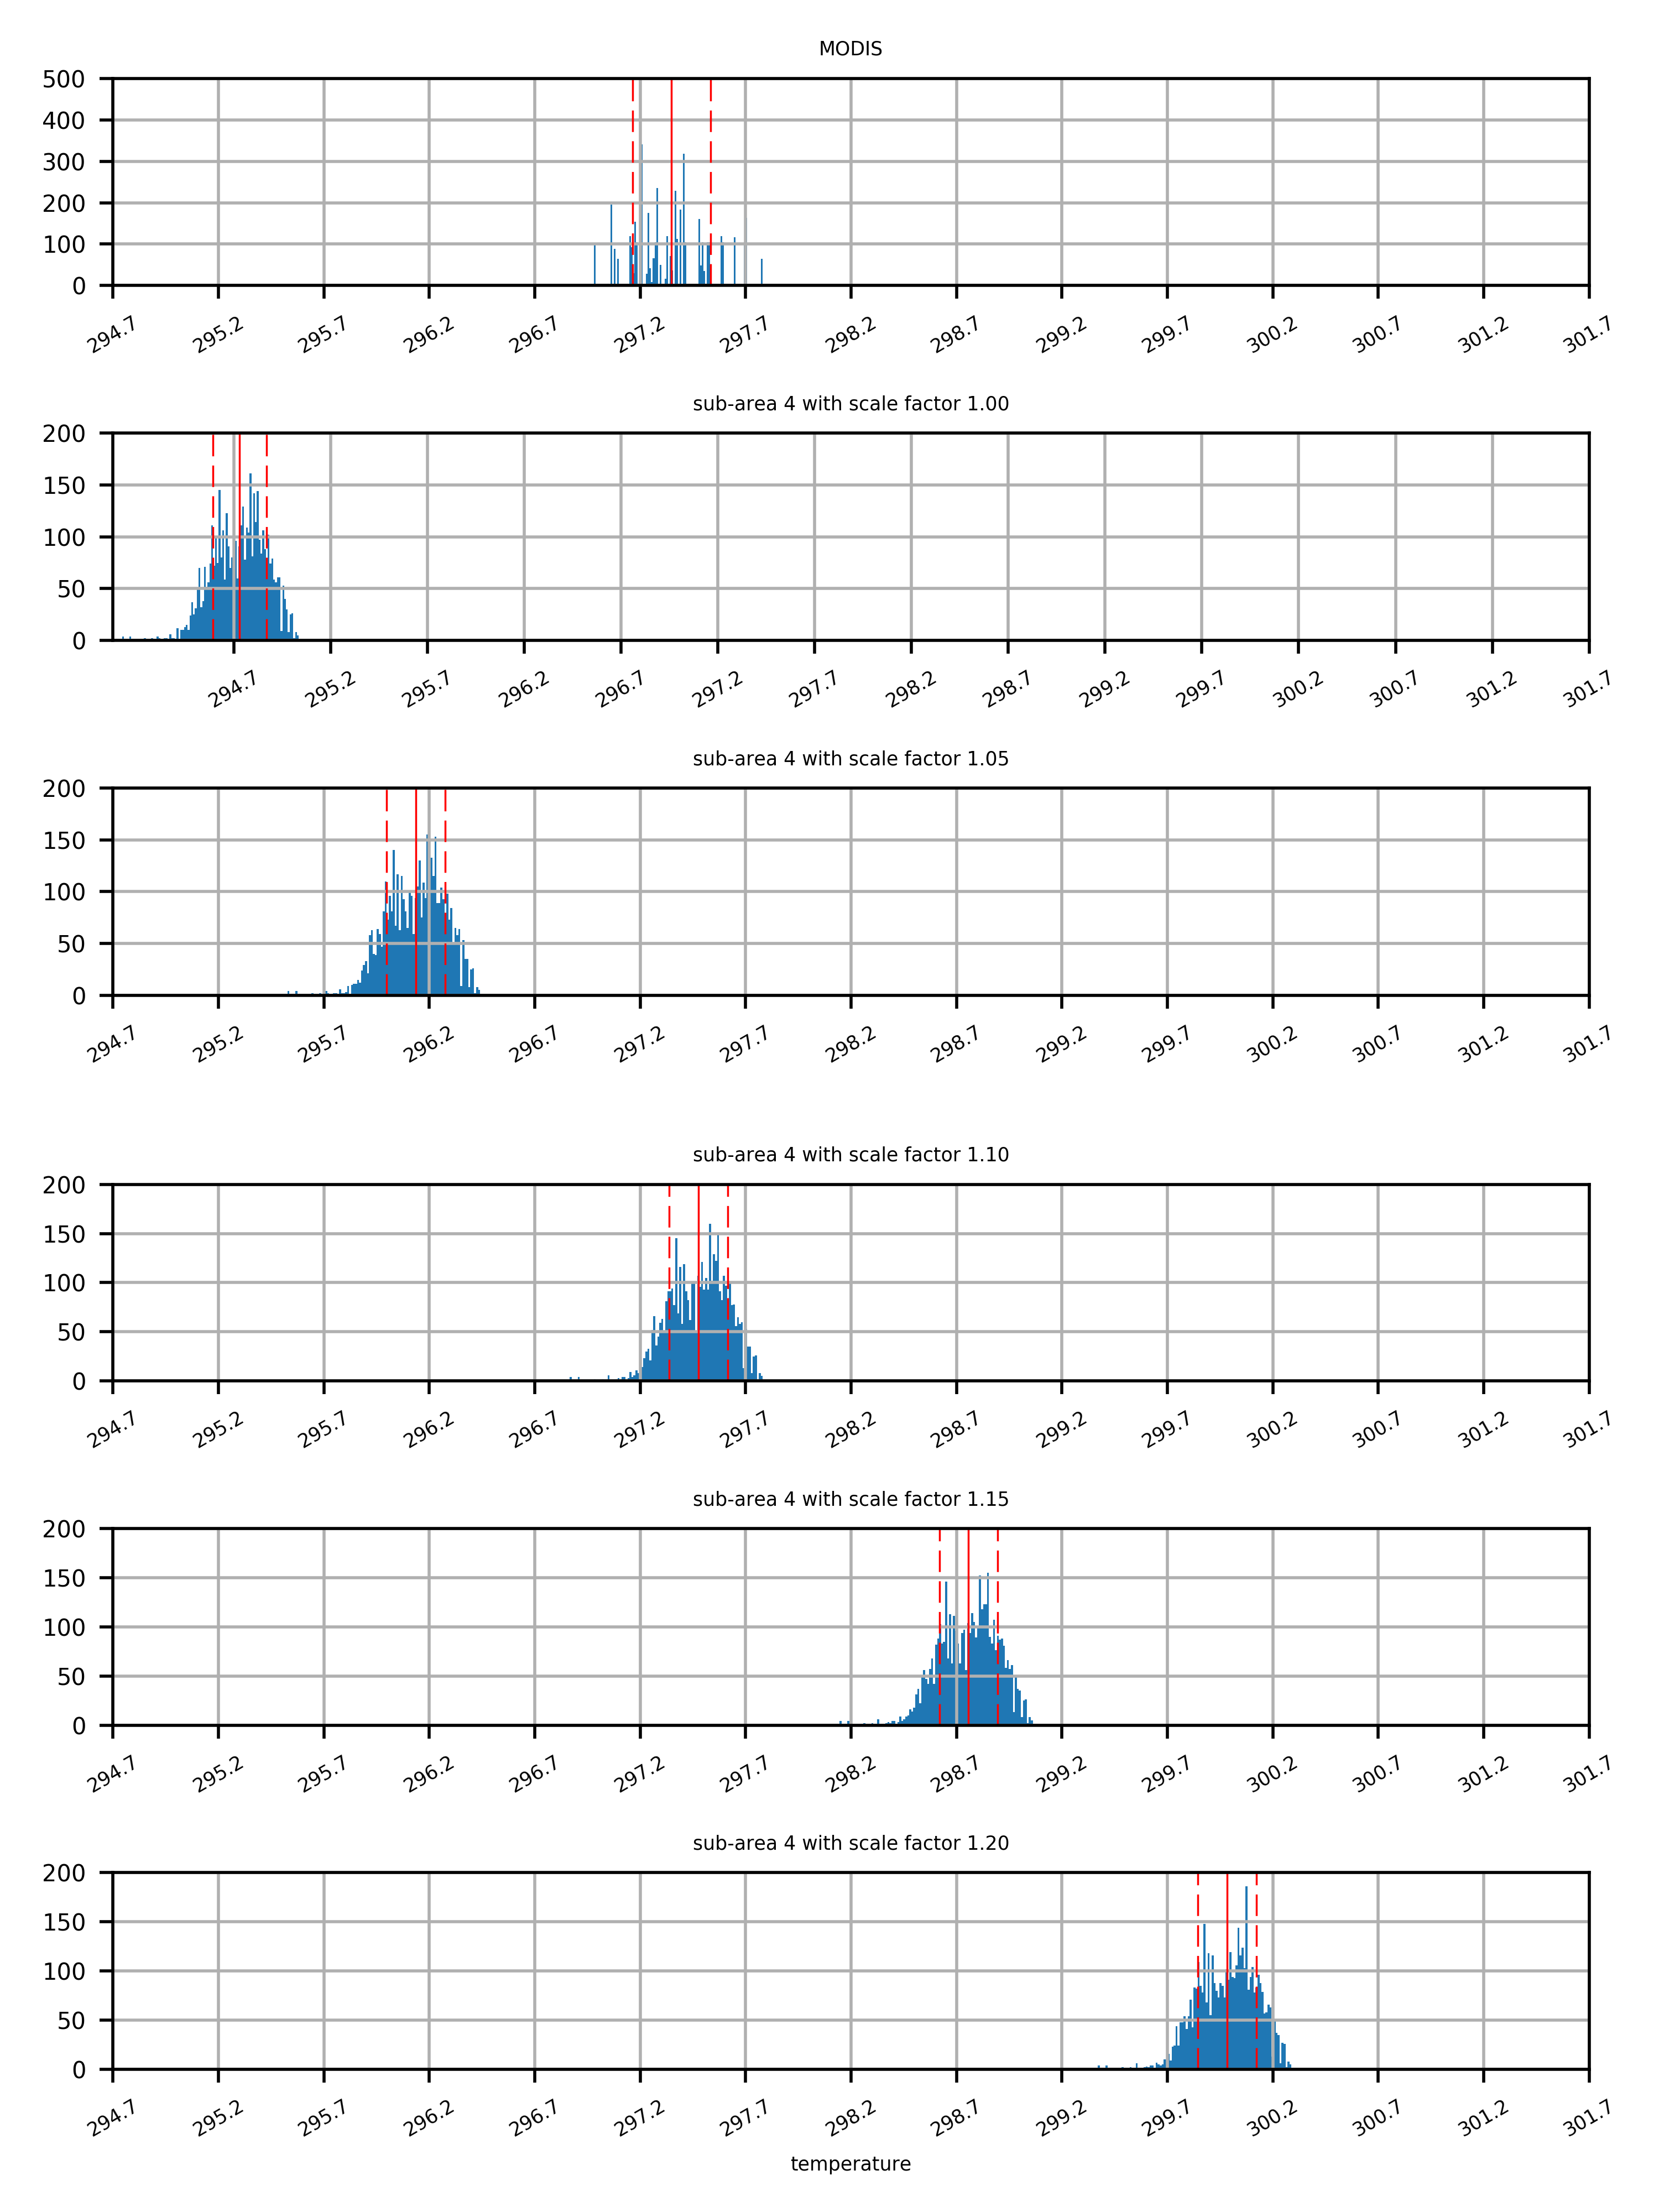
\includegraphics[width = 1.0\textwidth]{rect4_sc_all.png}
\caption{Histograms of MODIS SST and TET-1 MIR band imageries with all the five scale factors in sub-area 4. The red solid line in each histogram denotes the mean value and the red dashed line the standard deviation.}
\label{fig:rect4_sc_all}
\end{figure}

\noindent Figure \ref{fig:rect1_sc_all} and Figure \ref{fig:rect4_sc_all} obviously show that with the increment the scale factor, the histograms of the sub-areas will be shifted to the right while the shapes are almost unchanged. The mean temperature of each histogram acts as a linear function of scale factor while the standard deviations are very stable, which means the shapes of the histograms are keeping unchanged. Consequently, the mean temperature of all pixels within one sub-area can be used as representative for this sub-area and show how temperatures vary with the change of scale factor.\\

\noindent But we do not use only the mean temperature of one sub-area. As stated in Section 4.1.1, the mean temperature over all the sub-areas will be calculated to compare with the same value of MODIS SST. The histograms of pixels located inside all the sub-areas are given in Figure \ref{fig:hist_all_rect} and Figure \ref{fig:rect_all_sc_all}. For MODIS SST, due to the reasons of upsampling, noisy and missing value etc, its histograms of the sub-areas are sparse and concentrate in fewer values. Its shape is a bit skewed left but its main part is symmetric. Furthermore, the main part of the histogram of all sub-areas of MODIS SST shares the similar shape with the histograms of all sub-areas of TET-1 MIR band surface temperature map. For TET-1 MIR band surface temperature map, the behavior of histograms of all sub-areas is the same as the histograms of individual sub-area as stated before. Hence it is reasonable and reliable to use the mean temperature over all the sub-areas in both MODIS SST and TET-1 surface temperature product to do the comparison instead of using the histogram all the time.\\

\begin{figure}[!htbp]
\centering
\subfigure[Scale factor 1.00]{
\label{fig:hist_rect_all_1}
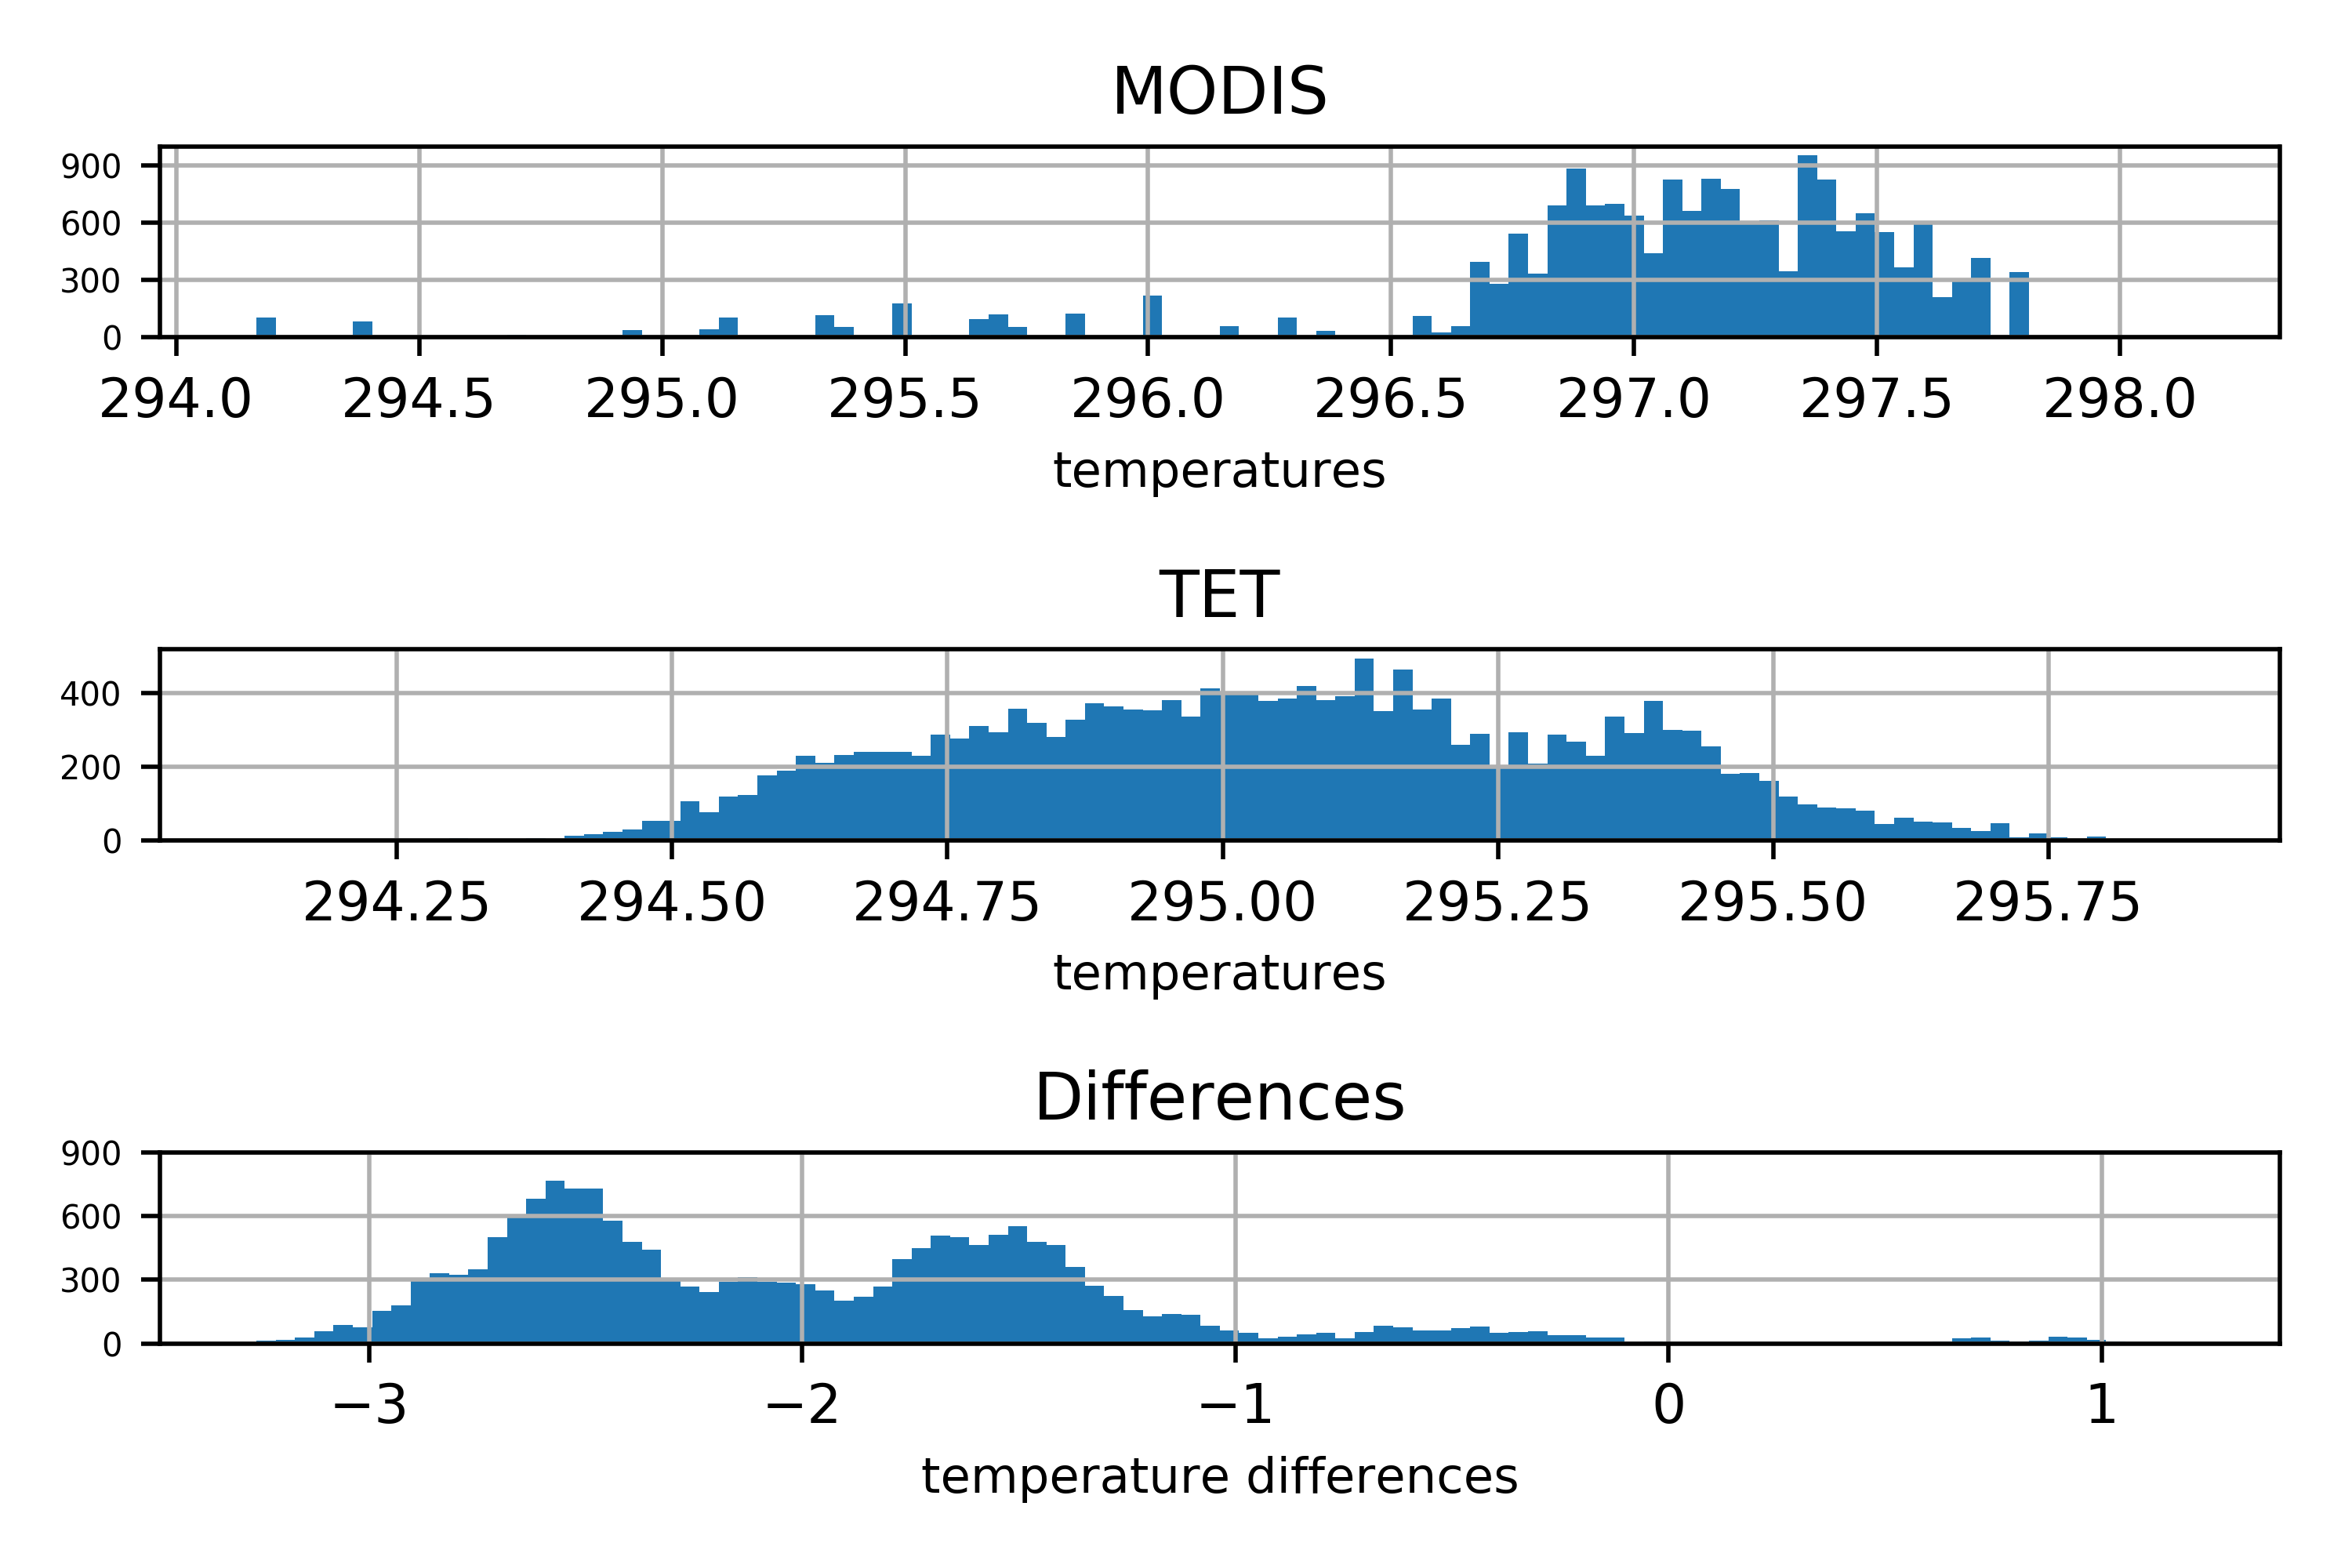
\includegraphics[width = 0.48\linewidth]{rect_all_sc100.png}}
\vspace{0.1in}
\subfigure[Scale factor 1.10]{
\label{fig:hist_rect_all_2}
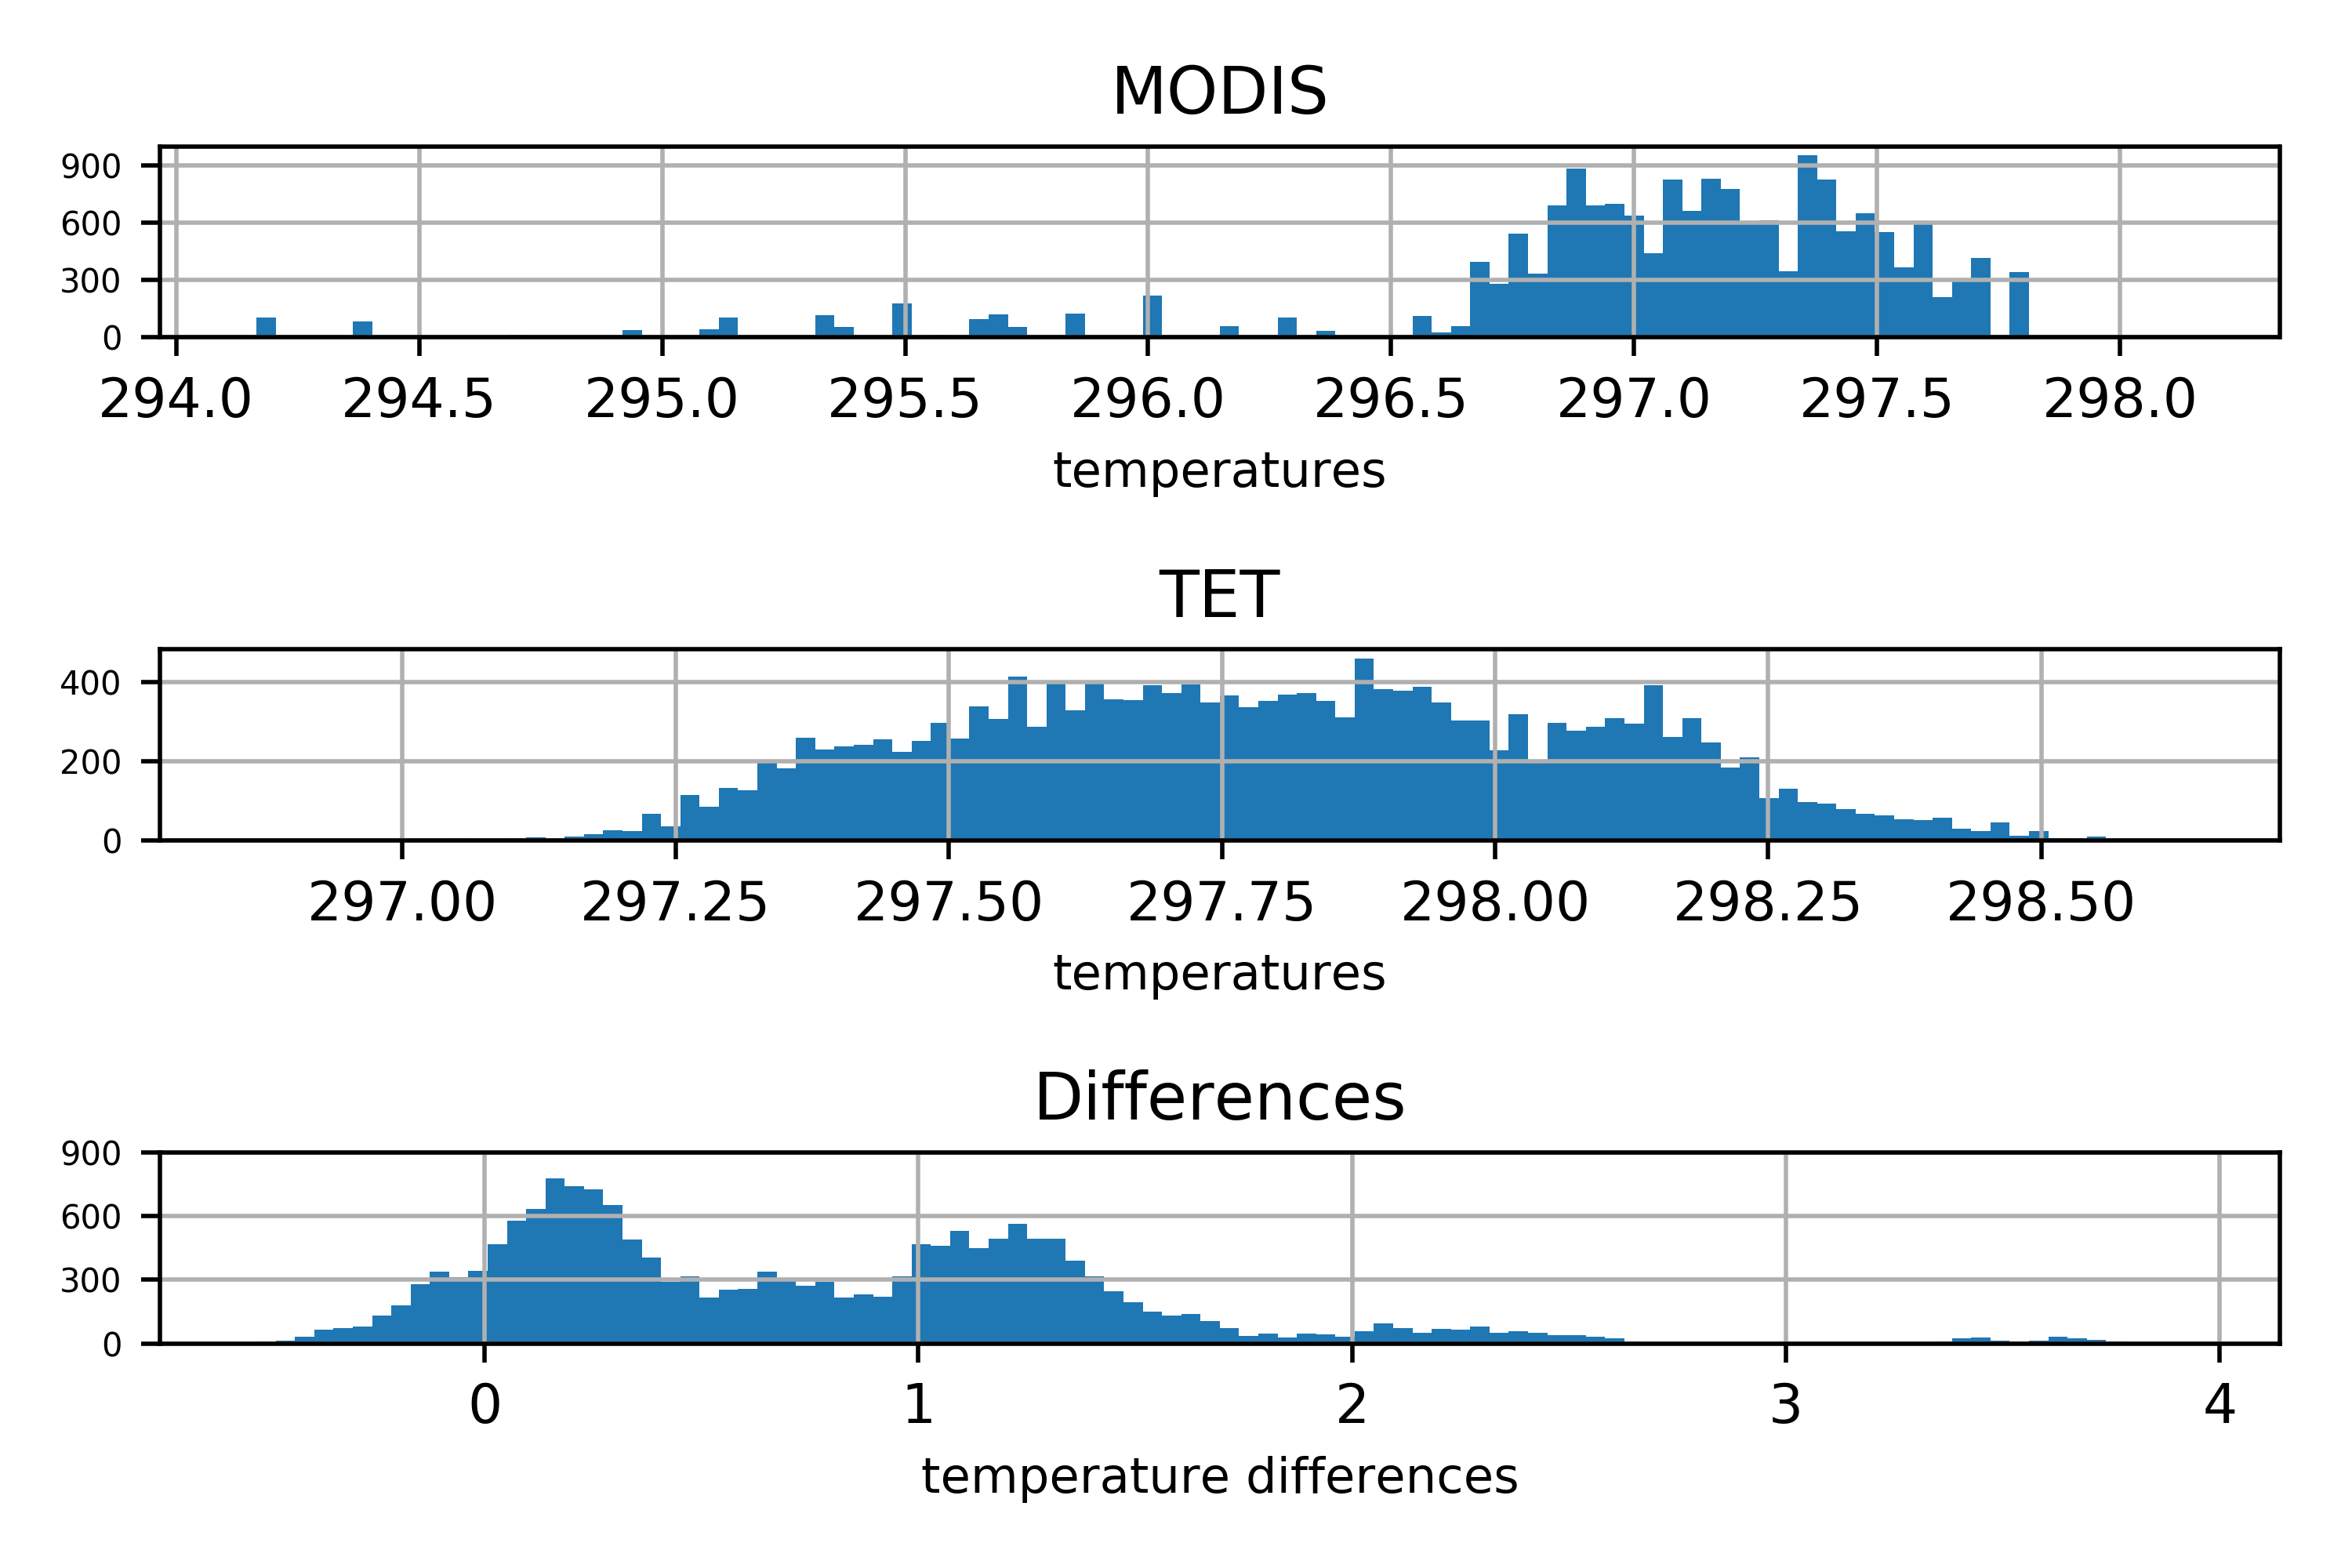
\includegraphics[width = 0.48\linewidth]{rect_all_sc110.png}}
\caption{Histograms of all sub-areas of MODIS SST, TET-1 MIR band imagry and their differences with different scale factor}
\label{fig:hist_all_rect}
\end{figure}

\begin{figure}[!htbp]
\centering
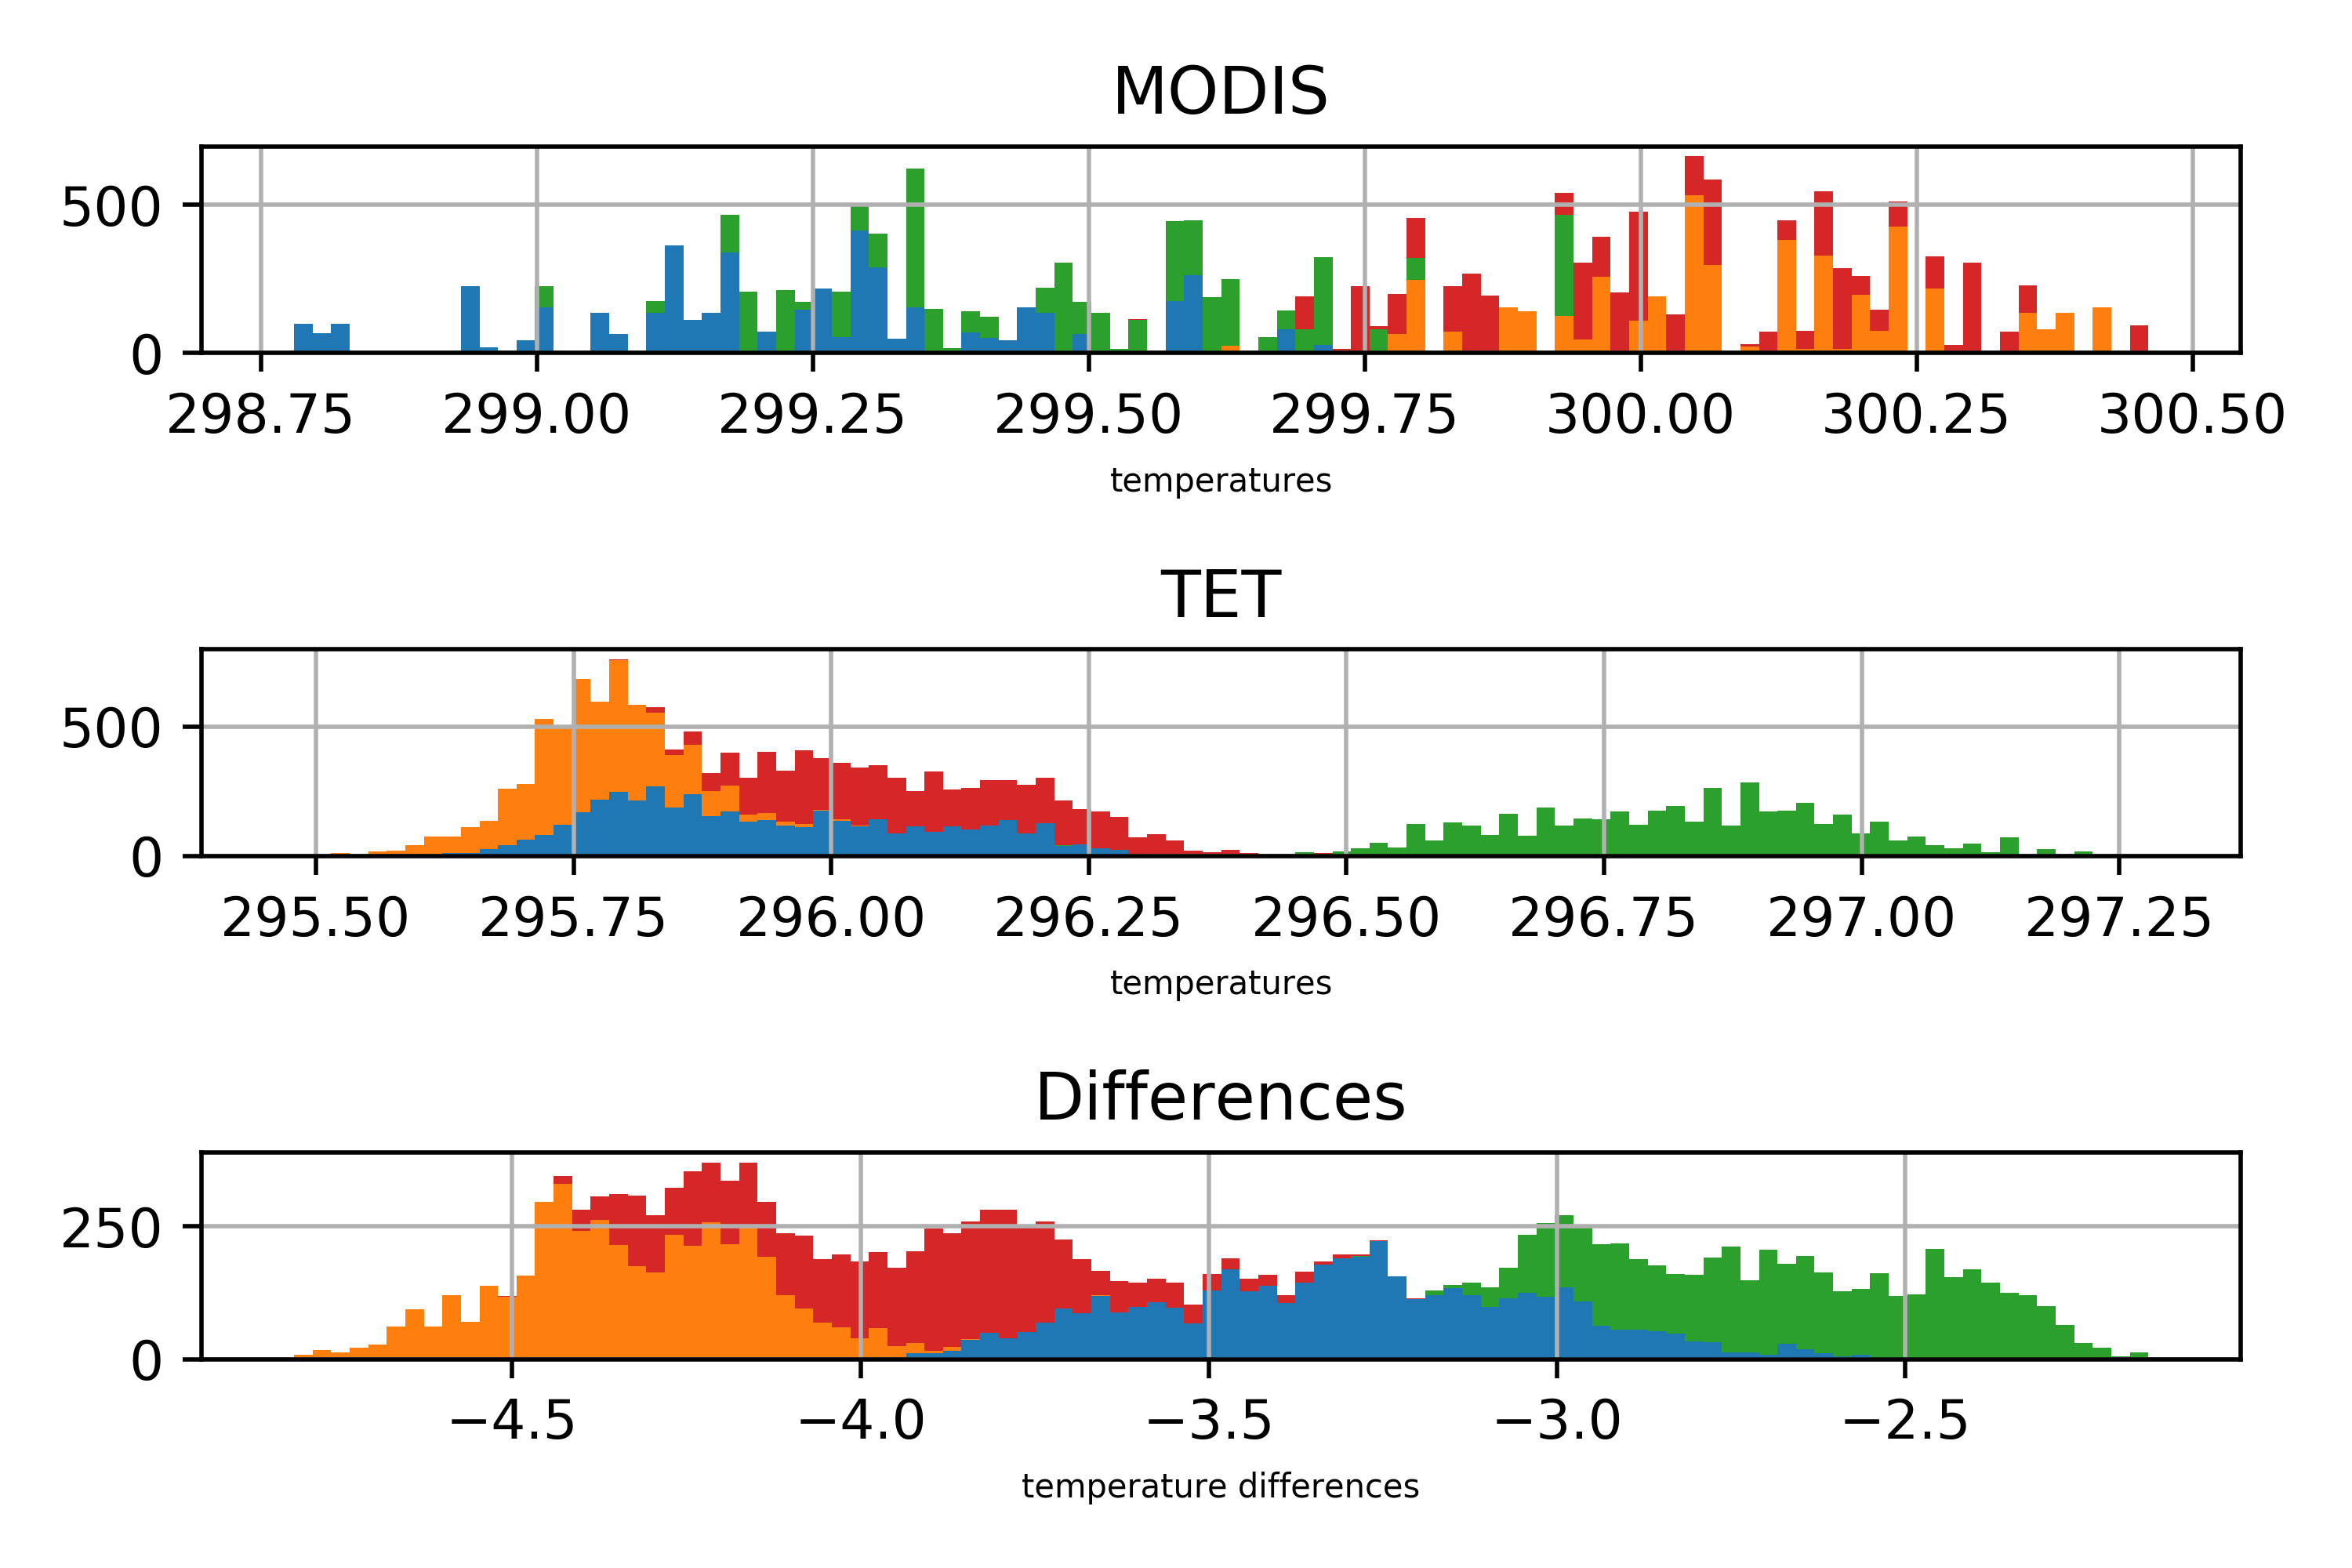
\includegraphics[width = 1.0\textwidth]{rect_all.png}
\caption{Histograms of all sub-areas of MODIS SST and TET-1 MIR band imageries with all the five scale factors. The red solid line in each histogram denotes the mean value and the red dashed line the standard deviation.}
\label{fig:rect_all_sc_all}
\end{figure}

\noindent Afterwards, in order to find the best scale factors for TET-1 MIR and TIR band imageries respectively, a time-serise analysis is performed. The results are shown in Figure \ref{fig:etna_sc_mir_tir}. The Figure \ref{fig:etna_bsc_tem} shows the best scale factor for each Etna scenes (the red solid line) and its corresponding temperature differences (the blue dashed line), which is also the minimal temperature differences. The ideal scale factor will be a constant over time, meaning constant scale factors can be applied to TET-1 MIR and TIR band imageries respectively, or it should be a periodic function of time. However, because of the unstable performance of the sensors, the influence of the space environment, the weather condition and so on, the temperature differences' behaviors of both TET-1 MIR and TIR band imageries are actually random. But it is still clear that for the TET-1 TIR band imagery, the scale factor 1.05 achieves the best performance that the temperature differences resulted from it are most close to zero. The Figure \ref{fig:etna_bsc_tir} also proves that, showing most of the TET-1 TIR band imageries has the best scale factor 1.05.\\

\noindent The situation for the TET-1 MIR band imagery is a bit complicated because the scale factor 1.10 and 1.15 have similar performances. Here scale factor 1.15 is selected artificially because of two points. On one hand, several scenes requires a scale factor higher than 1.15, namely 1.20. On the other hand, as we will present later, scale factor 1.15 shows a better transferability and performs better for scenes of other sites.\\

\begin{figure}[!htbp]
\centering
\subfigure[MIR band]{
\label{fig:etna_sc_mir}
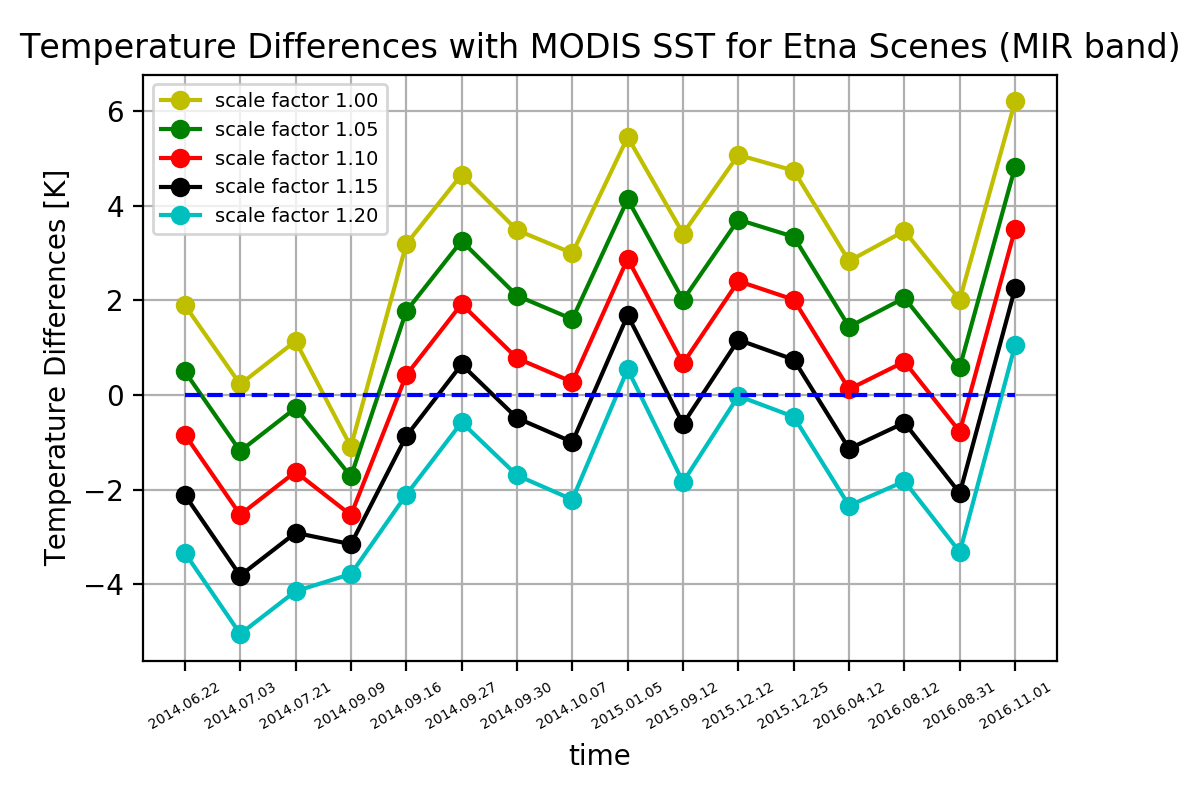
\includegraphics[width = 0.8\linewidth]{Etna_scf_mir.png}}
\hspace{0.5in}
\subfigure[TIR band]{
\label{fig:etna_sc_tir}
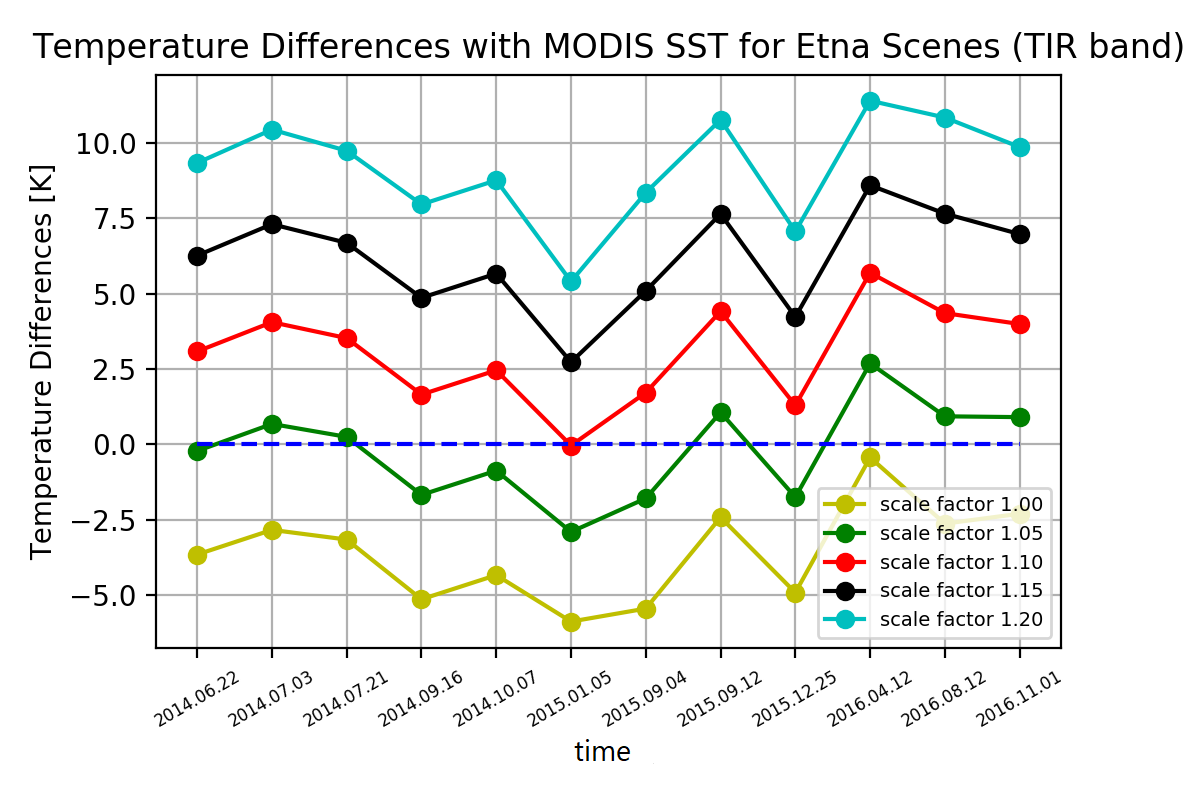
\includegraphics[width = 0.8\linewidth]{Etna_scf_tir.png}}
\caption{Temperature differences between TET-1 surface temperature maps and MODIS SST (Etna).}
\label{fig:etna_sc_mir_tir}
\end{figure}

\begin{figure}[!htbp]
\centering
\subfigure[MIR band]{
\label{fig:etna_bsc_mir}
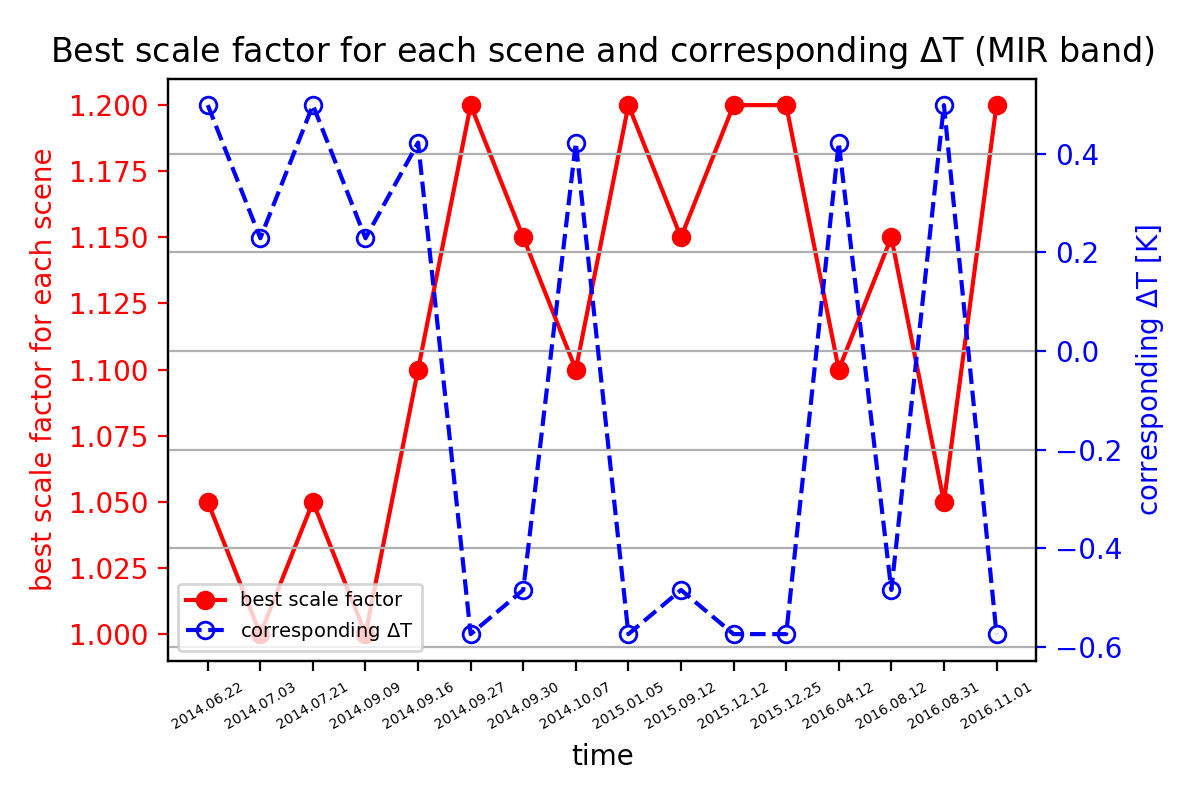
\includegraphics[width = 0.8\linewidth]{Etna_bsc&tem_mir.png}}
\hspace{0.5in}
\subfigure[TIR band]{
\label{fig:etna_bsc_tir}
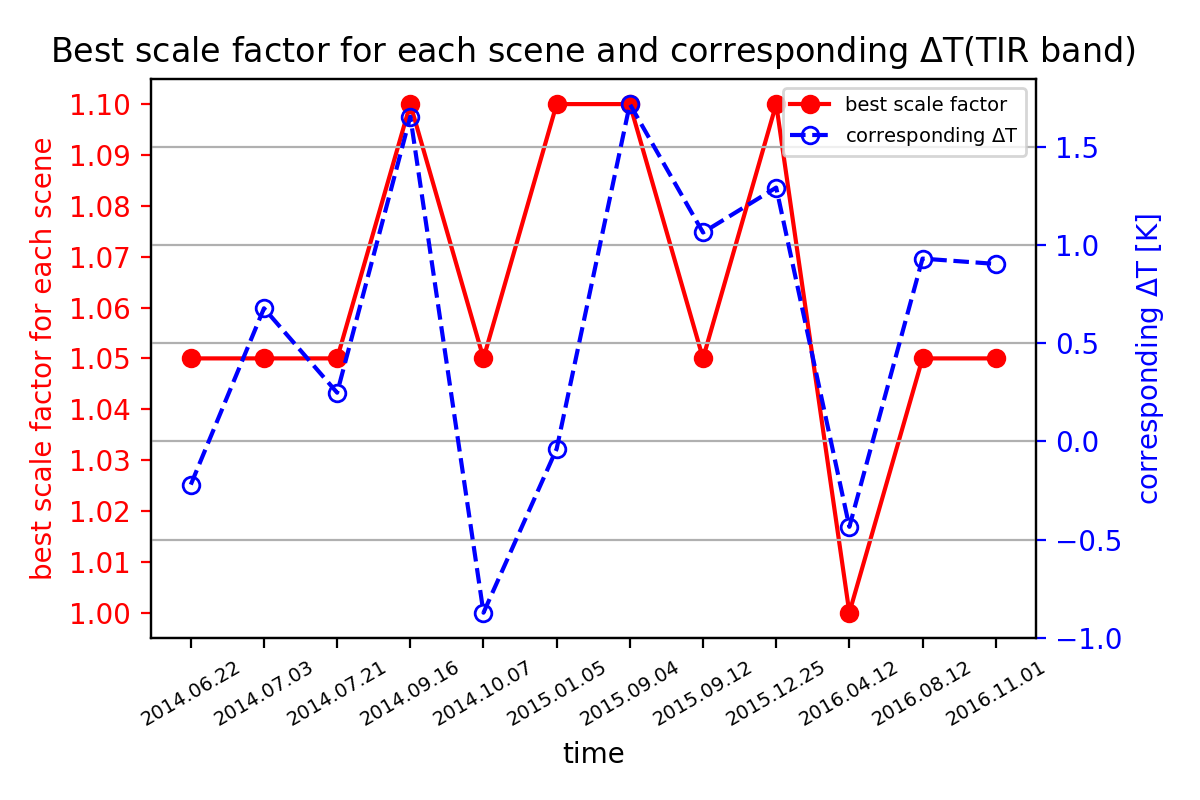
\includegraphics[width = 0.8\linewidth]{Etna_bsc&tem_tir.png}}
\caption{The best scale factors for each Etna scenes and its corresponding temperature differences. The red solid line is the best scale factor for each Etna scene. The blue dashed line is the minimal temperature differences resulted from that scale factor.}
\label{fig:etna_bsc_tem}
\end{figure}

\noindent As shown in Figure \ref{fig:etna_bsc&temComp}(a) that the temperature differences between MODIS SST and the surface temperature map in MIR band resulted from scale factor 1.15 are at most 4 K higher than the minimal temperature differences and at most of the time they differ only between 1 to 2 K. For surface temperature map in TIR band results from scale factor 1.05 differ from the smallest temperature differences at most 4 K as well.\\

\begin{figure}[!htbp]
\centering
\subfigure[MIR band]{
\label{fig:etna_bsc&temComp_mir}
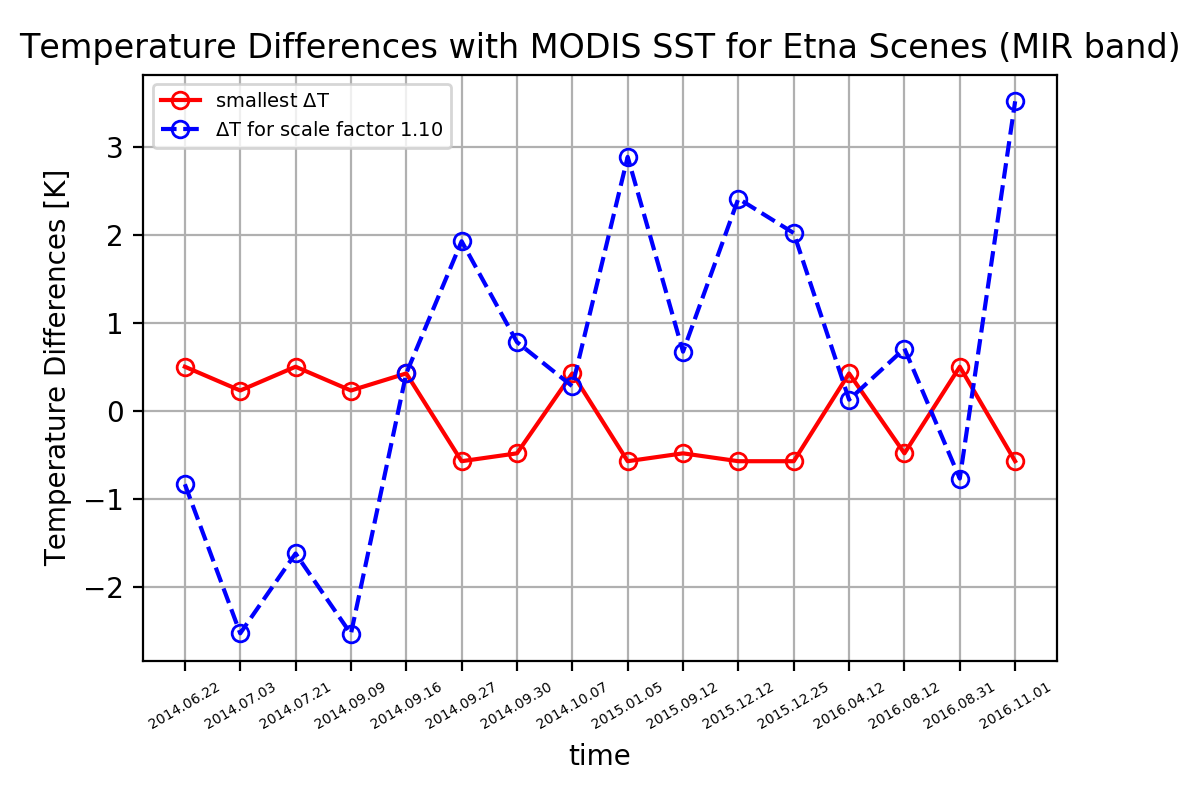
\includegraphics[width = 0.8\linewidth]{Etna_bsc&temCom_mir.png}}
\hspace{0.5in}
\subfigure[TIR band]{
\label{fig:etna_bsc&temComp_tir}
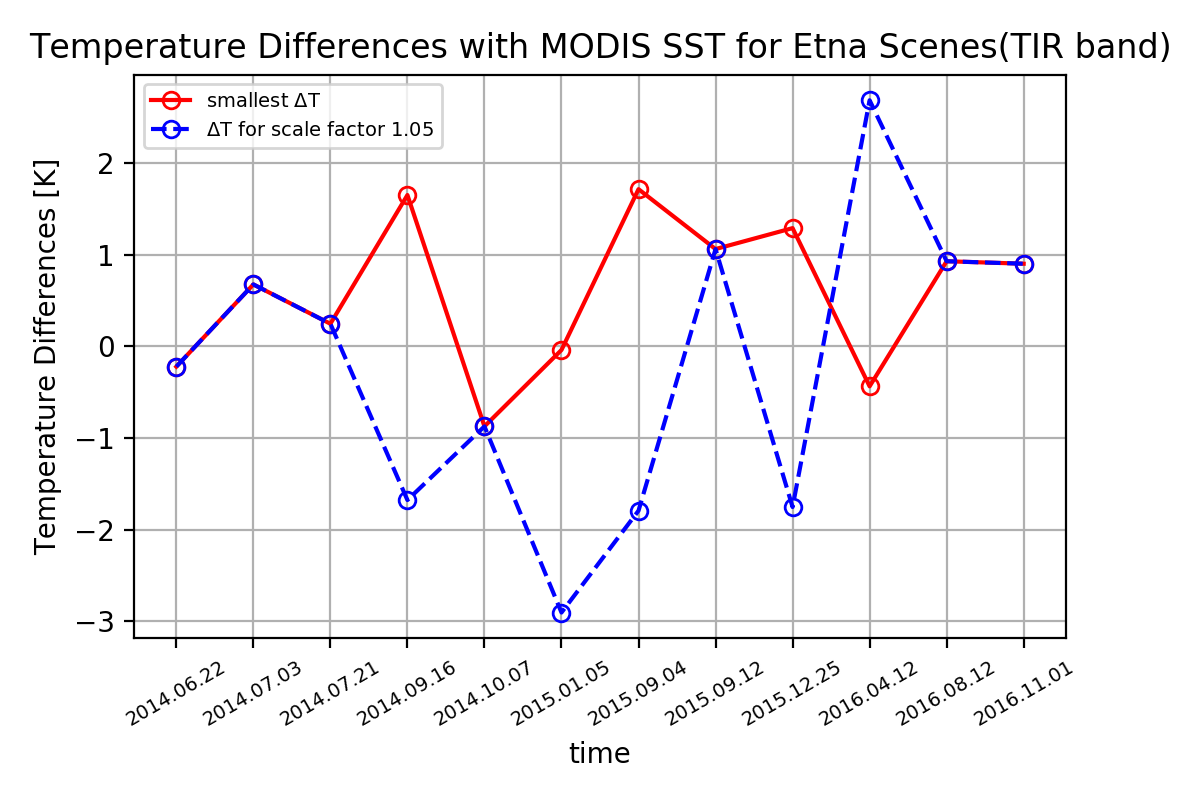
\includegraphics[width = 0.8\linewidth]{Etna_bsc&temCom_tir.png}}
\caption{The minimal temperature differences and the temperature differences resulted from scale factor 1.15 and scale factor 1.05. The red solid line is the minimal temperature differences for each Etna scene. The blue dashed line is the temperature differences resulted from the selected scale factors for MIR and TIR band imageries, scale factor 1.15 (upper) and scale factor 1.05 (lower), respectively.}
\label{fig:etna_bsc&temComp}
\end{figure}

%-----------------------------------
%	SUBSECTION 3
%-----------------------------------

% \subsection{Calibrations}

%-----------------------------------
%	SUBSECTION 3
%-----------------------------------
\subsection{transferability test (SST)}
The best scale factors for the TET-1 MIR and TIR band imageries are selected as 1.15 and 1.05 respectively in the previous section. But they are selected based on TET-1 imageries of one site only. Before applying them to other imageries, their transferability should be tested to see whether the scale factors got from Etna scenes are suitable for other sites as well. Consequently, three other scenes of Etna, one scene of Portugal and two scenes of Demmin are used as test scenes to validate the chosen scale factors.\\

\begin{figure}[!htbp]
\centering
\subfigure[Portugal]{
\label{fig:Portugal}
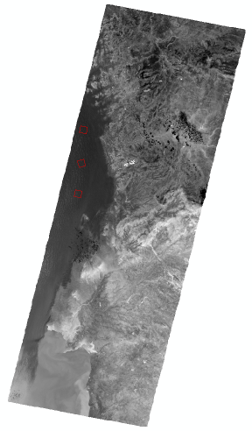
\includegraphics[width = 0.4\linewidth]{Portugal.png}}
\vspace{0.5in}
\subfigure[Demmin]{
\label{fig:Demmin}
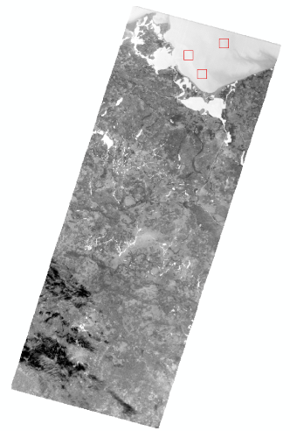
\includegraphics[width = 0.4\linewidth]{Demmin.png}}
\caption{The example figures of Portugal and Demmin. The red rectangles represent the selected sub-areas.}
\label{fig:portugal&demmin}
\end{figure}

\noindent Besides the chosen scale factor 1.15 for MIR band imagery and 1.05 for TIR band imagery, the performances of scale factor 1.10 and 1.20 are also presented for the MIR band imagery as comparison and for TIR band imagery, the performances of scale factor 1.00 and 1.10 are displayed as well for the same purpose. As shown in Figure \ref{fig:SST_test}, scale factor 1.15 for MIR band imagery and scale factor 1.05 for TIR band imagery are not always optimal scale factors for each scene, however, they demonstrate better performances than the other scale factors over time and sites.\\

\begin{figure}[!htbp]
\centering
\subfigure[MIR band]{
\label{fig:SST_test_mir}
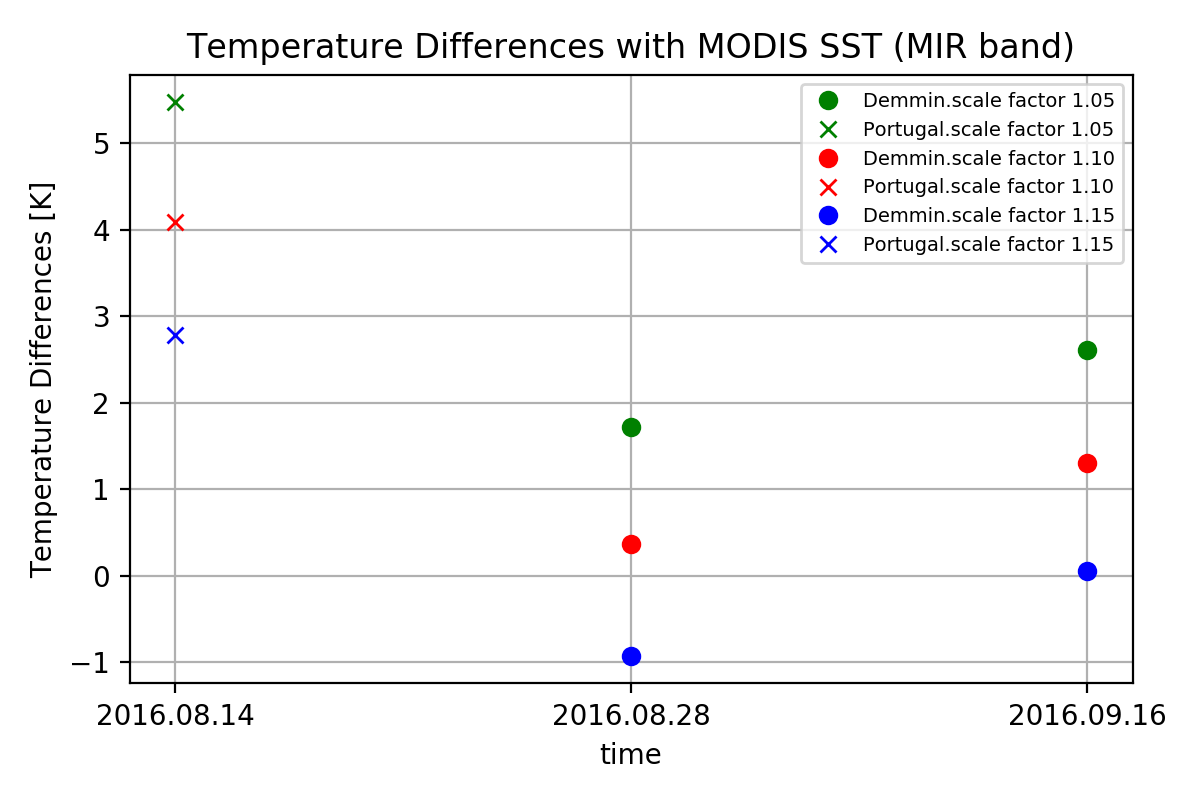
\includegraphics[width = 0.8\linewidth]{sst_test&comp_mir.png}}
\hspace{0.5in}
\subfigure[TIR band]{
\label{fig:SST_test_tir}
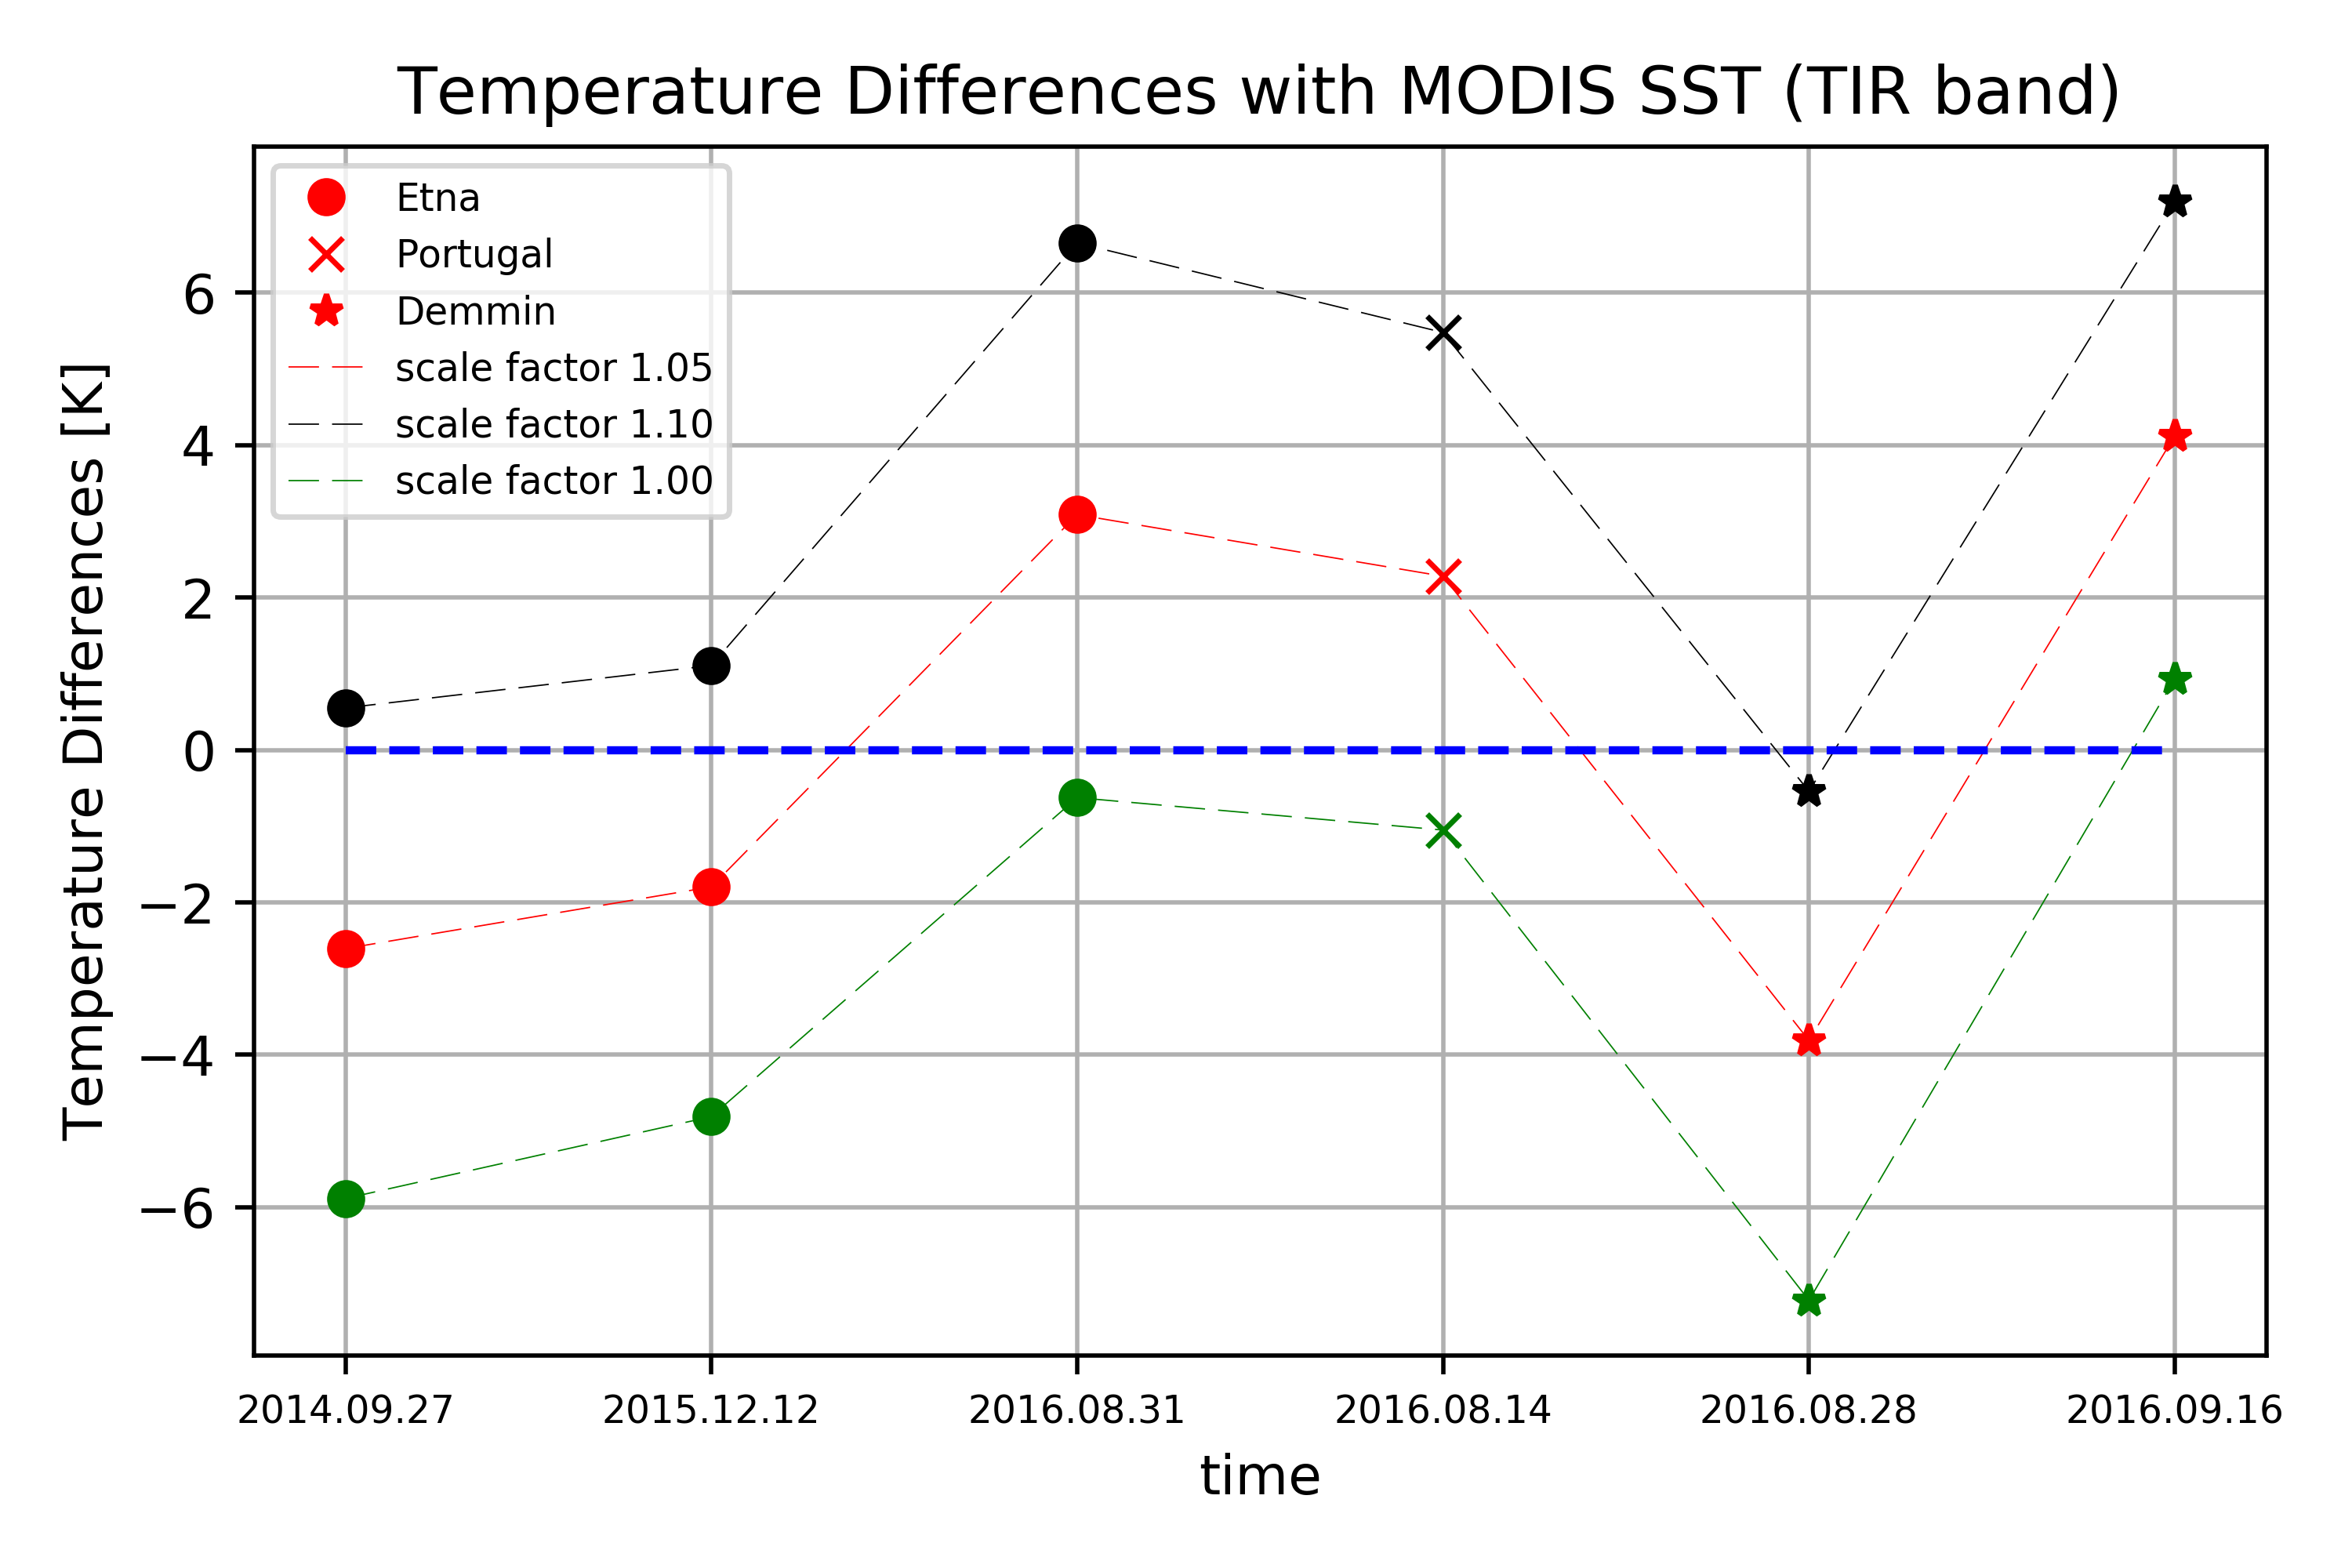
\includegraphics[width = 0.8\linewidth]{sst_test&comp_tir.png}}
\caption{Transferability test: temperature differences between TET-1 surface temperature maps and MODIS SST.}
\label{fig:SST_test}
\end{figure}

%-----------------------------------
%	SUBSECTION 4
%-----------------------------------

\subsection{Results comparison with MODIS LST and calibration}
The similar comparison is done between the temperature results from MITIP and MODIS LST over the scenes of the test site Libya-1. However, the emissivities of different land features vary a lot. So the problem that which band of the emissivity maps should be used matters. The temperature maps of MITIP resulted from different emissivity maps are presented as follows.\\

\begin{figure}[!htbp]
\centering
\subfigure[Temperature (Libya-1) with different emissivities]{
\label{fig:emi_Libya_1}
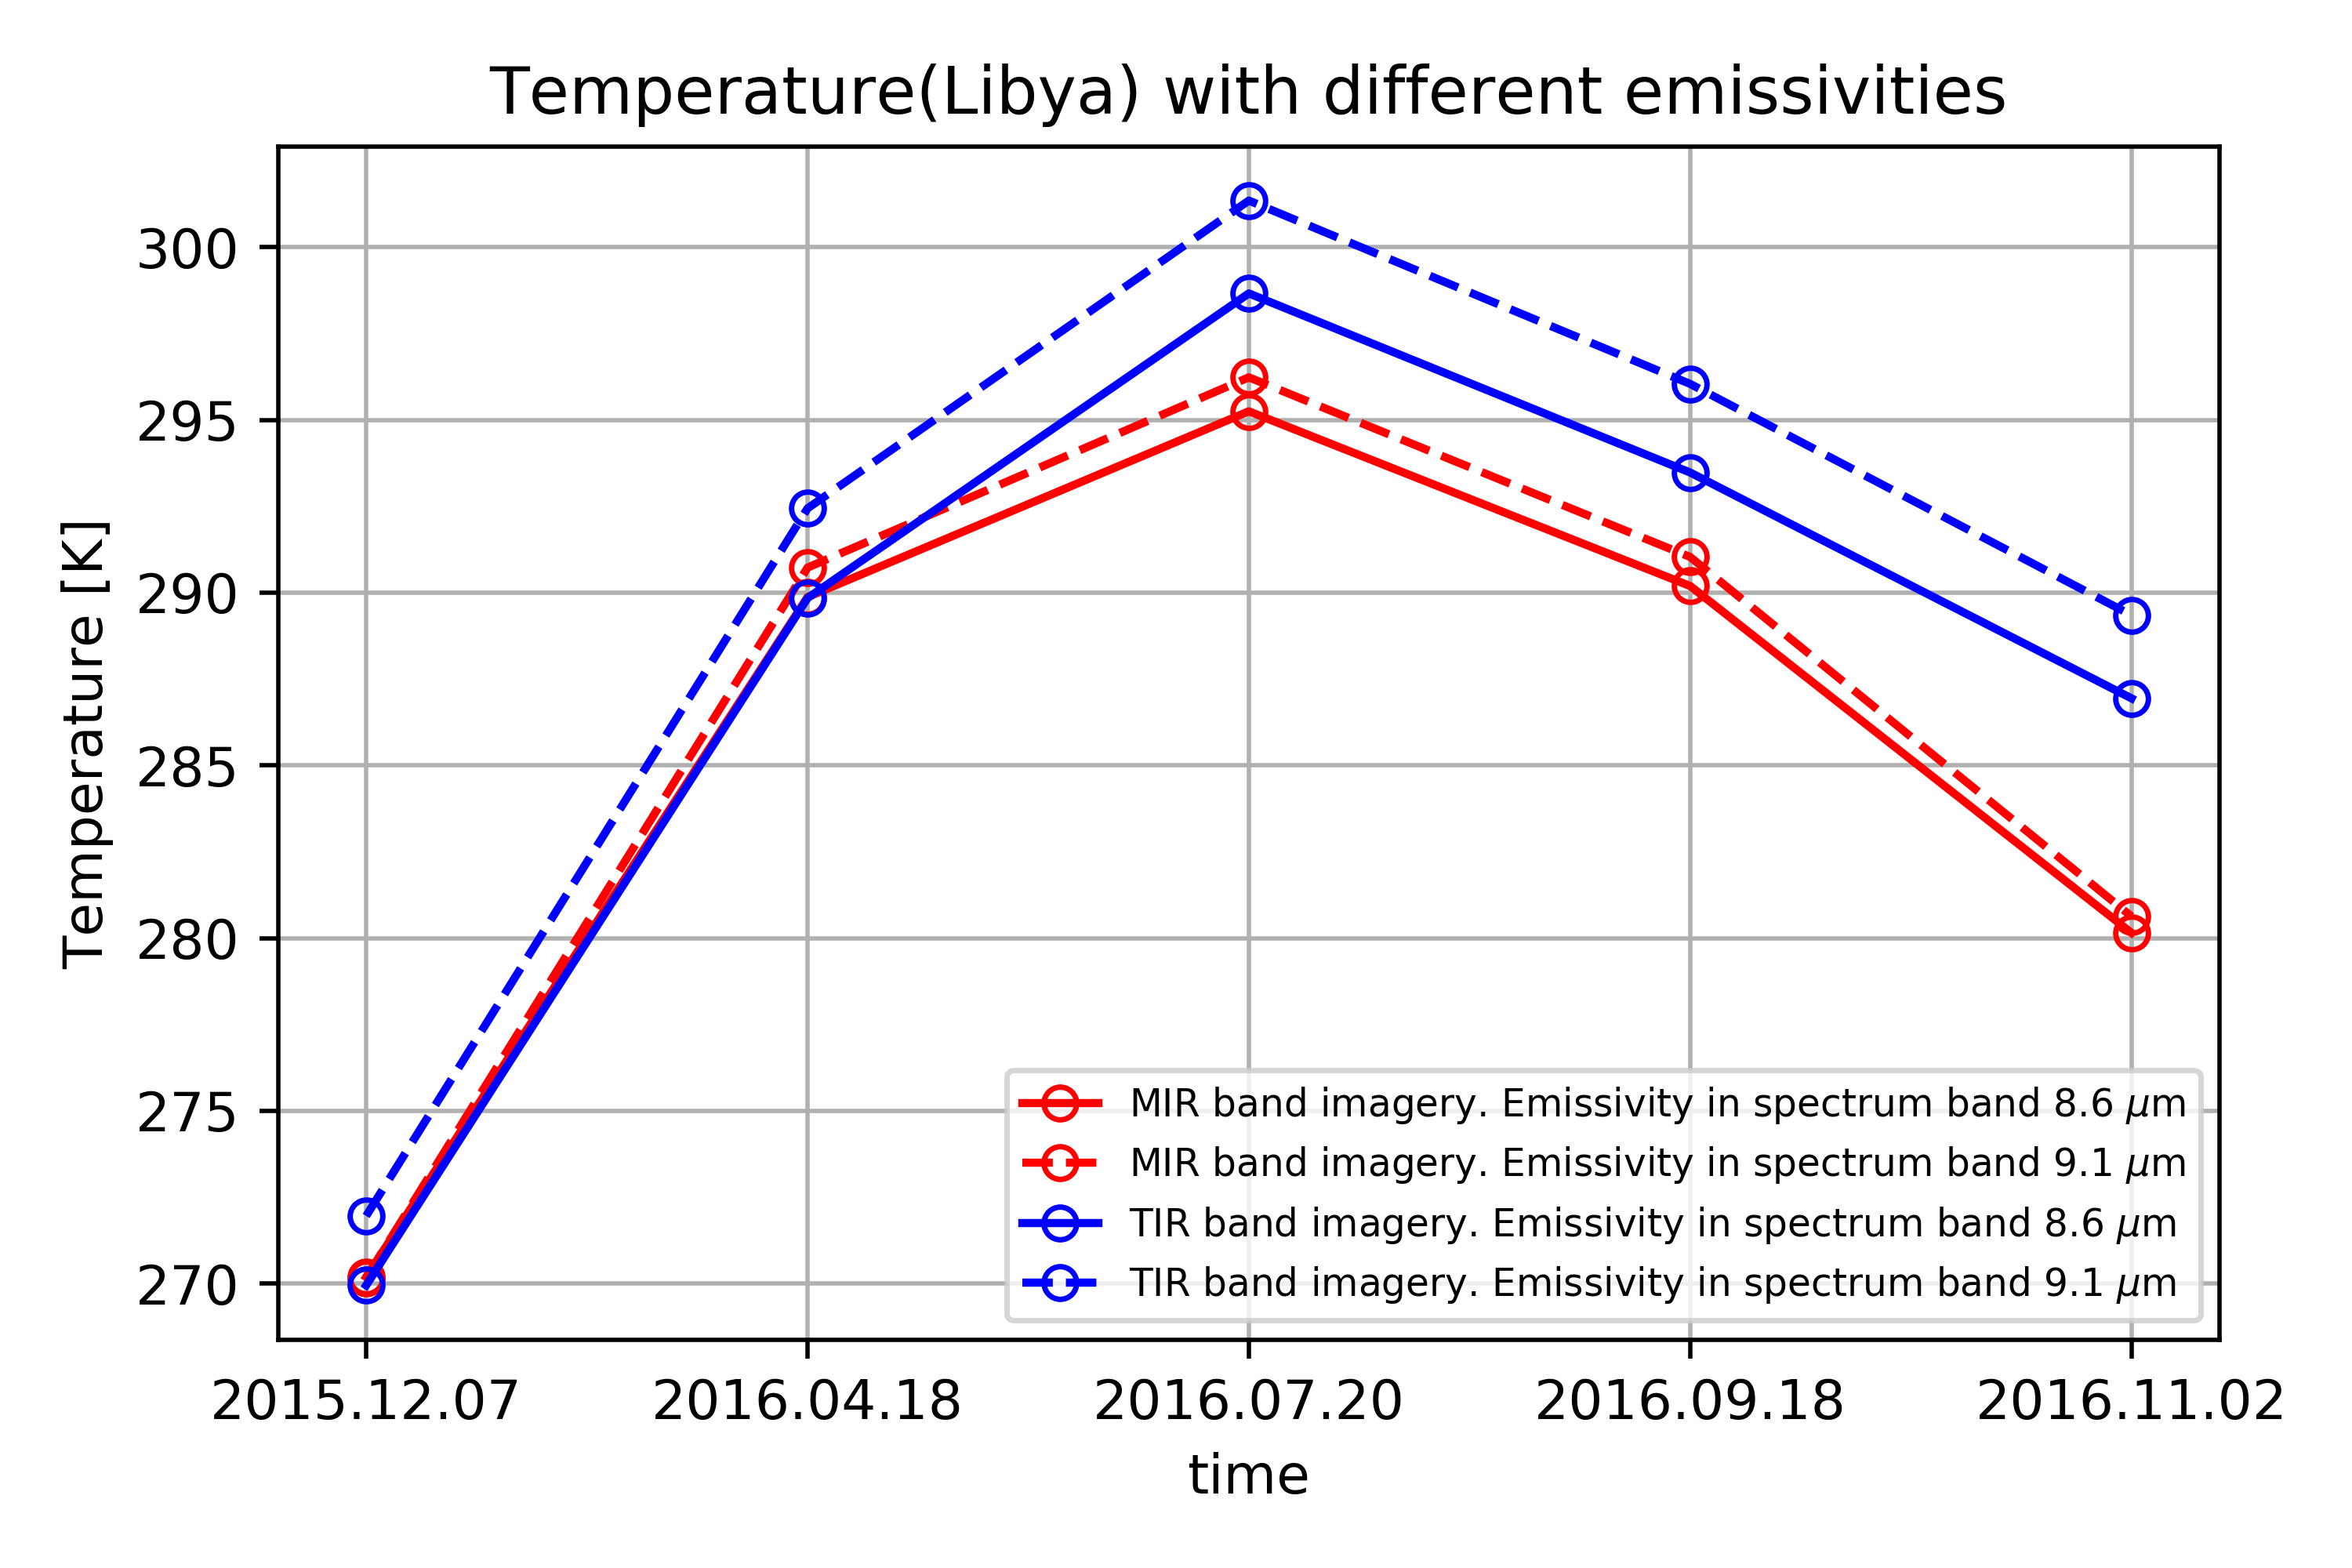
\includegraphics[width = 0.8\linewidth]{diff_emi1_Lybia.png}}
\hspace{0.5in}
\subfigure[Temperature differences (Libya-1) with different emissivities]{
\label{fig:emi_Libya_2}
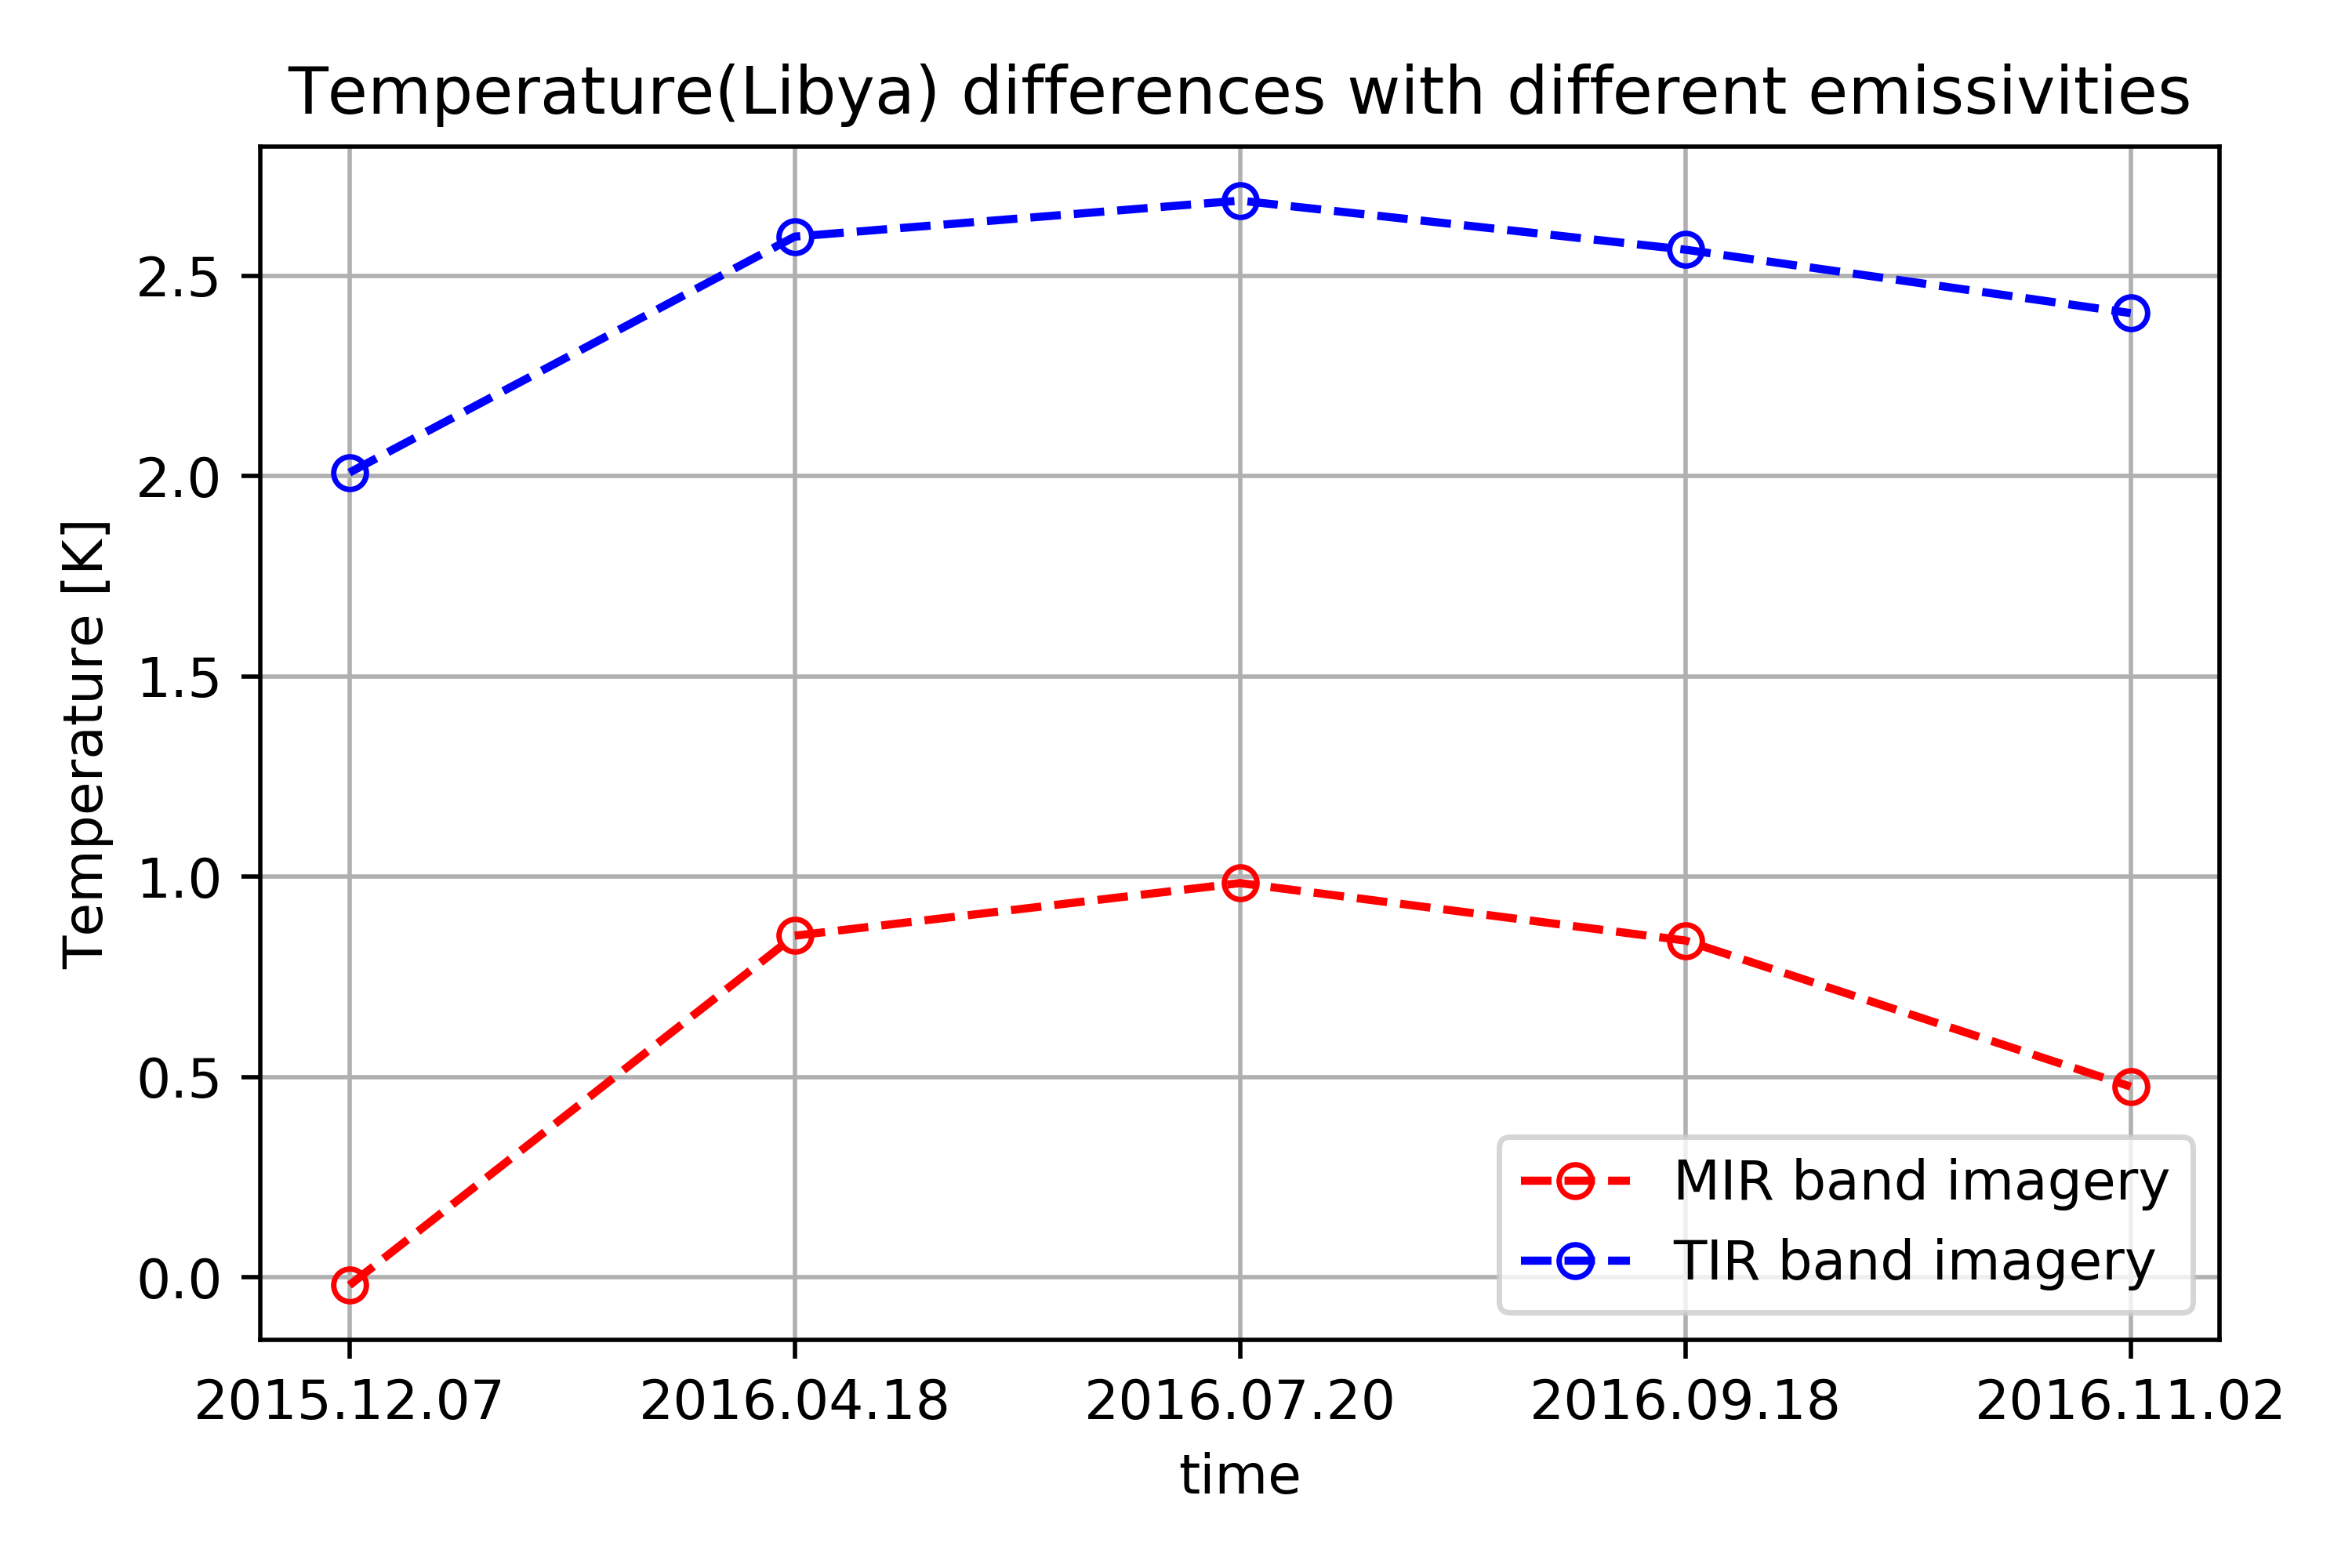
\includegraphics[width = 0.8\linewidth]{diff_emi2_Lybia.png}}
\caption{The effect of different emissivities on the surface temperature maps from MITIP.}
\label{fig:diff_emi_Lybia}
\end{figure}

\noindent from the Figure \ref{fig:diff_emi_Lybia} it is clear that different emissivities maps have great influence on the temperature maps from MITIP.  Figure \ref{fig:emi_Libya_2} shows that the temperature differences in TET-1 TIR band imageries are much higher than the temperature differences in the MIR band imageries both caused by the emissivity maps. Consequently, the focus will be laid on the TET-1 TIR band imageries.\\

\begin{figure}[!htbp]
\centering
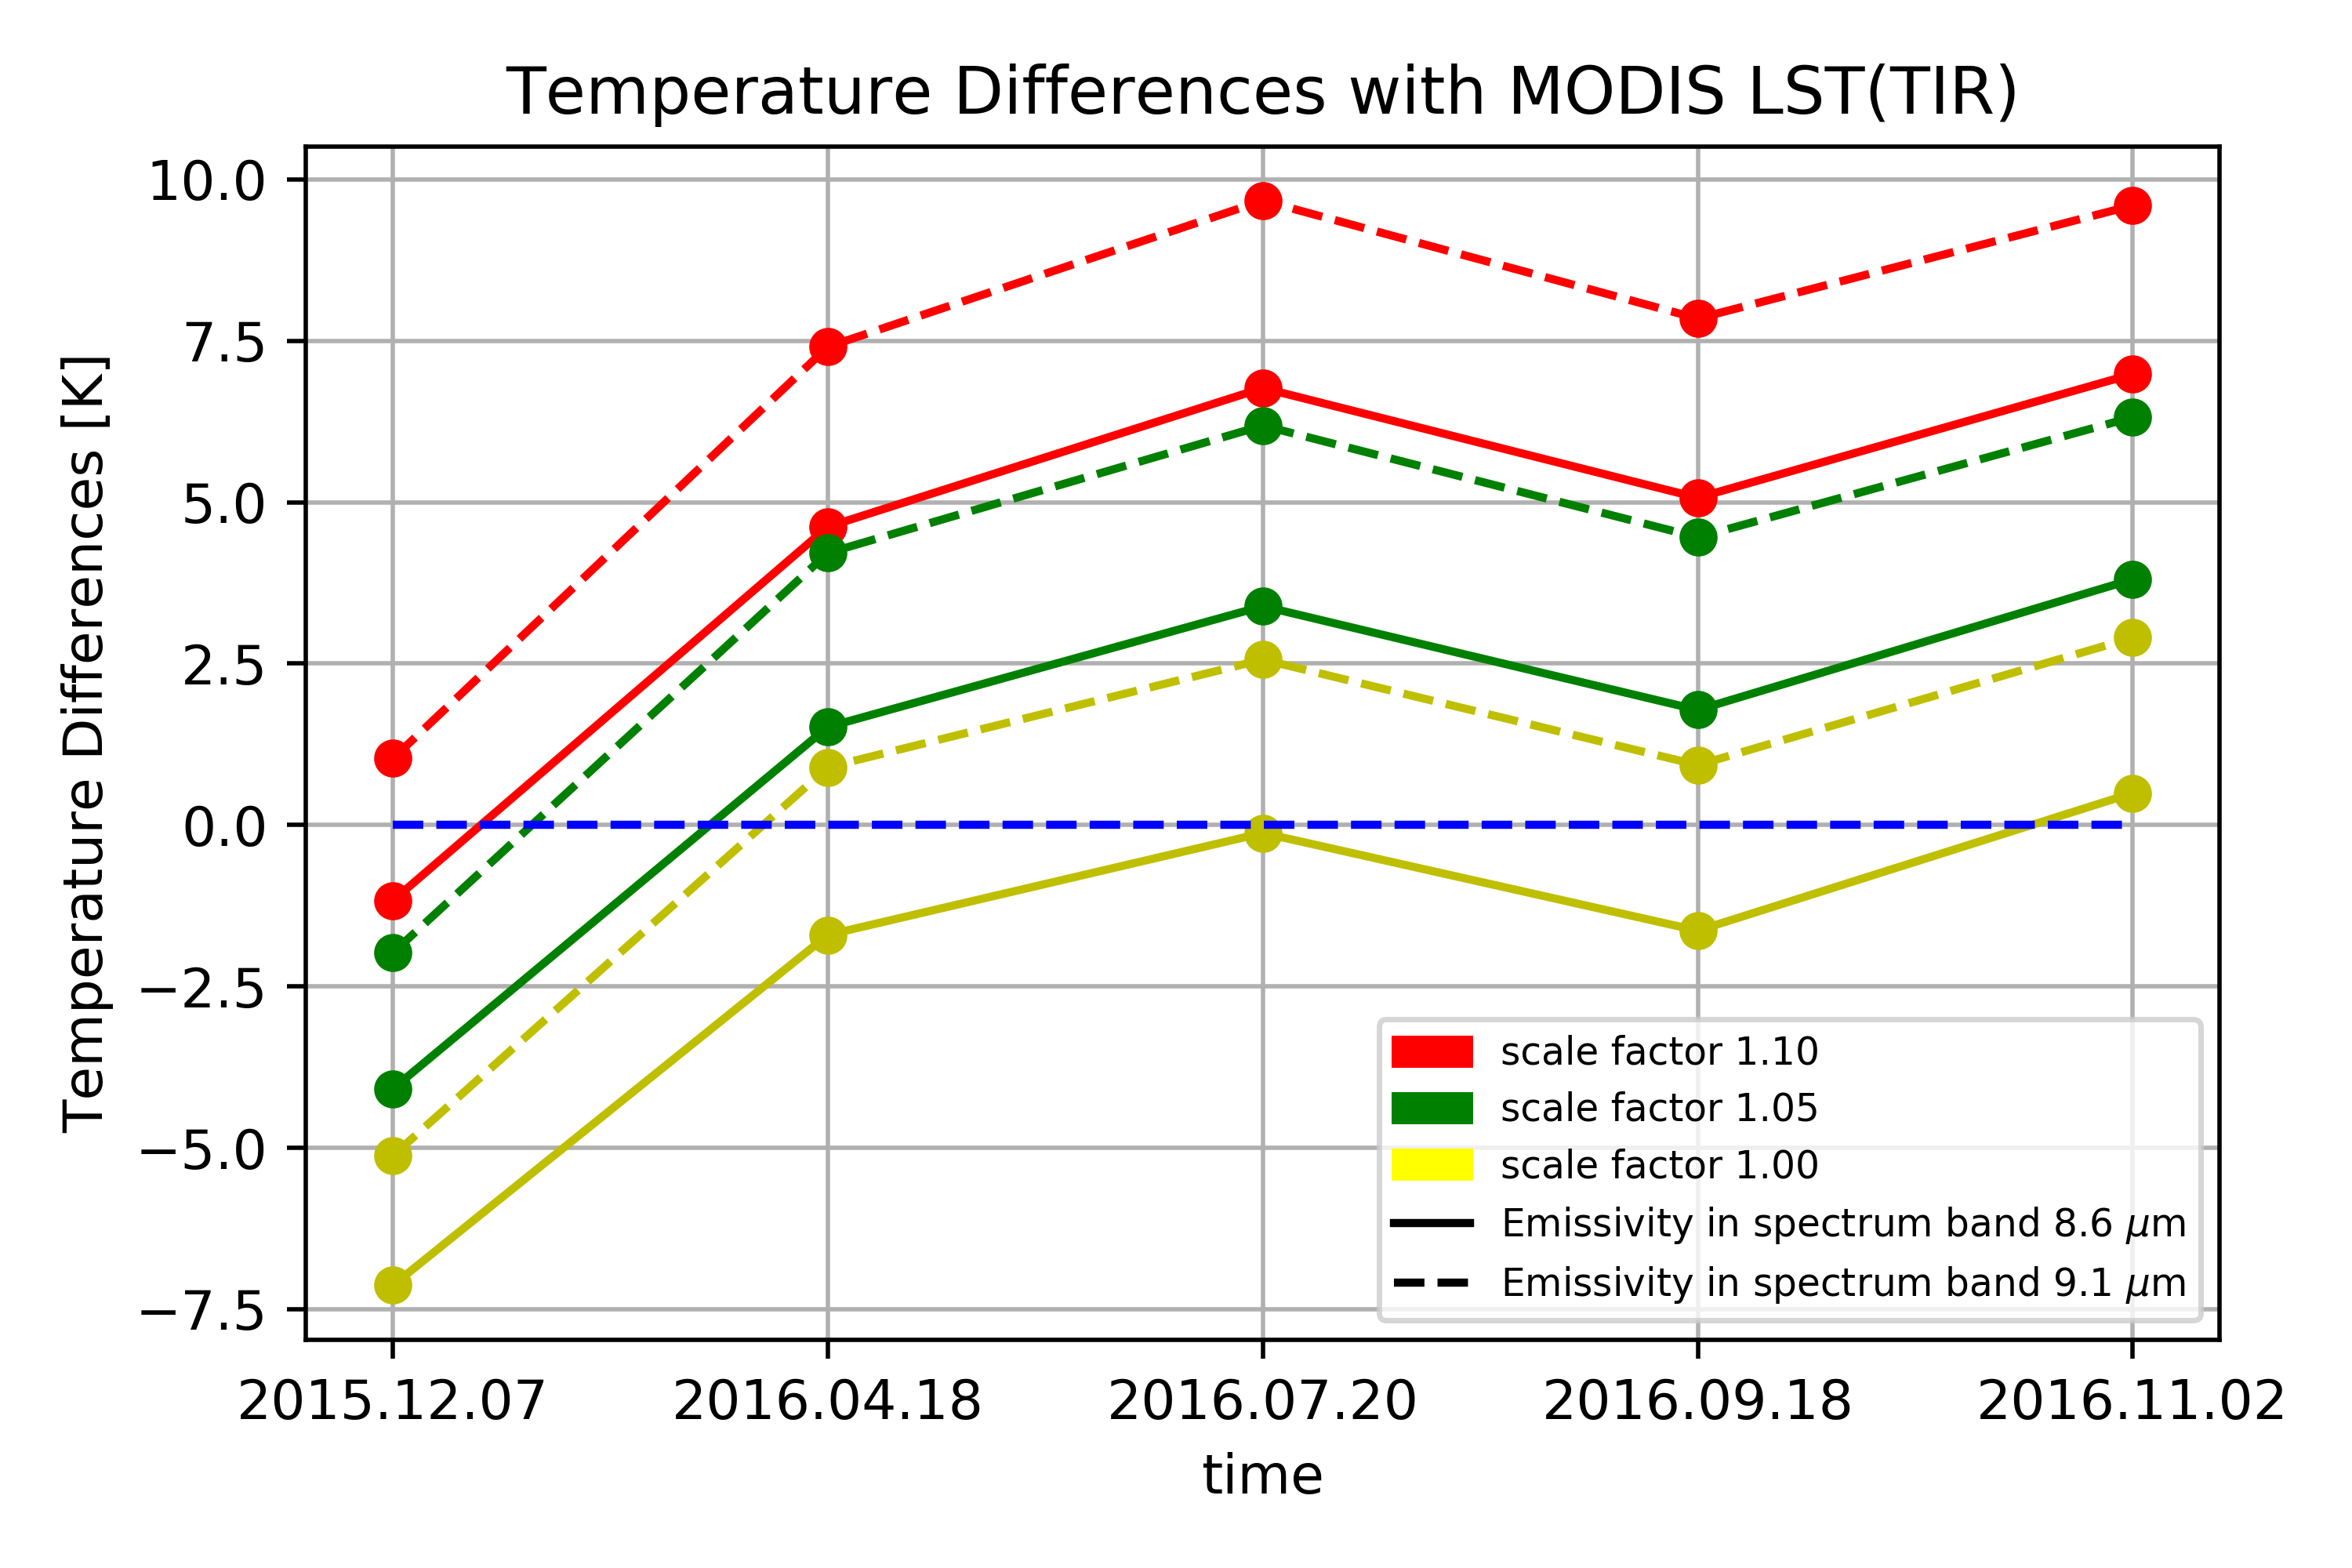
\includegraphics[width = 0.8\textwidth]{diff_emi_tir1.png}
\caption{Temperature differences (Lybia-1) between the surface temperature maps in TIR band and MODIS LST.}
\label{fig:diff_emi_tir1}
\end{figure}

\noindent Figure \ref{fig:diff_emi_tir1} shows that the emissivity maps have effects comparable with the effects of the scale factors and it is clear that with the same scale factor, the temperature differences in TIR band resulted from emissivity map in 8.6 $\mu$m are much lower than these from the emissivity in band 9.1 $\mu$m. The temperature differences in MIR band with different emissivity maps also prove that as shown in Figure \ref{fig:diff_emi_mir1}.\\

\begin{figure}[!htbp]
\centering
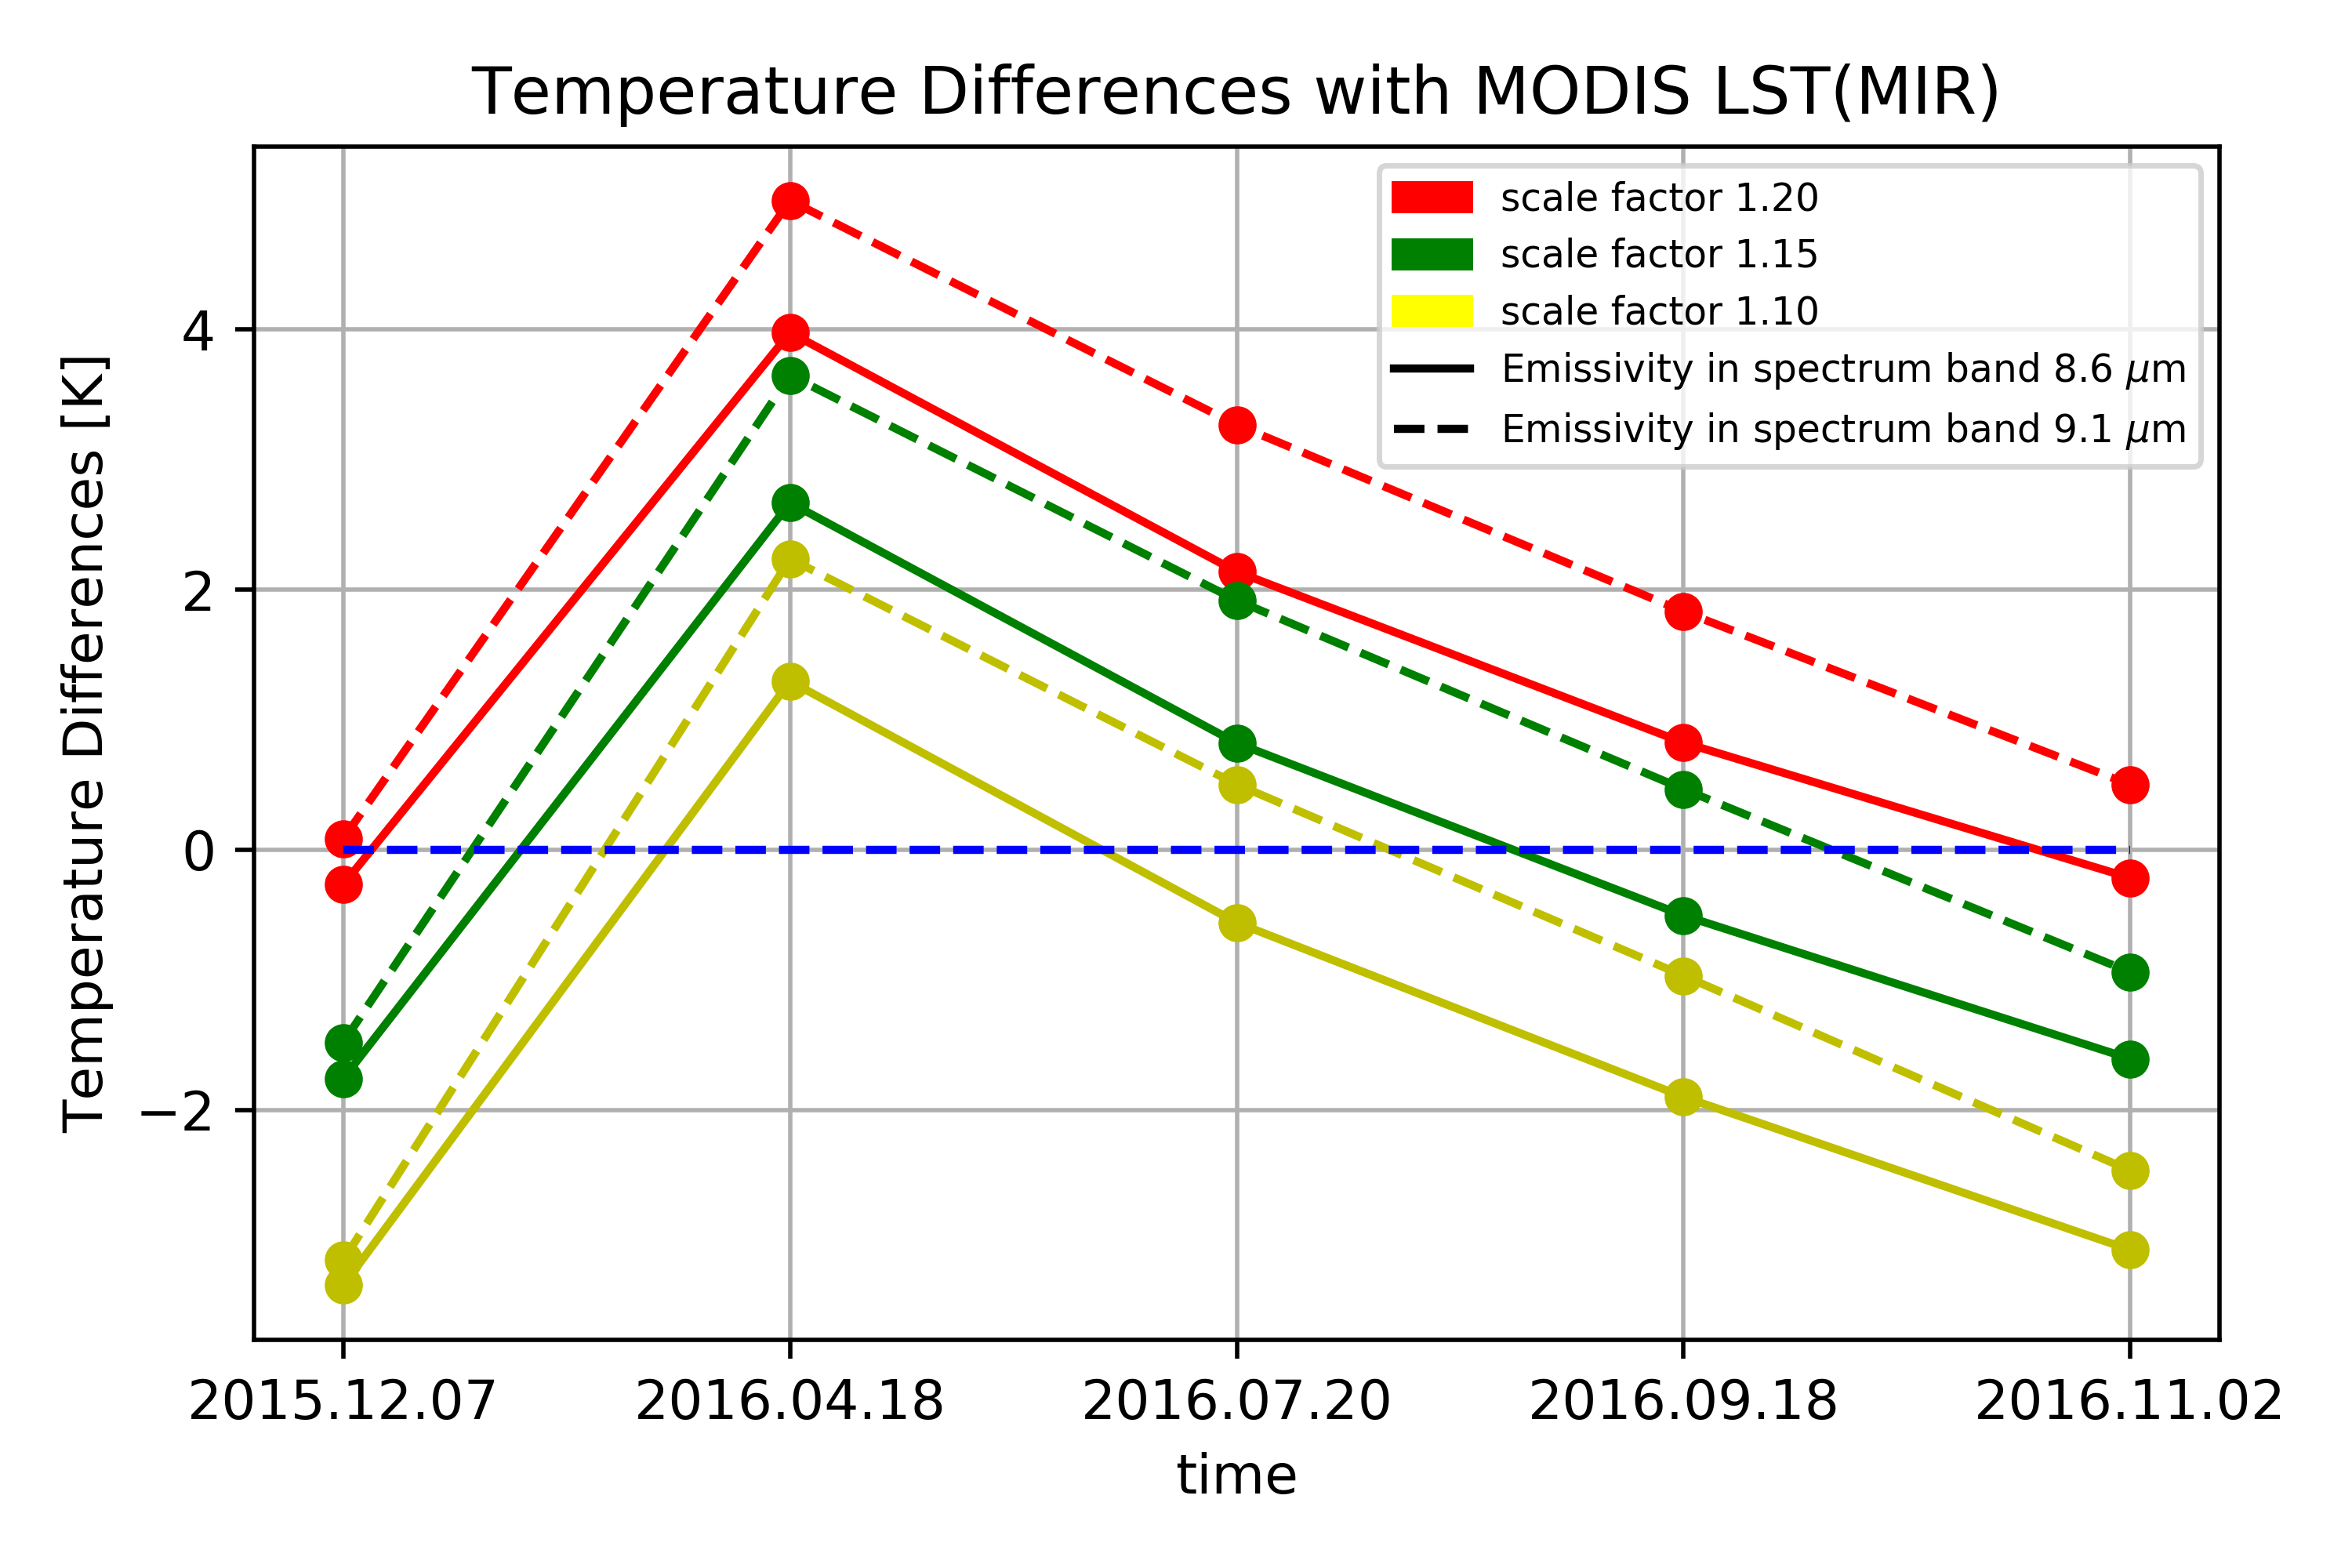
\includegraphics[width = 0.8\textwidth]{diff_emi_mir1.png}
\caption{Temperature differences (Lybia-1) between the surface temperature maps in MIR band and MODIS LST.}
\label{fig:diff_emi_mir1}
\end{figure}

\noindent Concentrate on one certain scale factor, as shown in Figure \ref{fig:diff_emi_Lybia2}, we can see that using the emissivity map with spectral band 9.1 $\mu$m, the temperature differences between the surface temperature maps from MITIP and MODIS LST is much higher than those using the emissivity map with spectral band 8.6 $\mu$m. Besides, in order to keep consistent with the comparison with the MODIS SST, the emissivity map with spectral band 8.6 $\mu$m will be reminded in use.\\

\begin{figure}[!htbp]
\centering
\subfigure[MIR band]{
\label{fig:diff_emi_mir2}
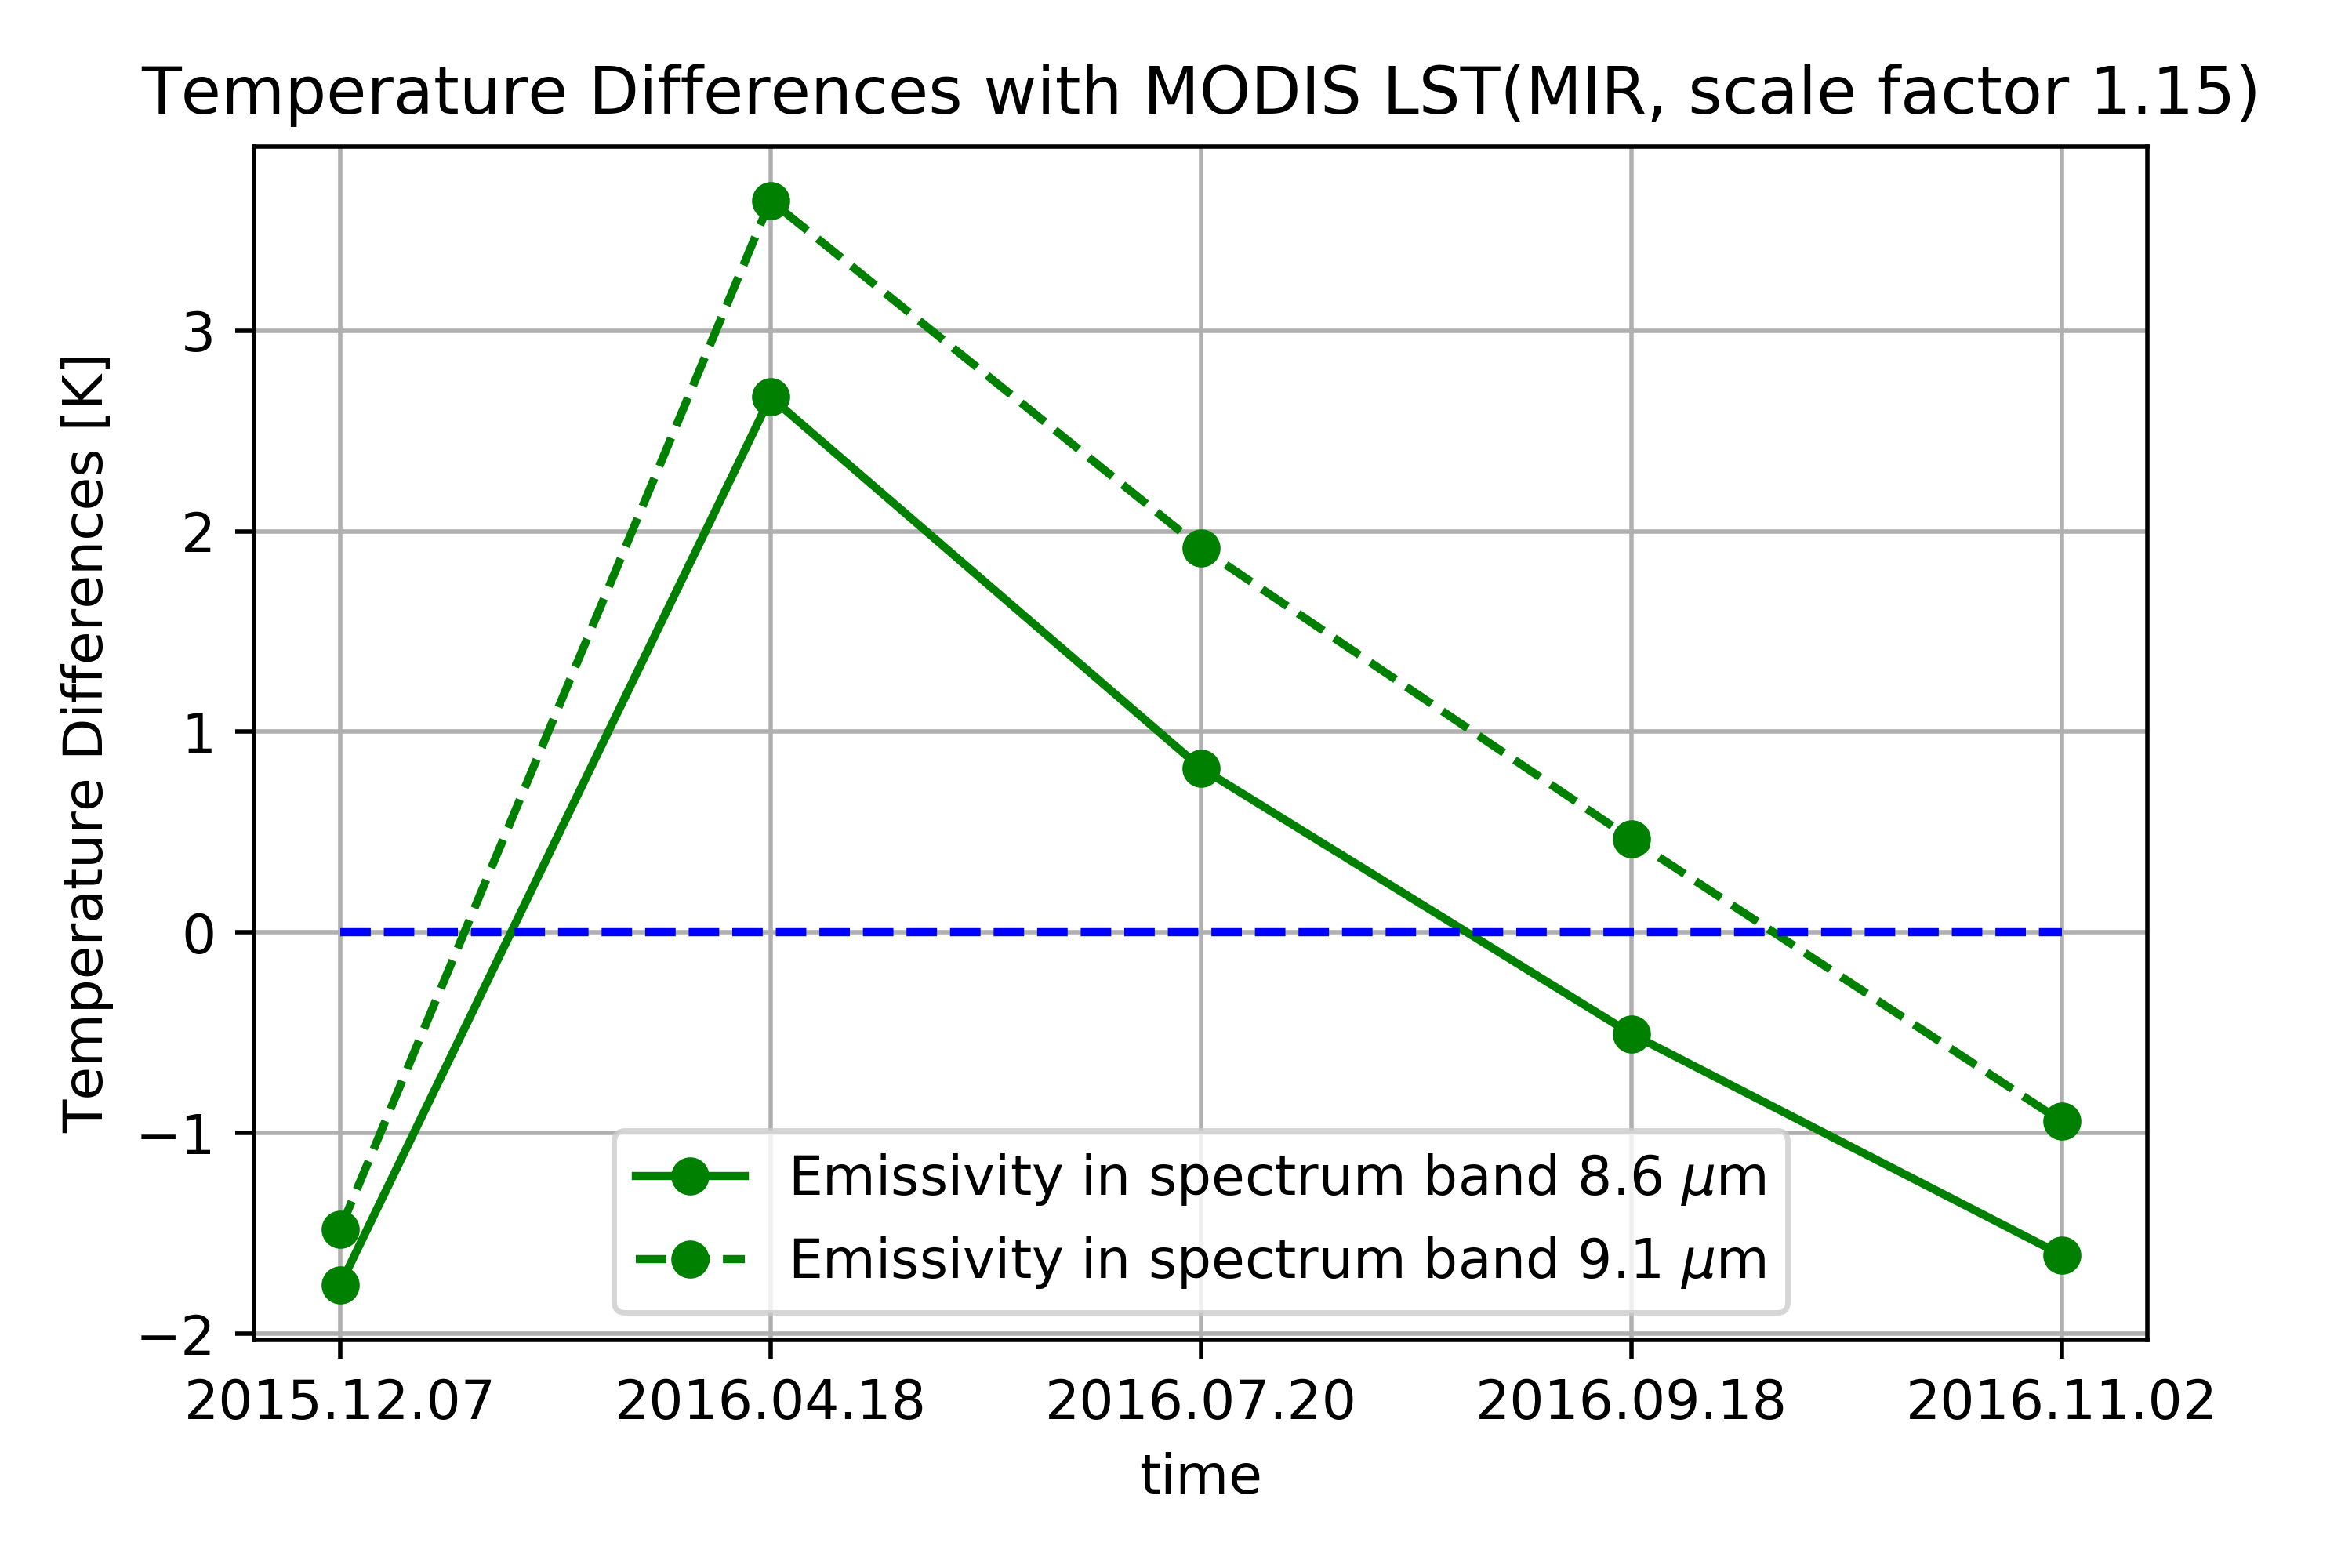
\includegraphics[width = 0.8\linewidth]{diff_emi_mir2.png}}
\hspace{0.5in}
\subfigure[TIR band]{
\label{fig:diff_emi_tir2}
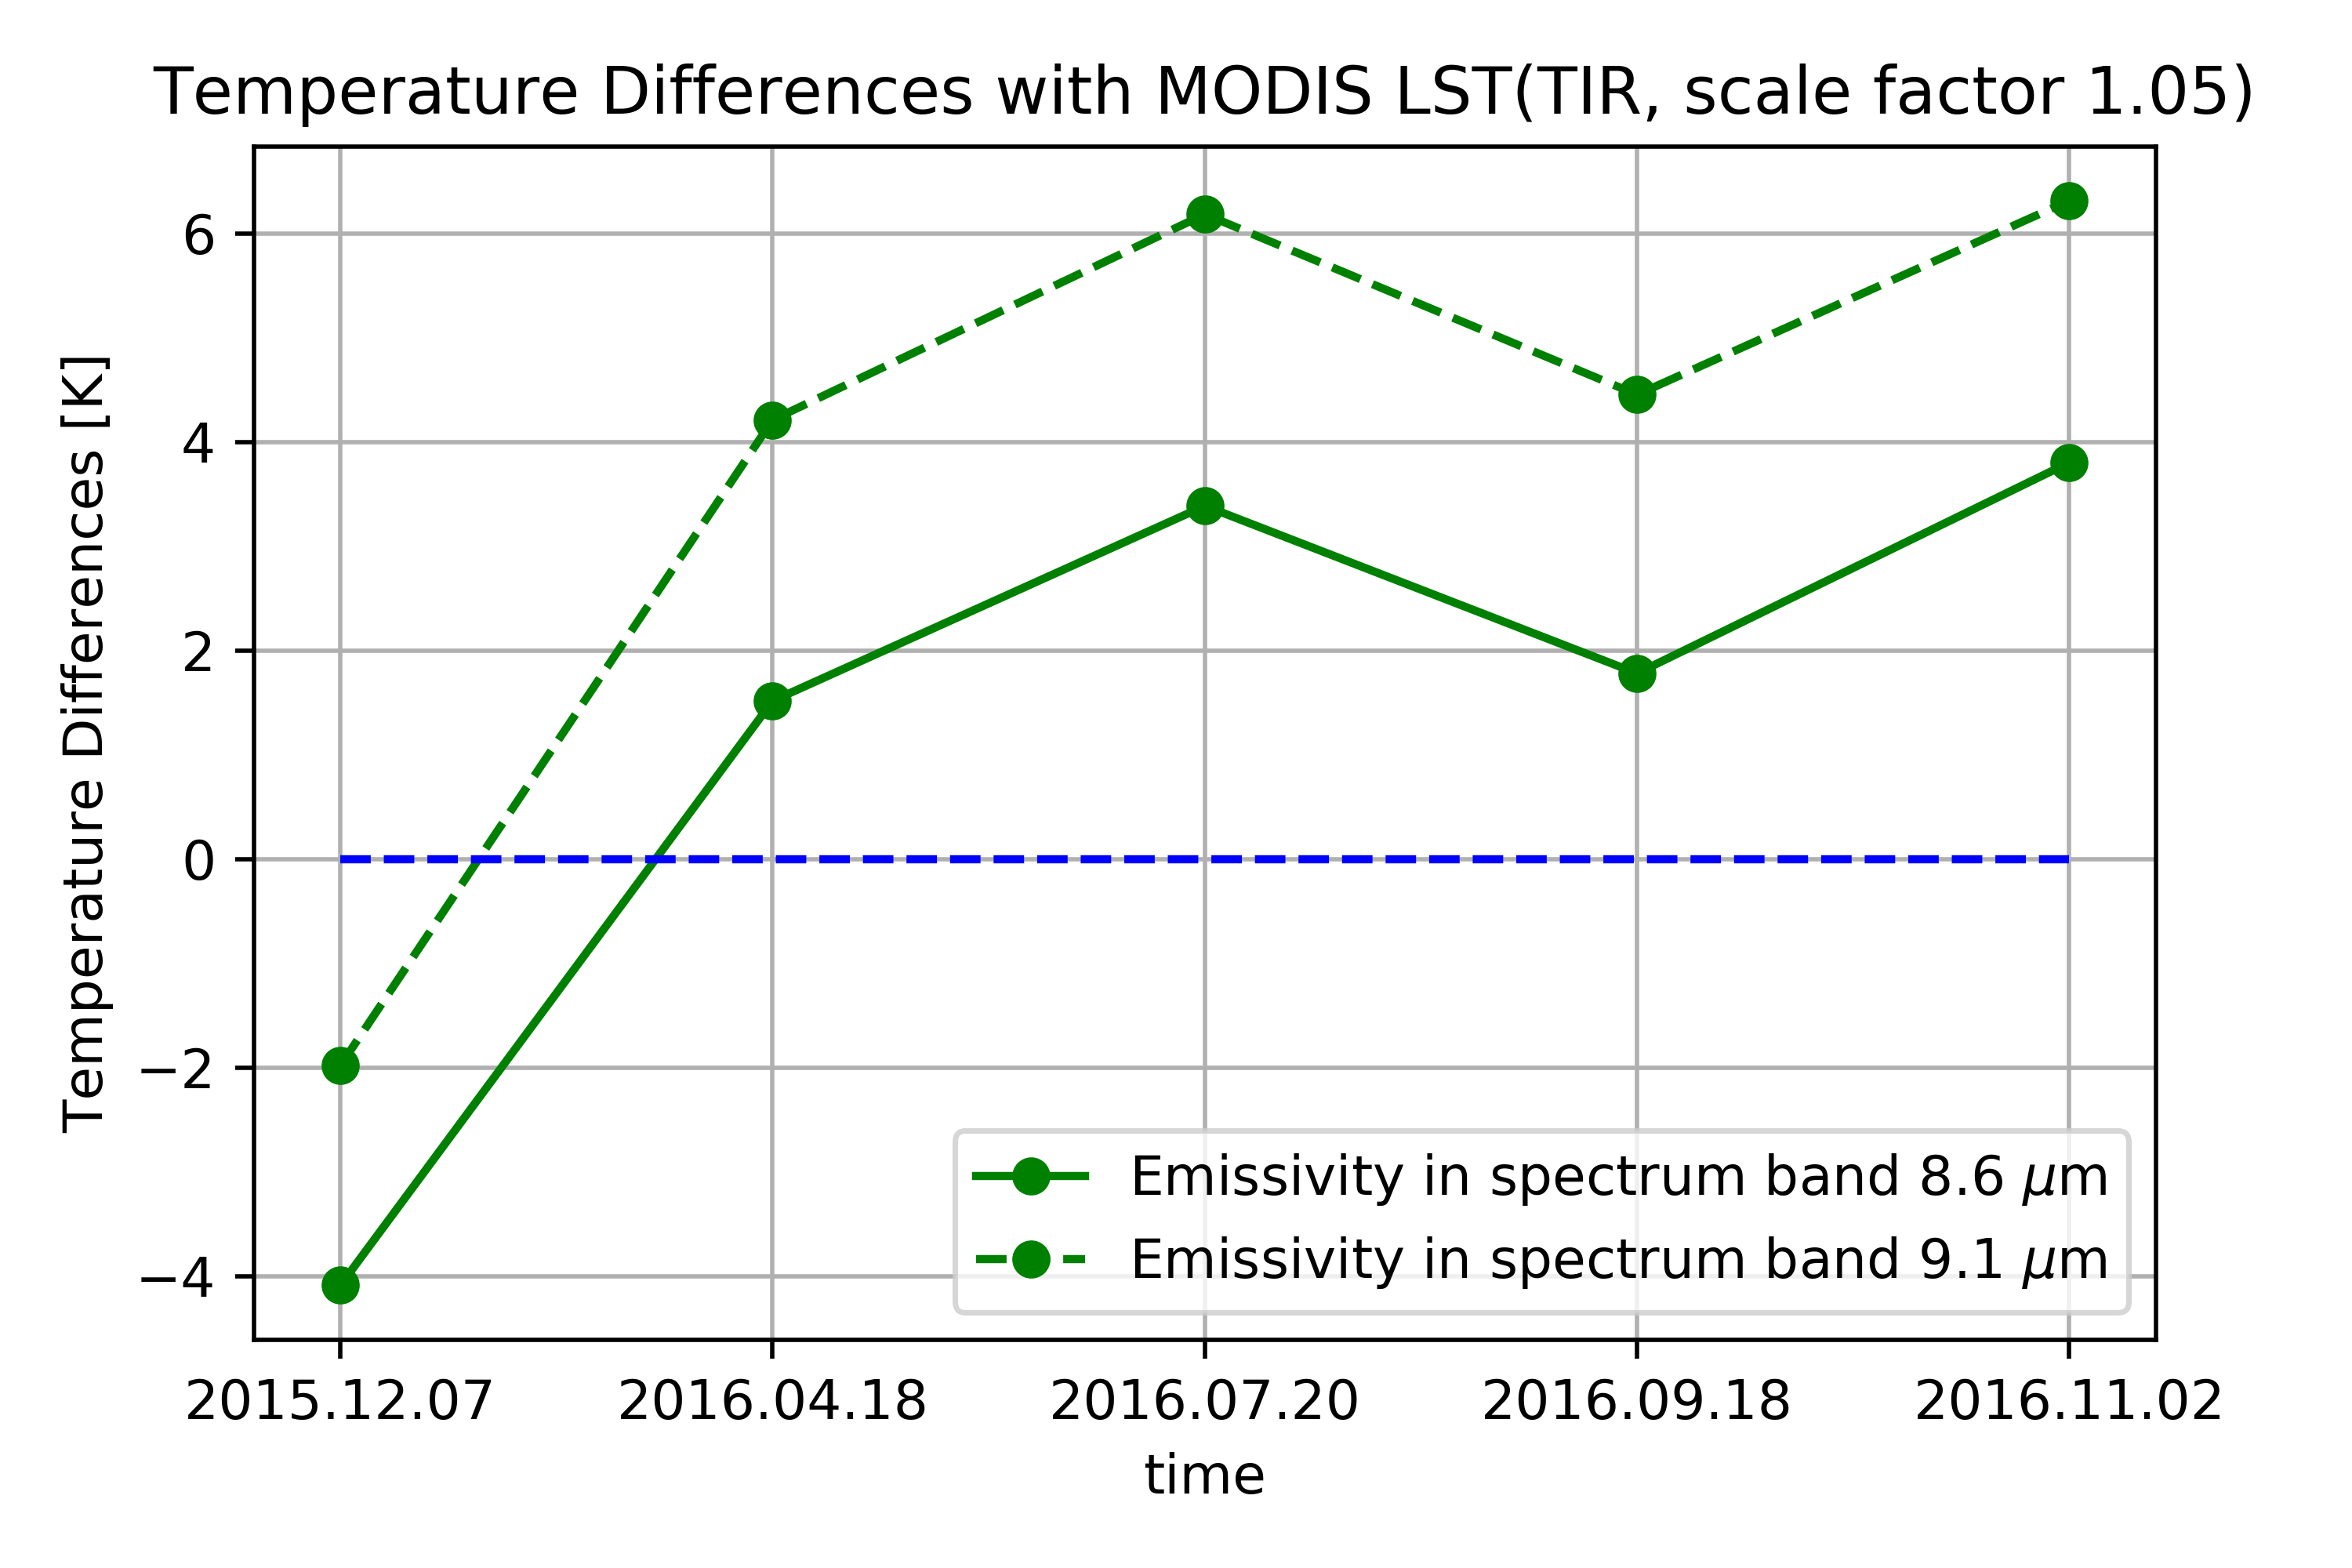
\includegraphics[width = 0.8\linewidth]{diff_emi_tir2.png}}
\caption{Temperature differences (Lybia-1) between the surface temperature maps from MITIP with certain scale factor and MODIS LST.}
\label{fig:diff_emi_Lybia2}
\end{figure}

\noindent After choosing an appropriate emissivity map, similar comparisons between TET-1 surface temperature maps and MODIS LST can be carried out. As what has been done in previous section, several sub-areas are selected distributed over the Libya-1 scenes and the mean temperature difference over all the sub-areas are used to do the comparisons as well.\\

\begin{figure}[!htbp]
\centering
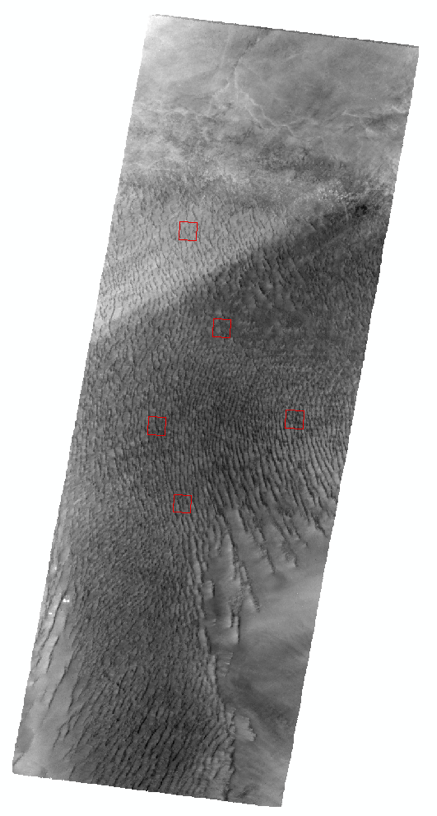
\includegraphics[width = 0.5\textwidth]{Libya-1.png}
\caption{The example figure of Libya-1. The red rectangles represent the selected sub-areas.}
\label{fig:Libya1_sub_areas}
\end{figure}

\begin{figure}[!htbp]
\centering
\subfigure[MIR band]{
\label{fig:Libya-1_sc_mir}
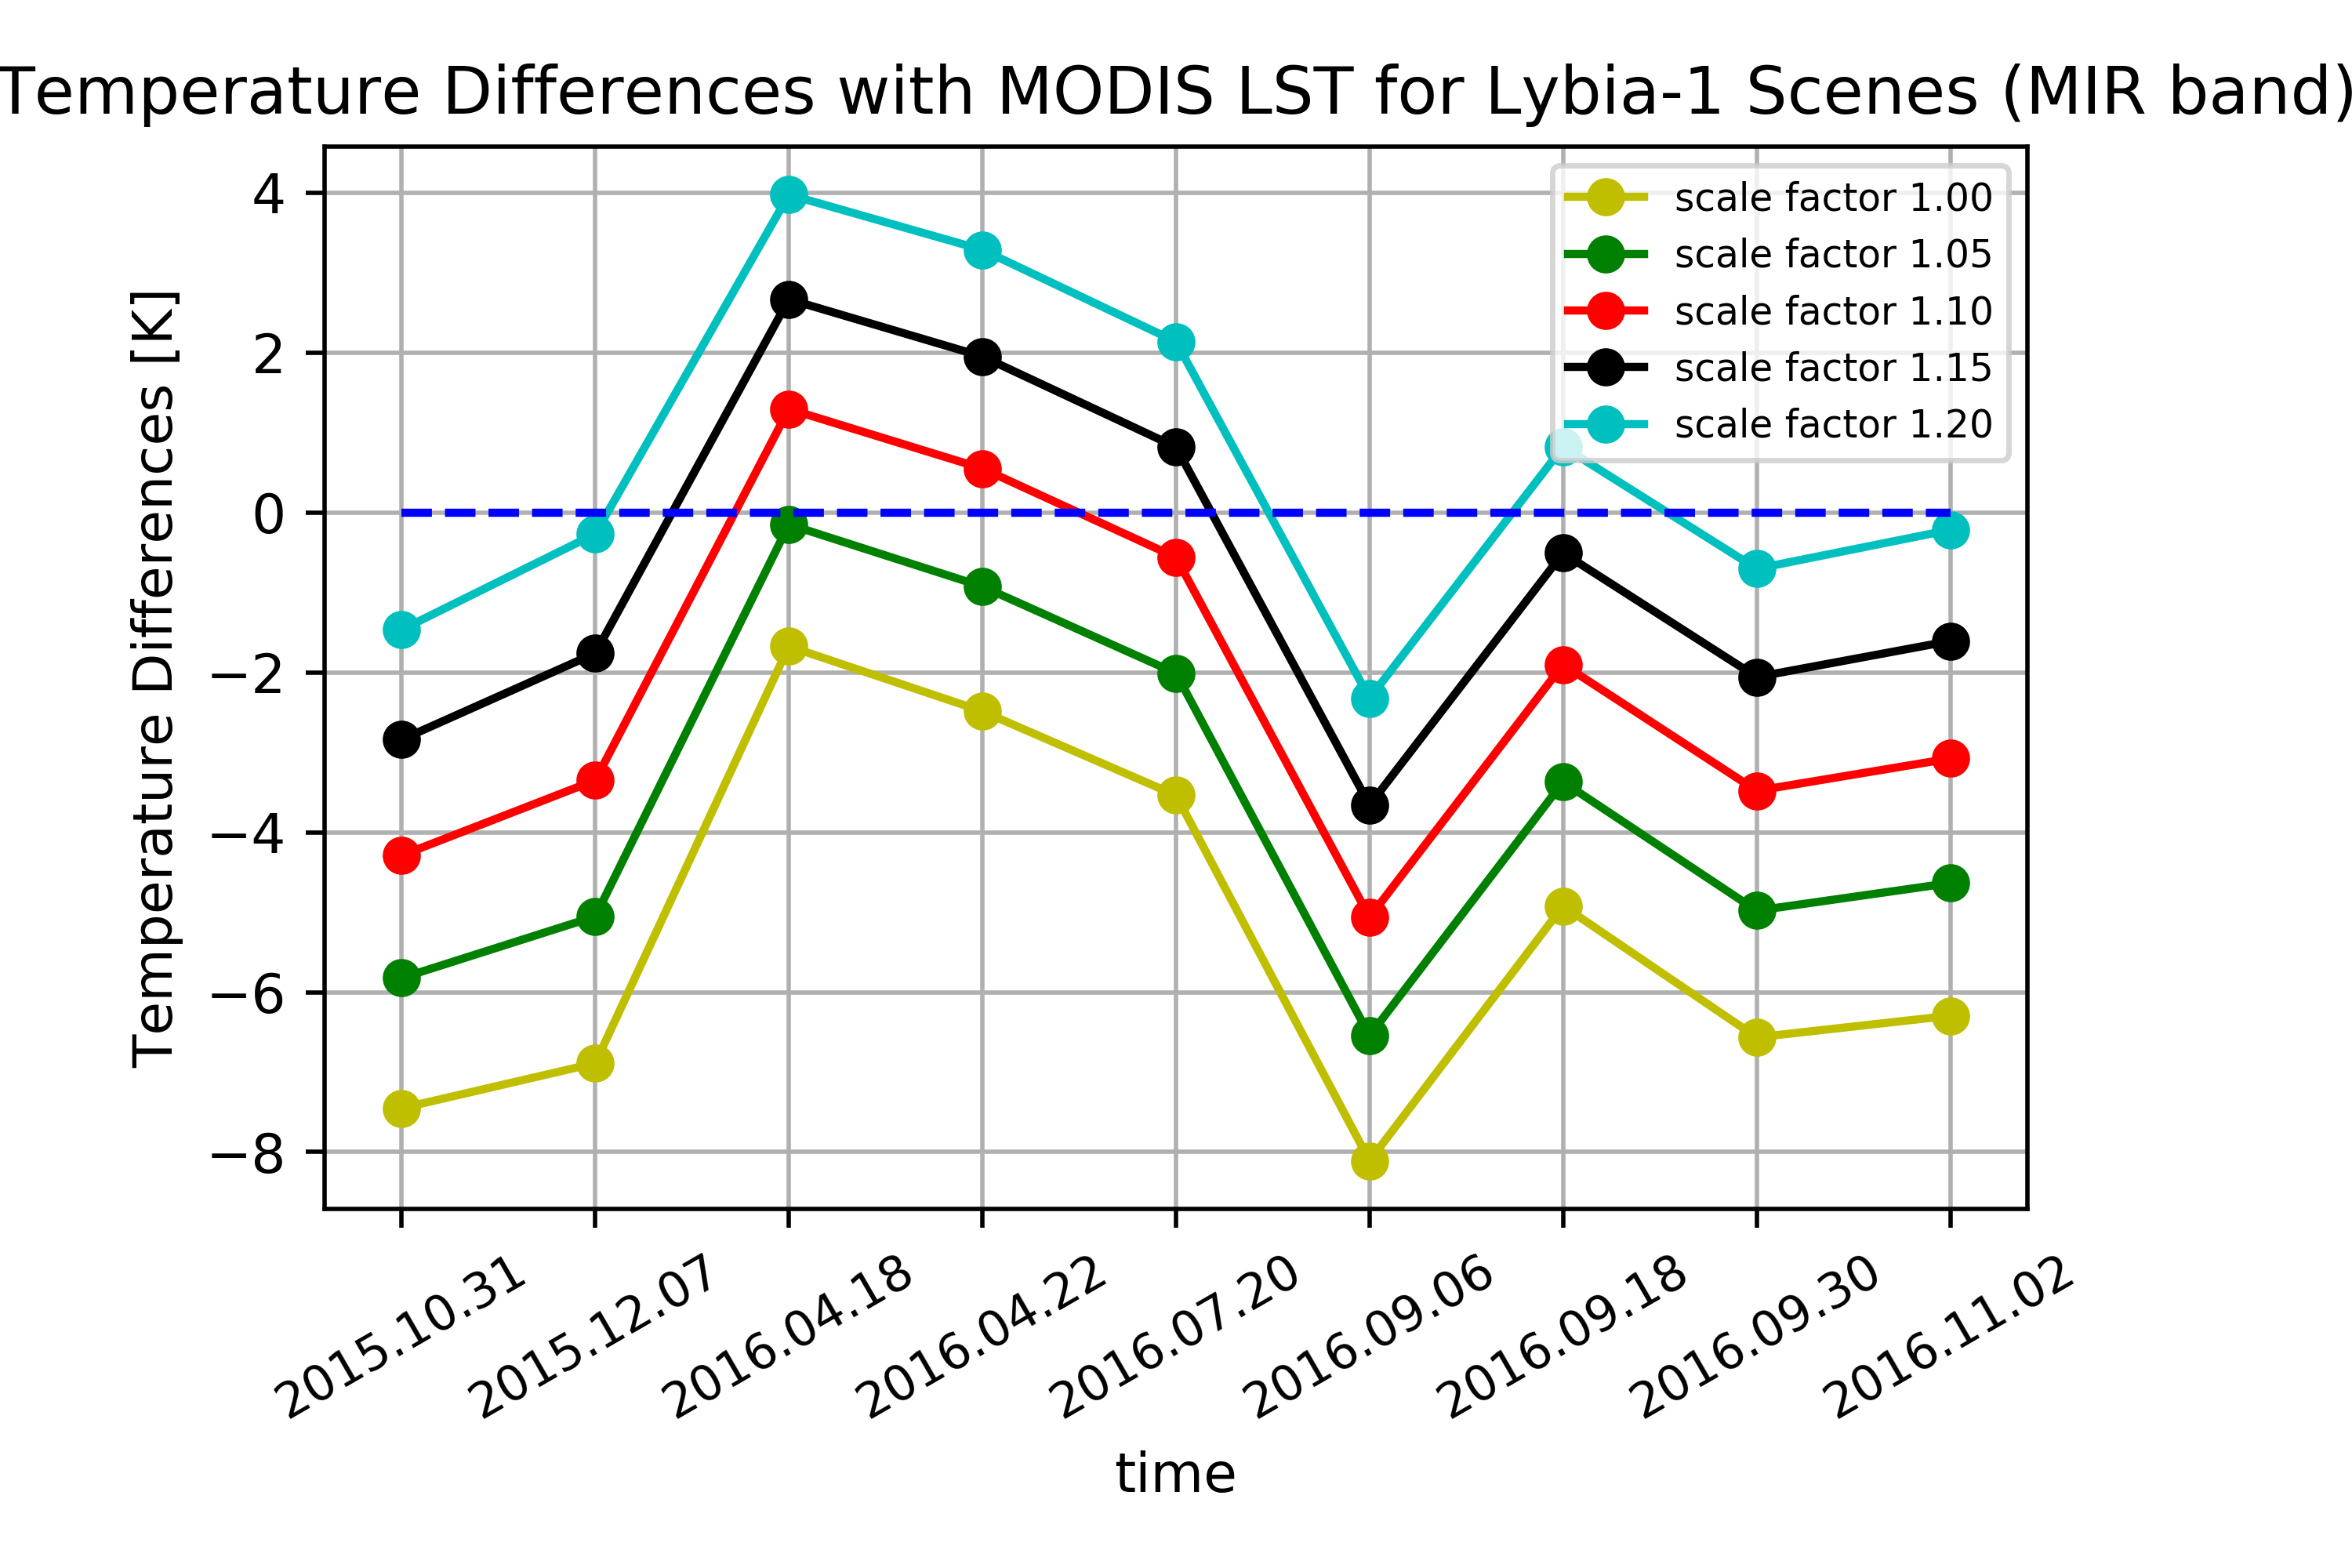
\includegraphics[width = 0.8\linewidth]{Lybia-1_scf_mir.png}}
\hspace{0.5in}
\subfigure[TIR band]{
\label{fig:Libya-1_sc_tir}
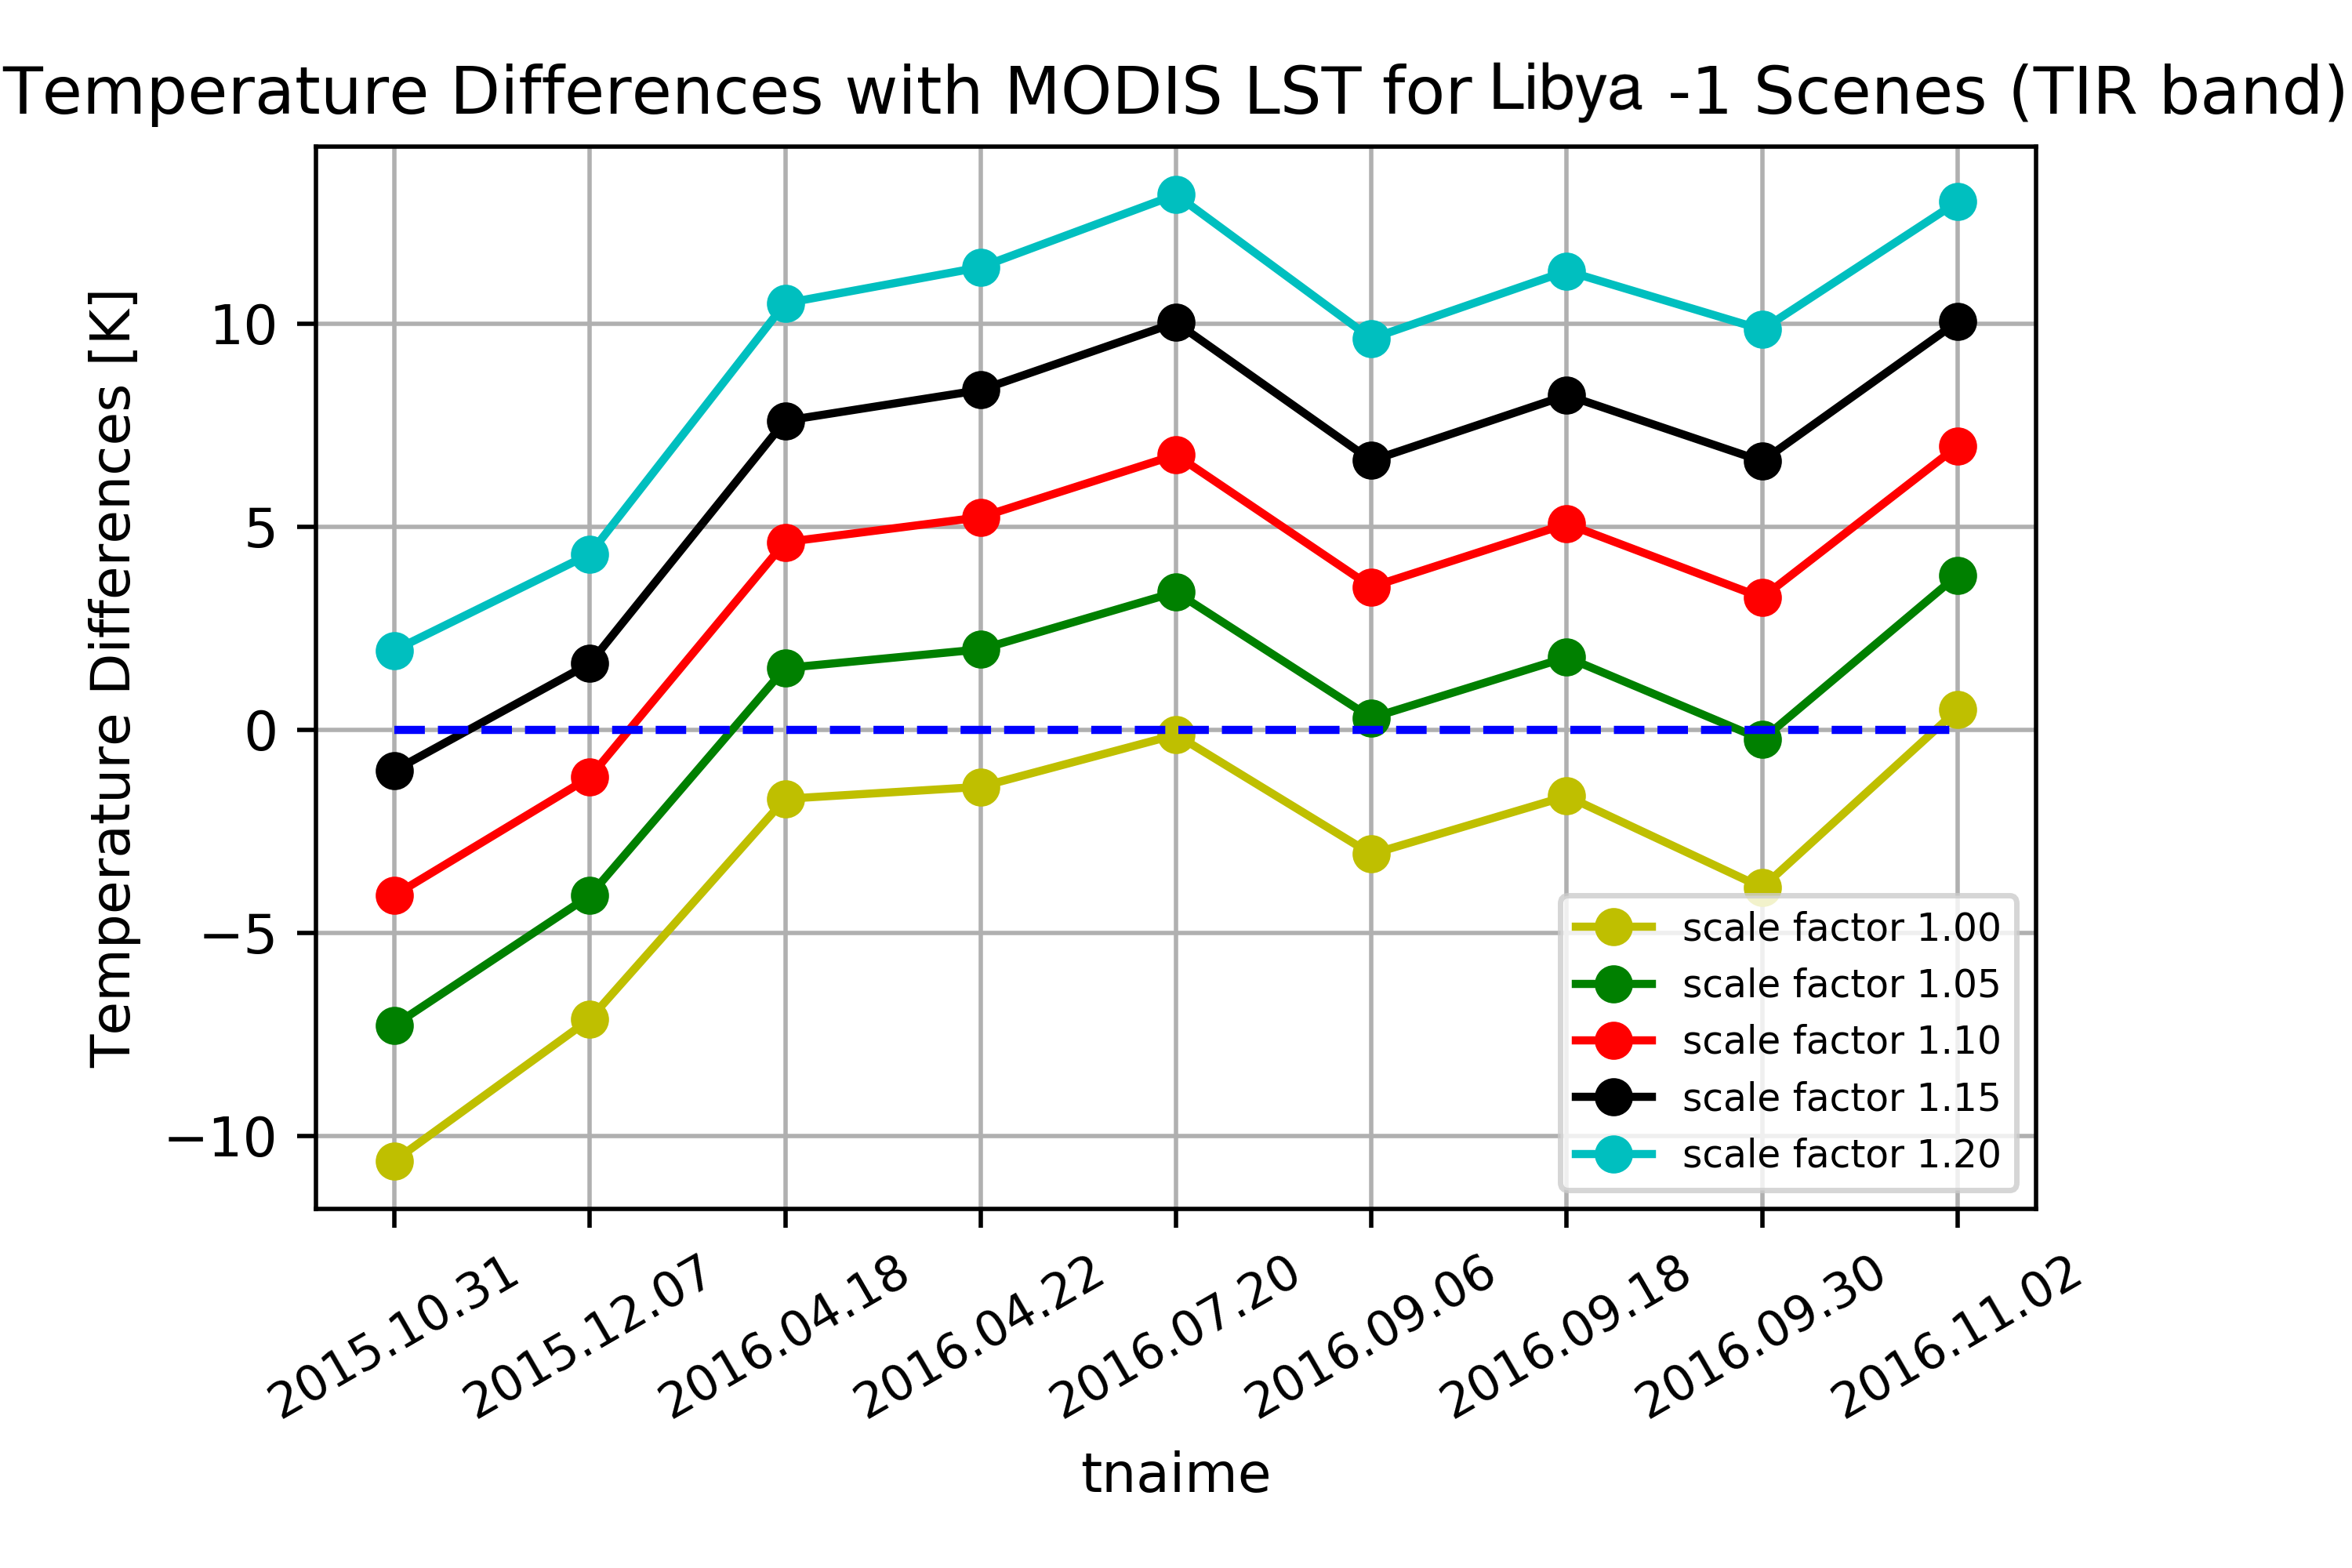
\includegraphics[width = 0.8\linewidth]{Lybia-1_scf_test_tir.png}}
\caption{Tempereature differences between TET-1 surface temperature maps and MODIS LST (Libya-1).}
\label{fig:Libya-1_sc_mir_tir}
\end{figure}

\noindent As Figure \ref{fig:Libya-1_sc_mir_tir} shows, the temperature differences between MODIS LST and TET-1 surface temperature maps with different scale factors act randomly as well. For the TIR band imageries, again, the scale factor 1.05 achieves the best performances, which can also be seen in Figure \ref{fig:Libya-1_bsc_tir}. For the MIR band imageries, it is clear from the Figure \ref{fig:Libya-1_sc_mir} and Figure \ref{fig:Libya-1_bsc_mir}, much more MIR band imageries require a higher scale factor compared with the situation of doing comparison with the MODIS SST. This is also why the scale factor 1.15 is selected as the optimal scale factor for the MIR band imageries. On one hand, it can achieve a good results for these scenes require a higher scale factor. On the other hand, it will not over calibrate these scenes require a lower scale factor. All in all, the scale factor 1.15 for the MIR band imageries perform best over all scenes of different times.\\

\begin{figure}[!htbp]
\centering
\subfigure[MIR band]{
\label{fig:Libya-1_bsc_mir}
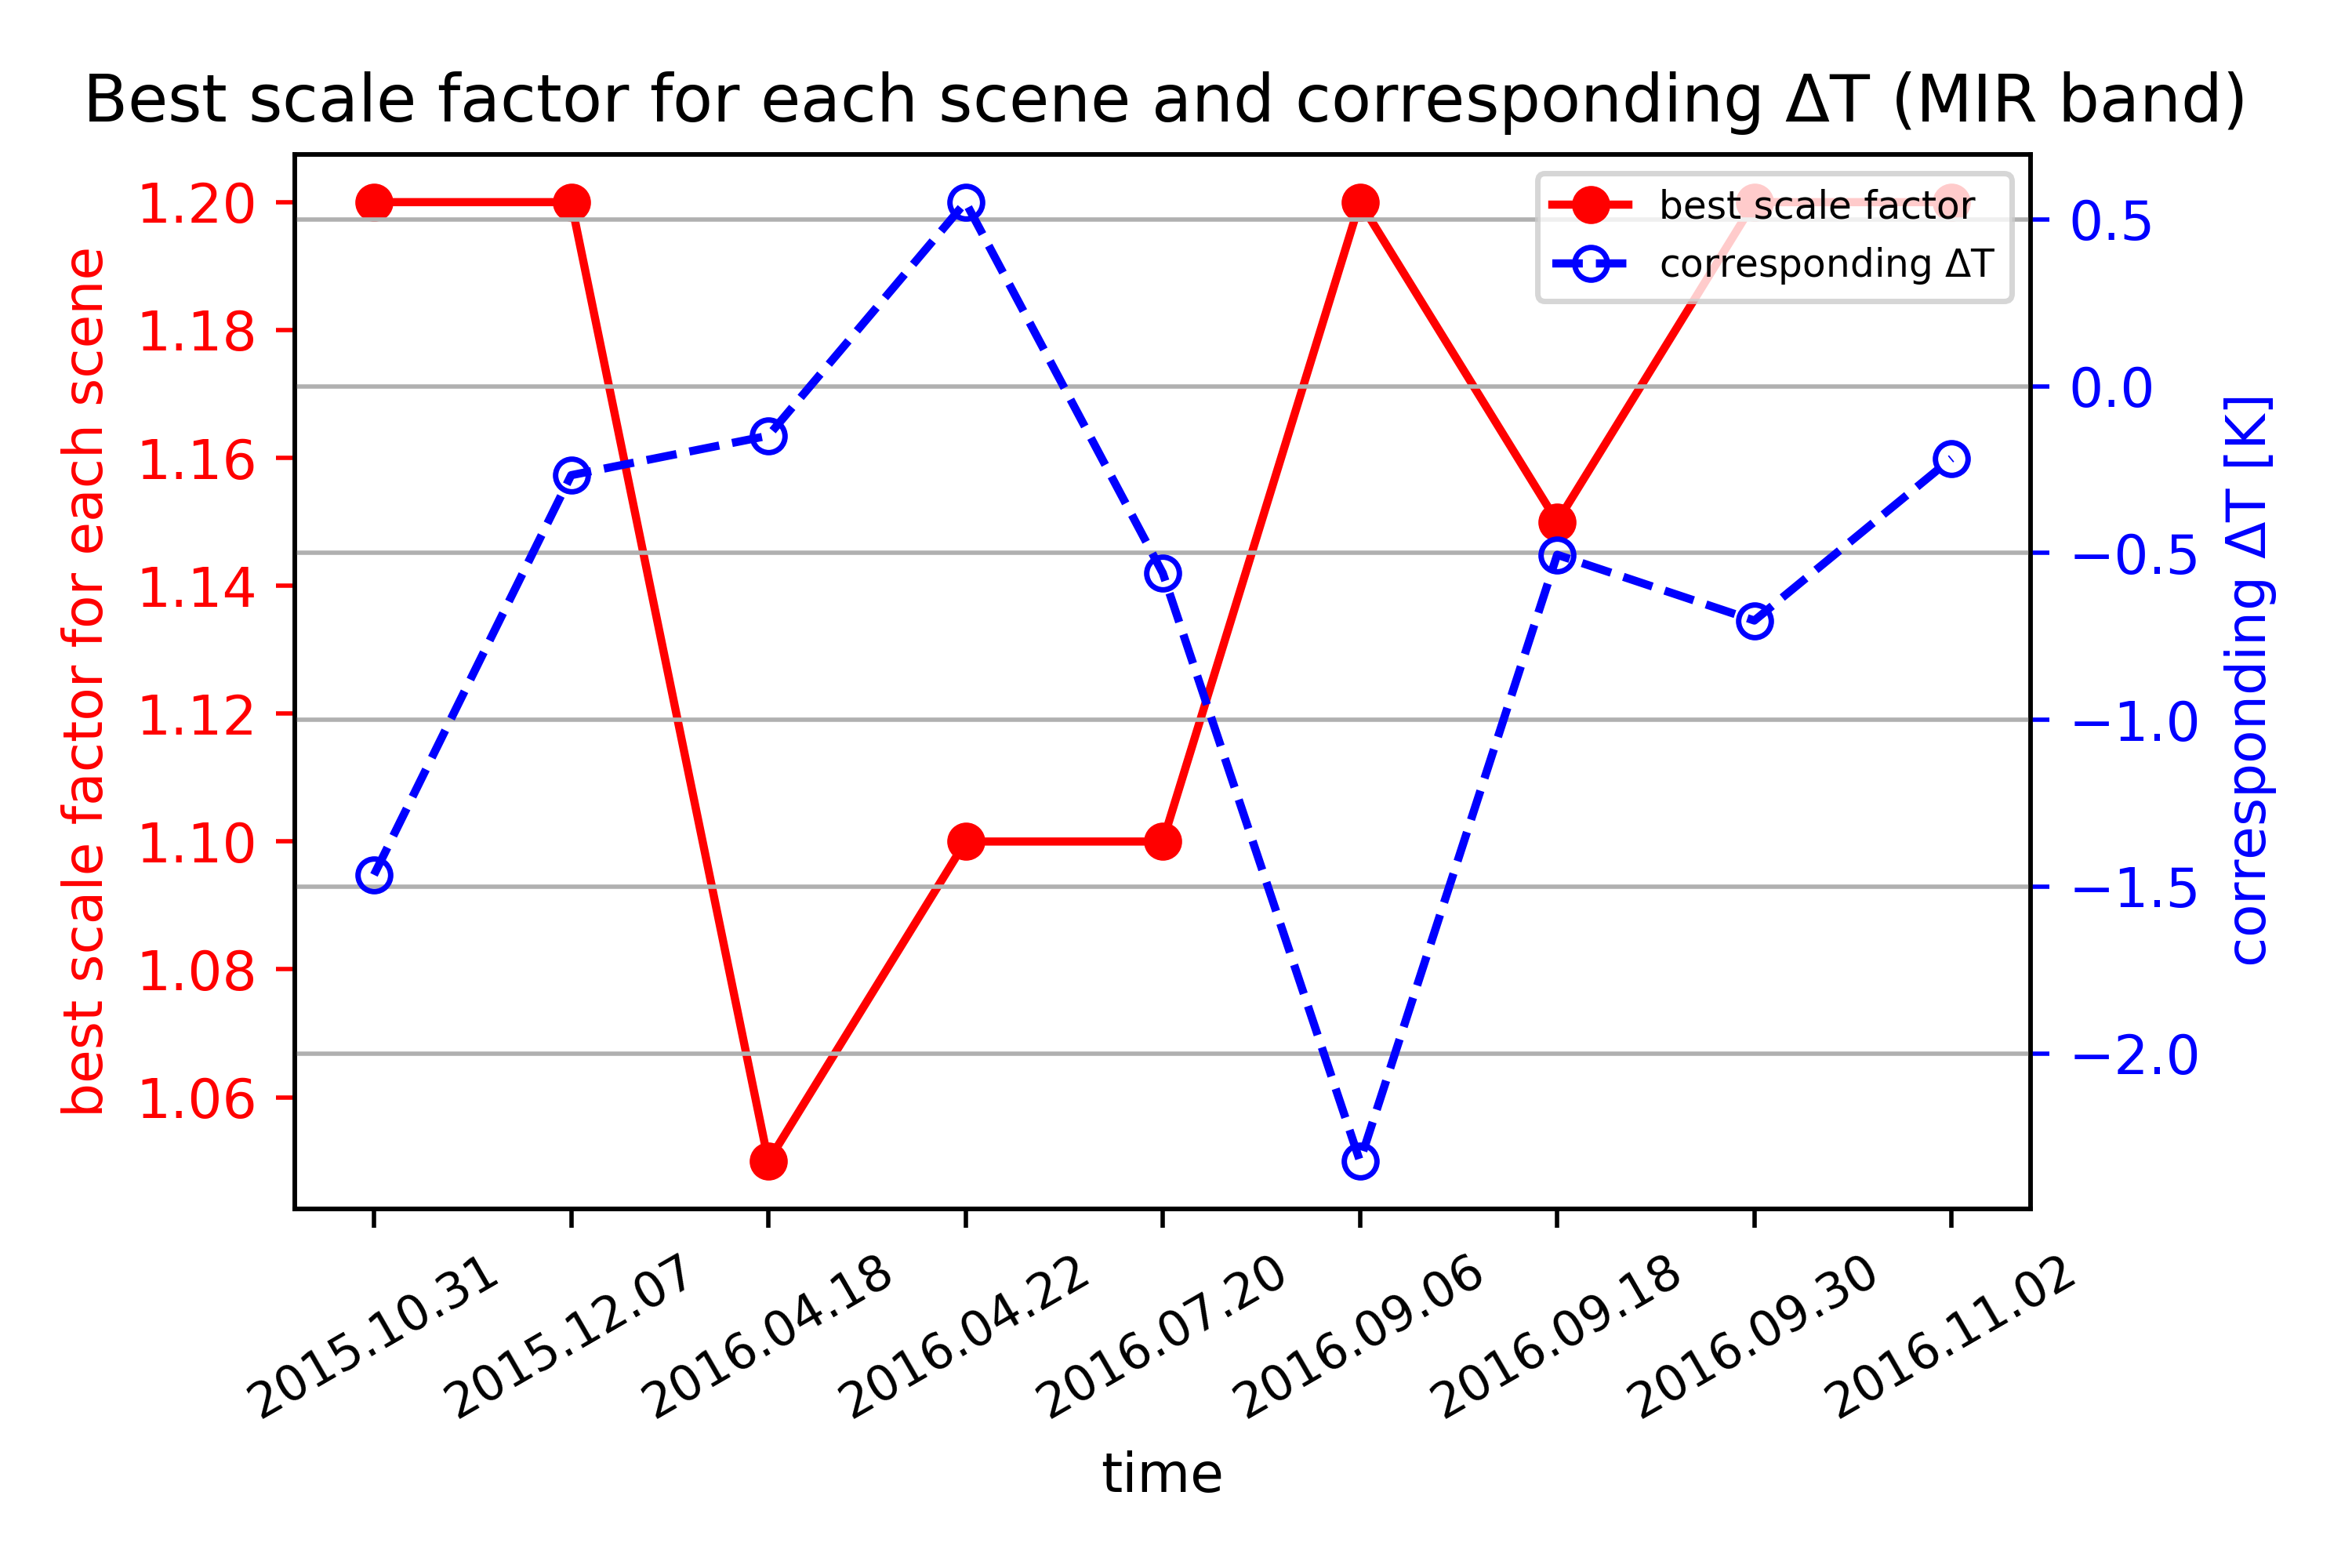
\includegraphics[width = 0.8\linewidth]{Lybia-1_bsc&tem_mir.png}}
\hspace{0.5in}
\subfigure[TIR band]{
\label{fig:Libya-1_bsc_tir}
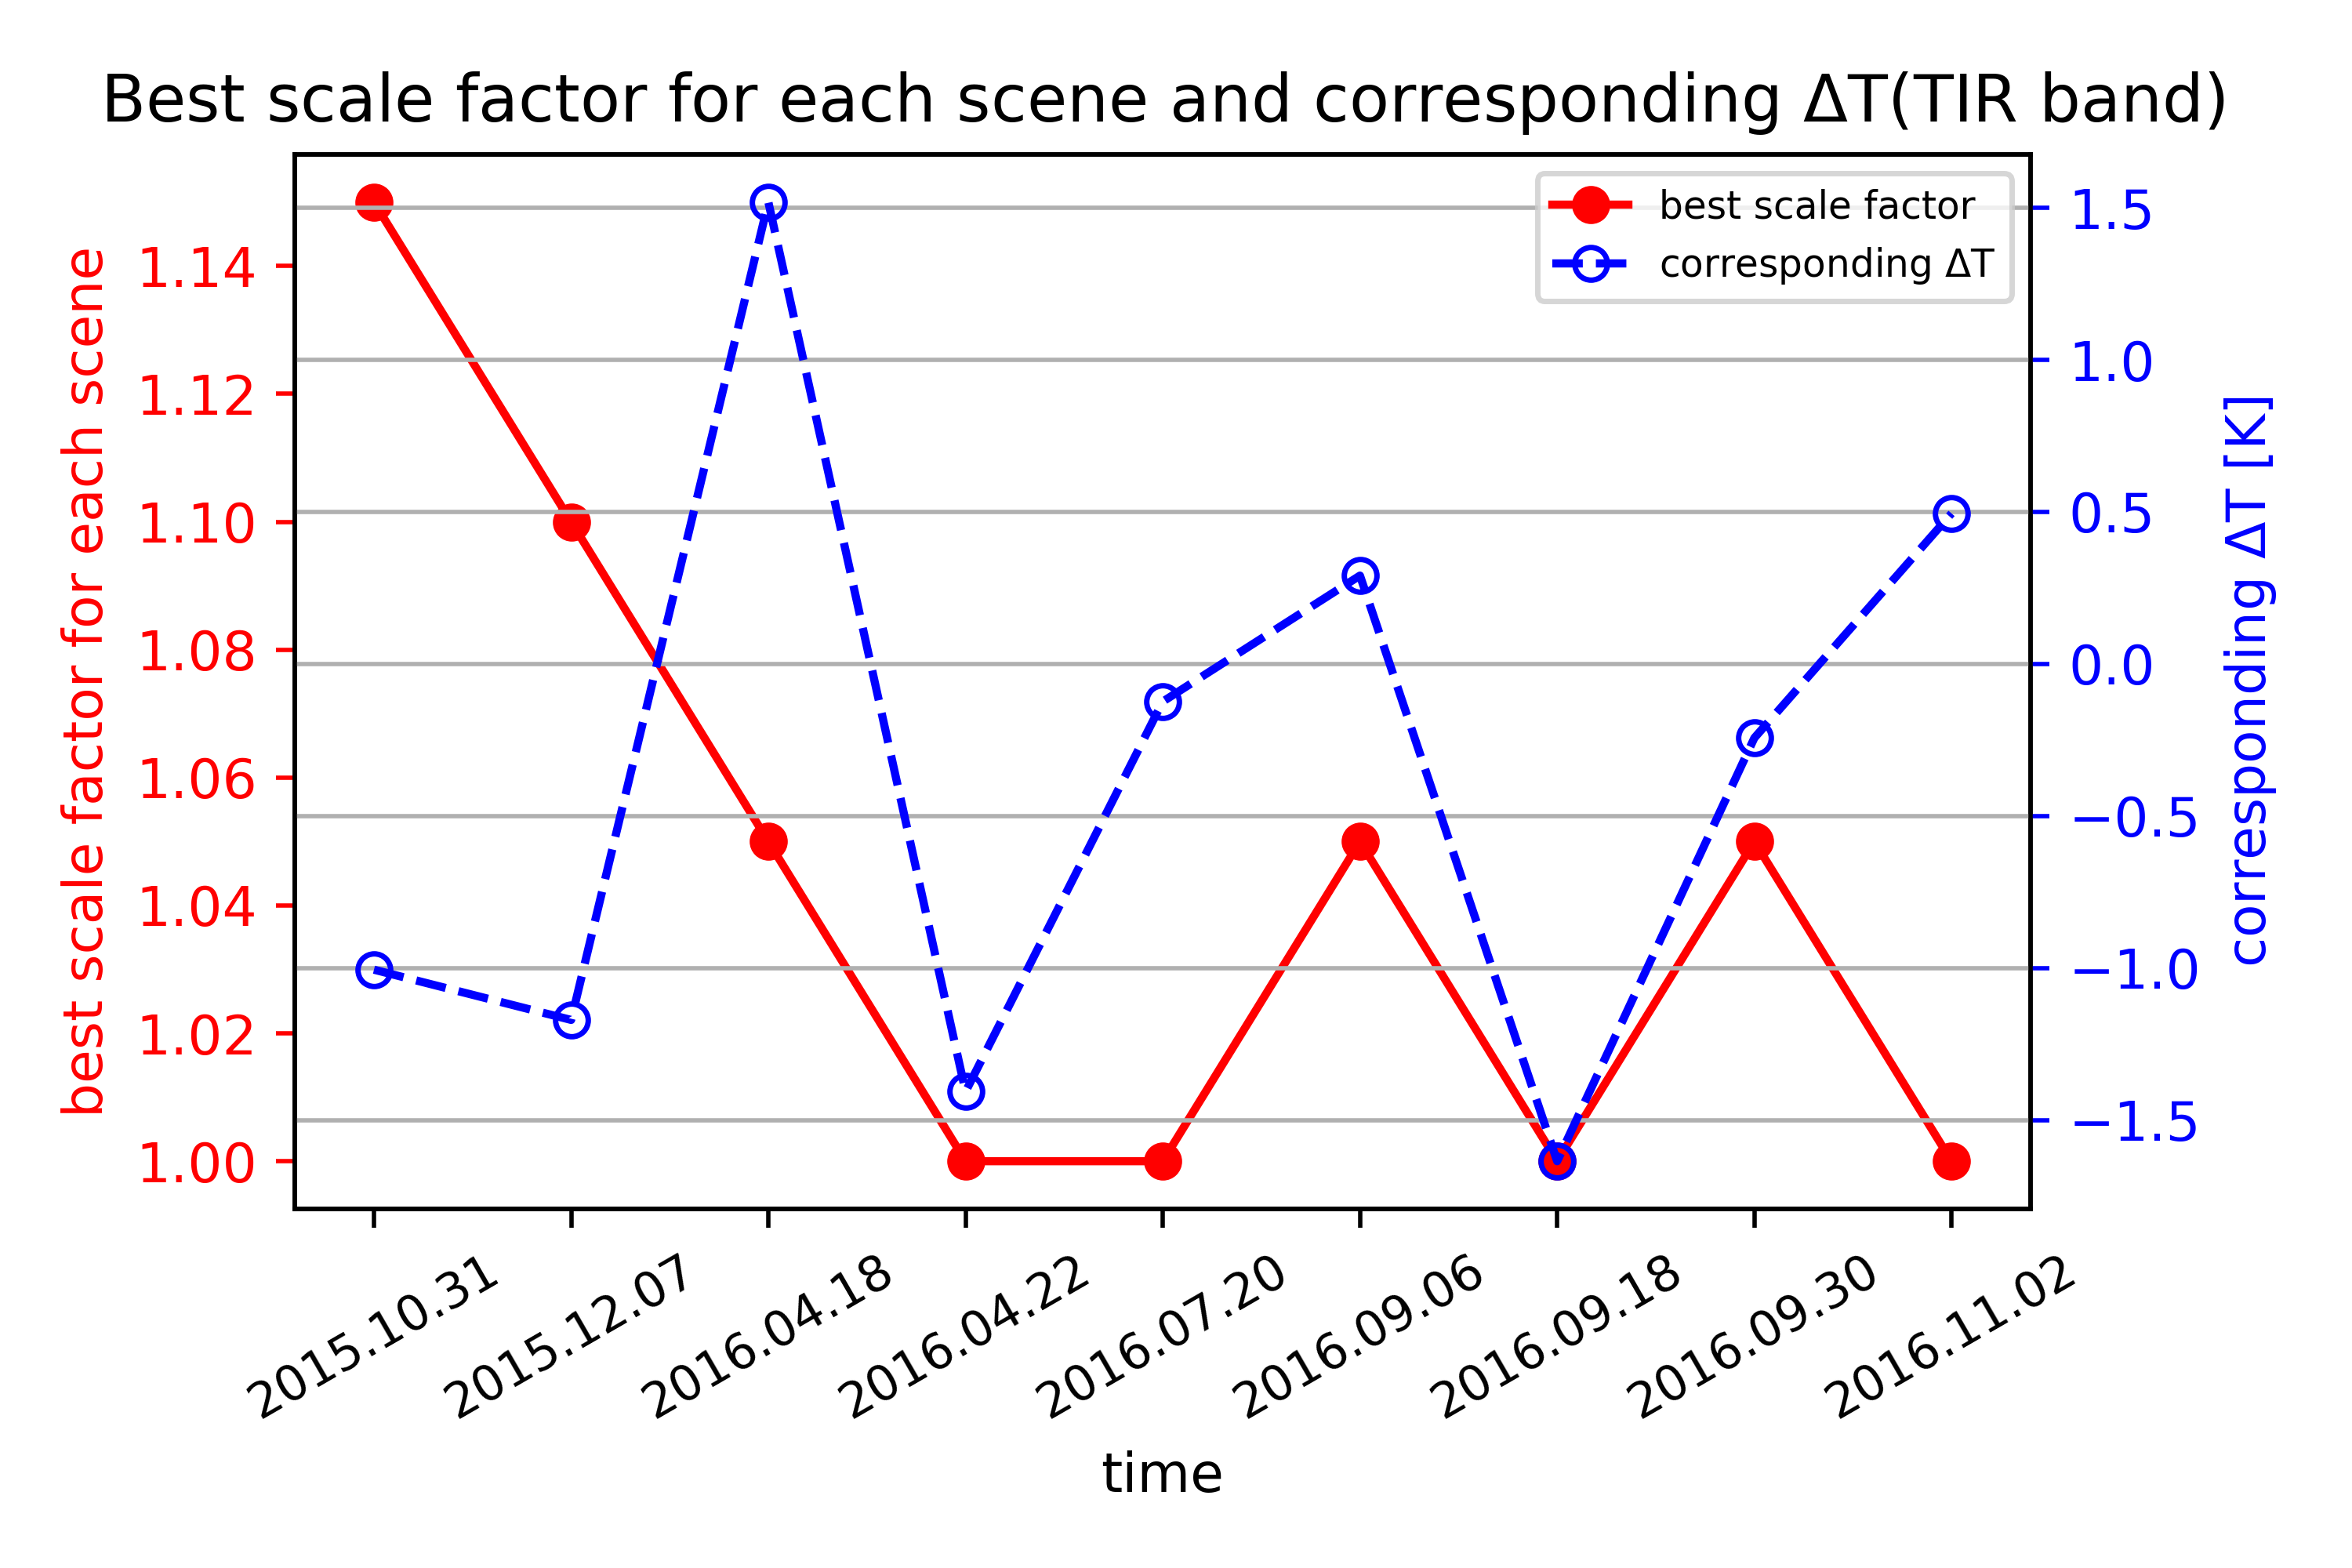
\includegraphics[width = 0.8\linewidth]{Lybia-1_bsc&tem_tir.png}}
\caption{The best scale factors for each Lybia-1 scenes and its corresponding temperature differences. The red solid line is the best scale factor for each Libya-1 scene. The blue dashed line is the minimal temperature differences resulted from that scale factor.}
\label{fig:Libya-1_bsc_mir_tir}
\end{figure}

\begin{figure}[!htbp]
\centering
\subfigure[MIR band]{
\label{fig:Lybia-1_bsc&temCom_mir}
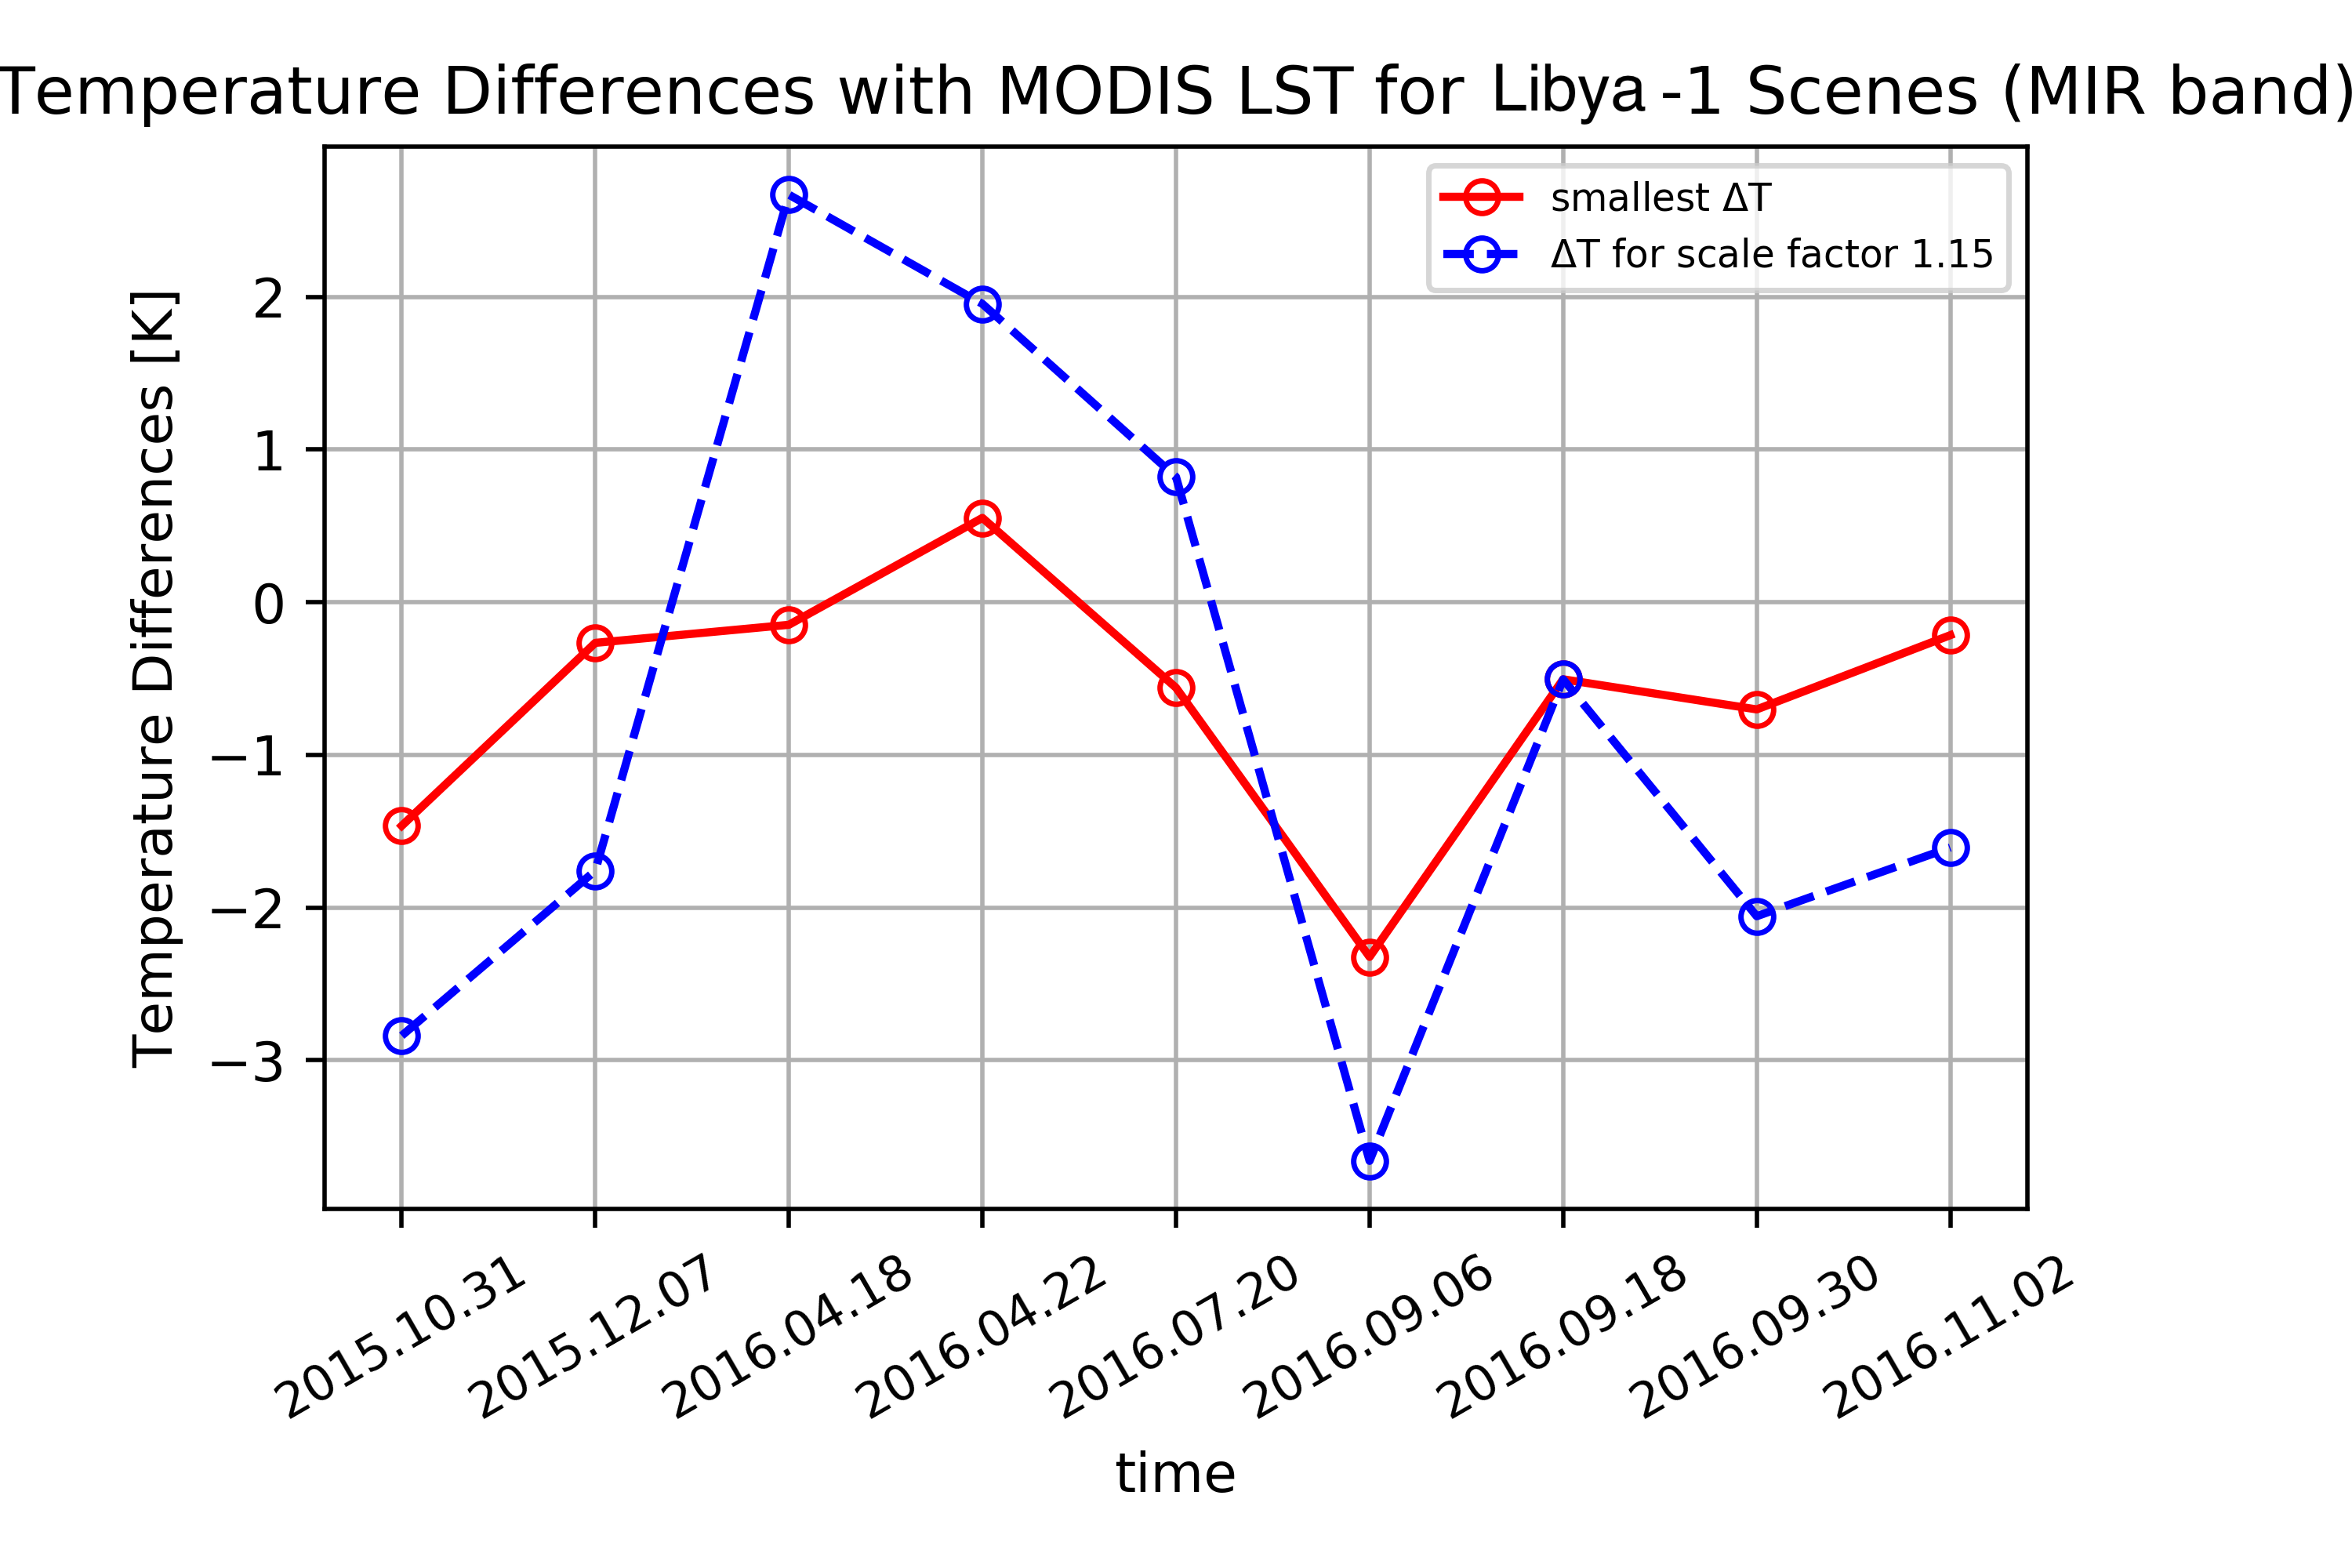
\includegraphics[width = 0.8\linewidth]{Lybia-1_bsc&temCom_mir.png}}
\hspace{0.5in}
\subfigure[TIR band]{
\label{fig:Lybia-1_bsc&temCom_tir}
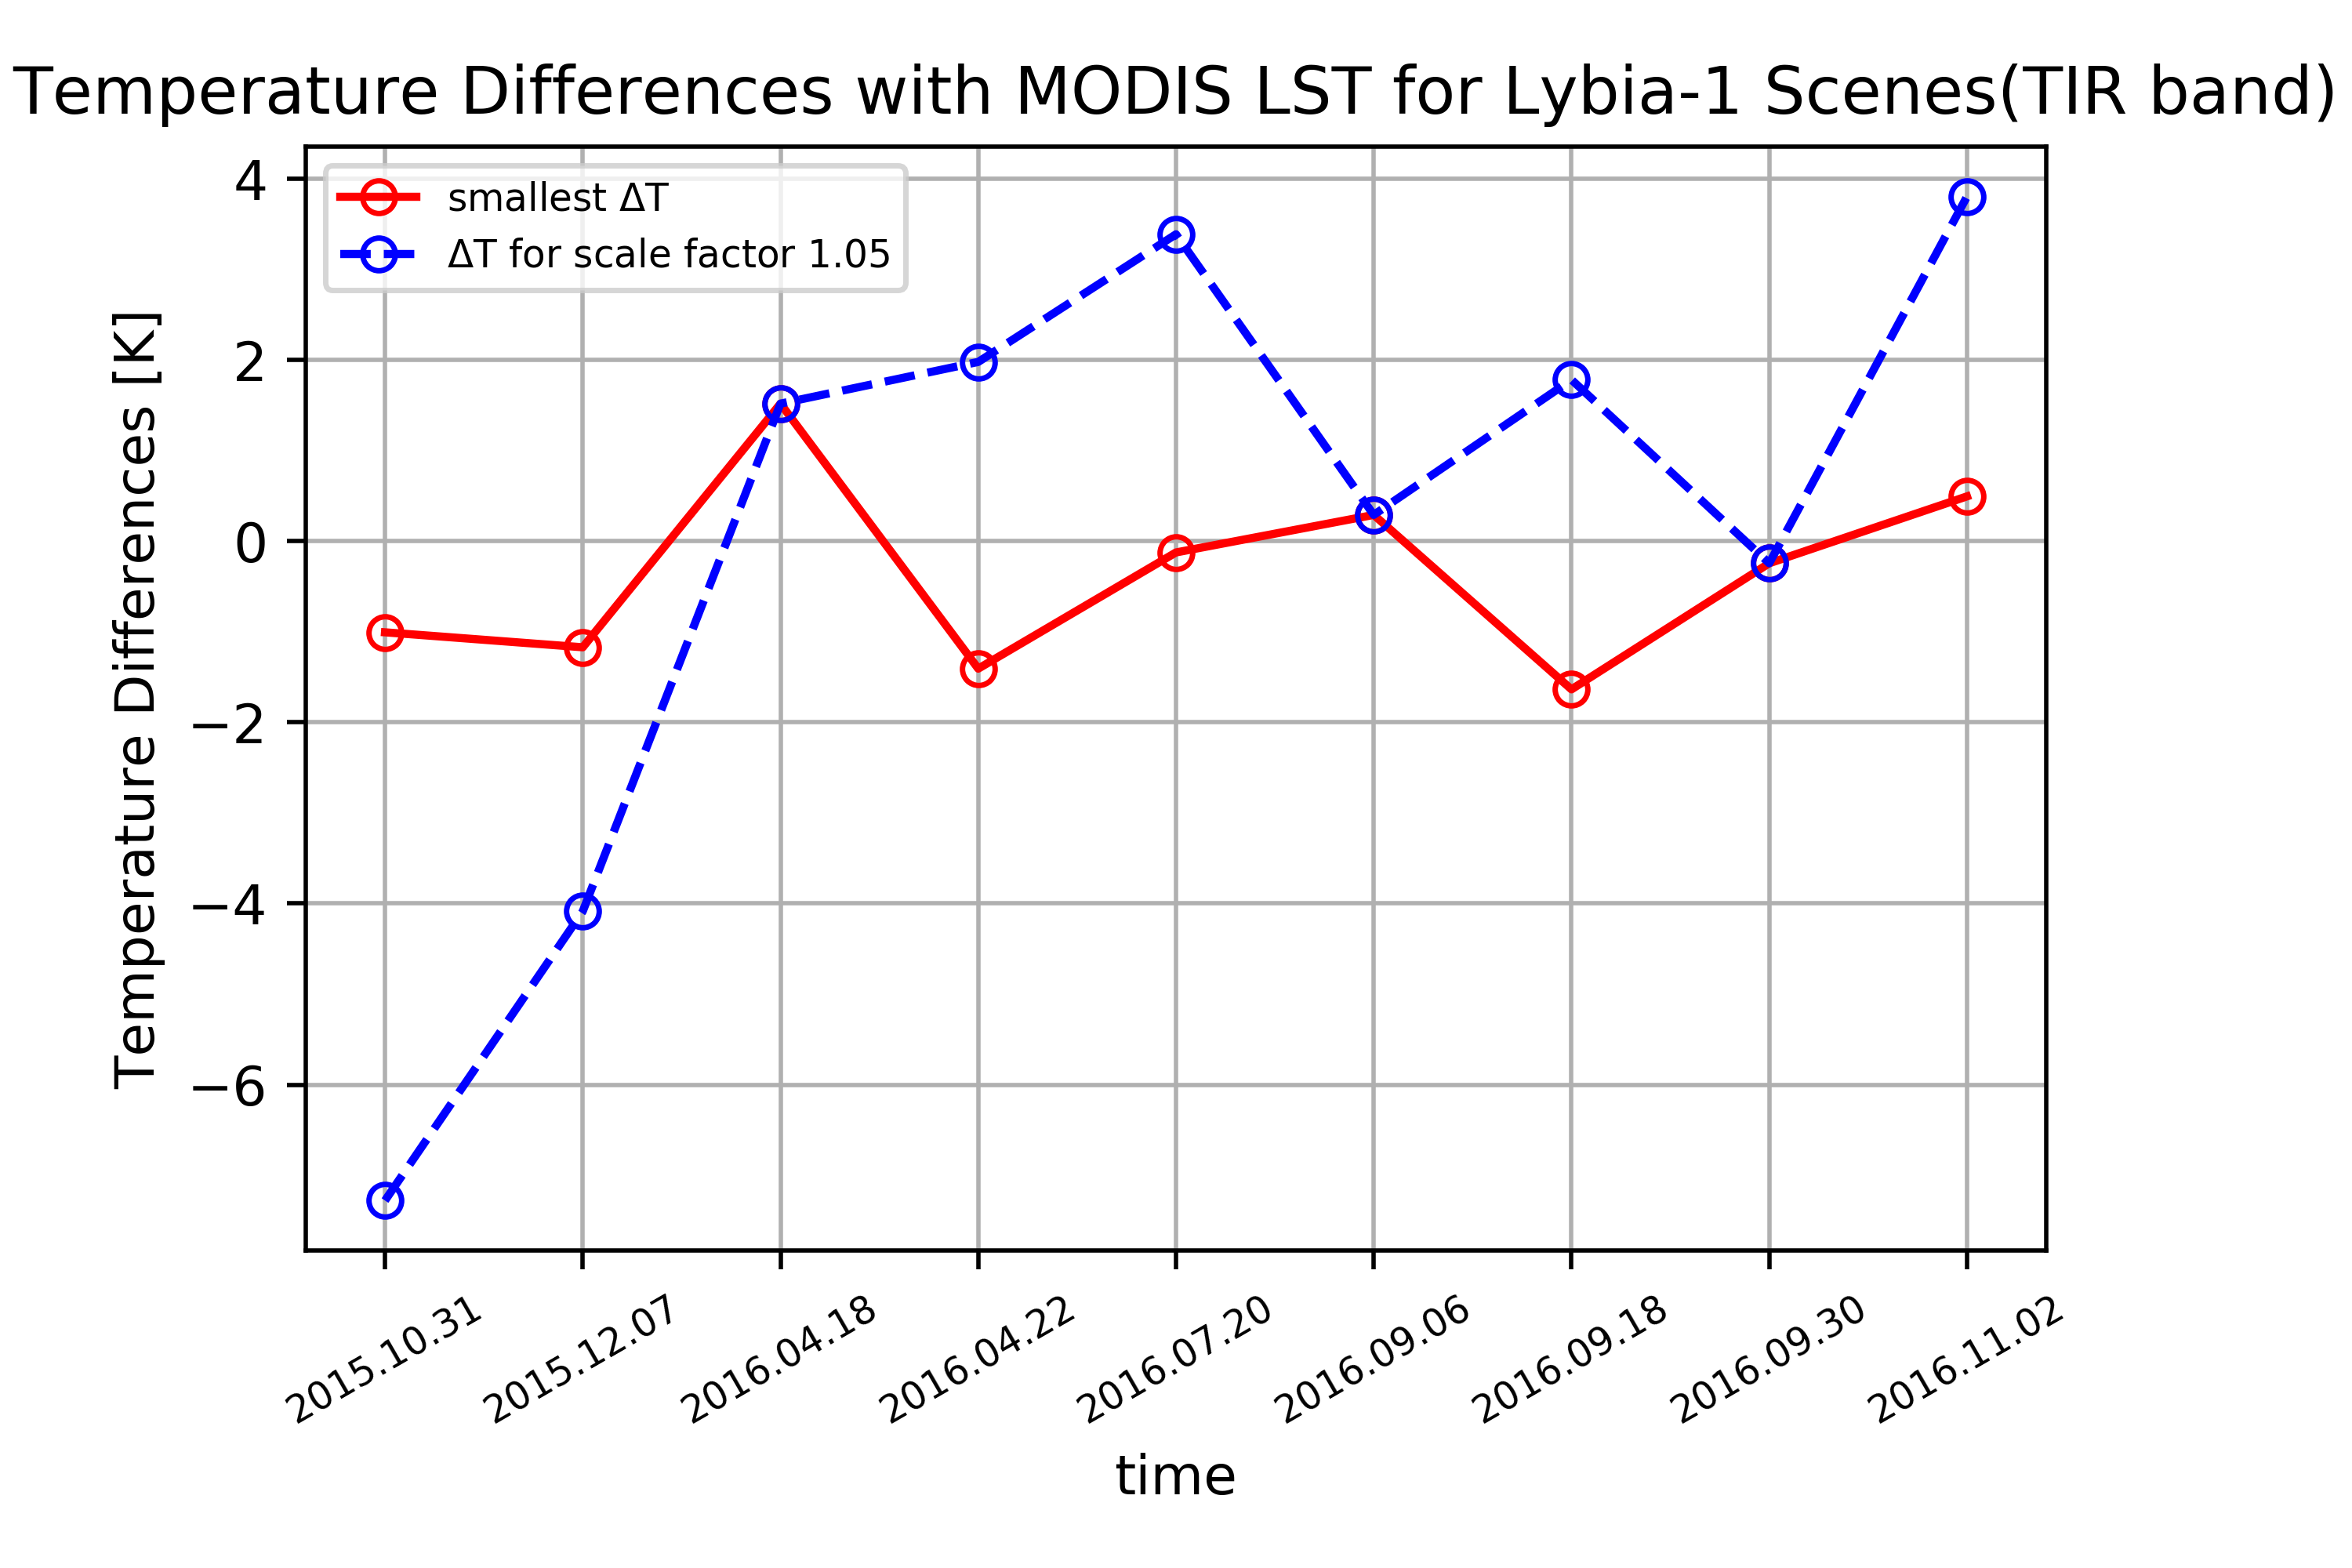
\includegraphics[width = 0.8\linewidth]{Lybia-1_bsc&temCom_tir.png}}
\caption{The minimal temperature differences and the temperature differences resulted from scale factor 1.15 and scale factor 1.05. The red solid line is the minimal temperature differences for each Etna scene. The blue dashed line is the temperature differences resulted from the selected scale factors for MIR and TIR band imageries, scale factor 1.15 (upper) and scale factor 1.05 (lower), respectively.}
\label{fig:Lybia-1_bsc&temCom}
\end{figure}

\noindent As Figure \ref{fig:Lybia-1_bsc&temCom} shows, for the TET-1 MIR and TIR band imageries of the site Libya-1, the scale factor 1.15 and 1.05 are not the optimal scale factors for every scene. But the temperature differences they made are very close to the minimal temperature differences. What's more, the choices enable us to ignore the difference between water-dominated or land-dominated scenes because the optimal scale factors for the Libya-1 scenes are the same as the optimal scale factors for the Etna scenes. Of course, latter, the transferability of the scale factors selected from the Libya-1 scenes will be tested.\\

%-----------------------------------
%	SUBSECTION 5
%-----------------------------------

\subsection{transferability test (LST)}
After the selection of the optimal scale factors, as what has been done after the comparisons with the MODIS SST, the transferability of  the chosen scale factors will be tested using several scenes of other sites. Here, scenes of Libya-2 are used as test scenes. Figure \ref{fig:Libya2_sub_areas} is an example scene of Libya-2.\\

\begin{figure}[!htbp]
\centering
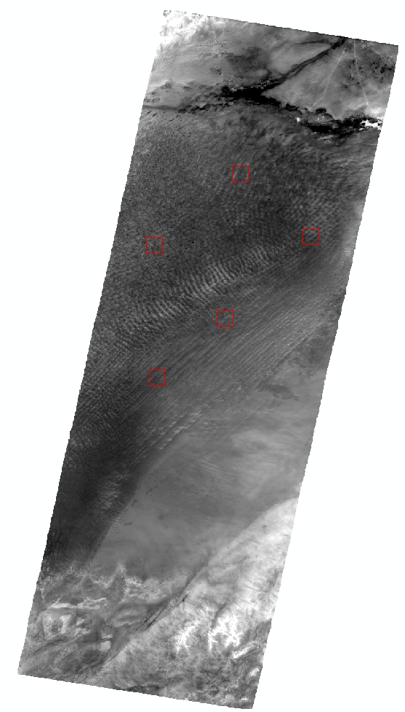
\includegraphics[width = 0.5\textwidth]{Libya-2.png}
\caption{The example figure of Libya-2. The red rectangles represent the selected sub-areas.}
\label{fig:Libya2_sub_areas}
\end{figure}

\noindent Besides the chosen scale factor 1.15 for MIR band imagery and 1.05 for TIR band imagery, the performance of the scale factor 1.10 and 1.20 are also presented for the TET-1 MIR band imagery as comparison and for TIR band imagery, the performances of scale factor 1.00 and 1.10 are displayed as well for the same purpose. The results arde presented in Figure \ref{fig:LST_test}. The situation is similar with the situation of Section 4.1.3. Scale factor 1.15 for MIR band imagery and 1.05 for TIR band imagery are not always optimal scale factors for every scenes, however, they demonstrate better performance than other scale factors over time.\\

\begin{figure}[!htbp]
\centering
\subfigure[MIR band]{
\label{fig:LST_test_mir}
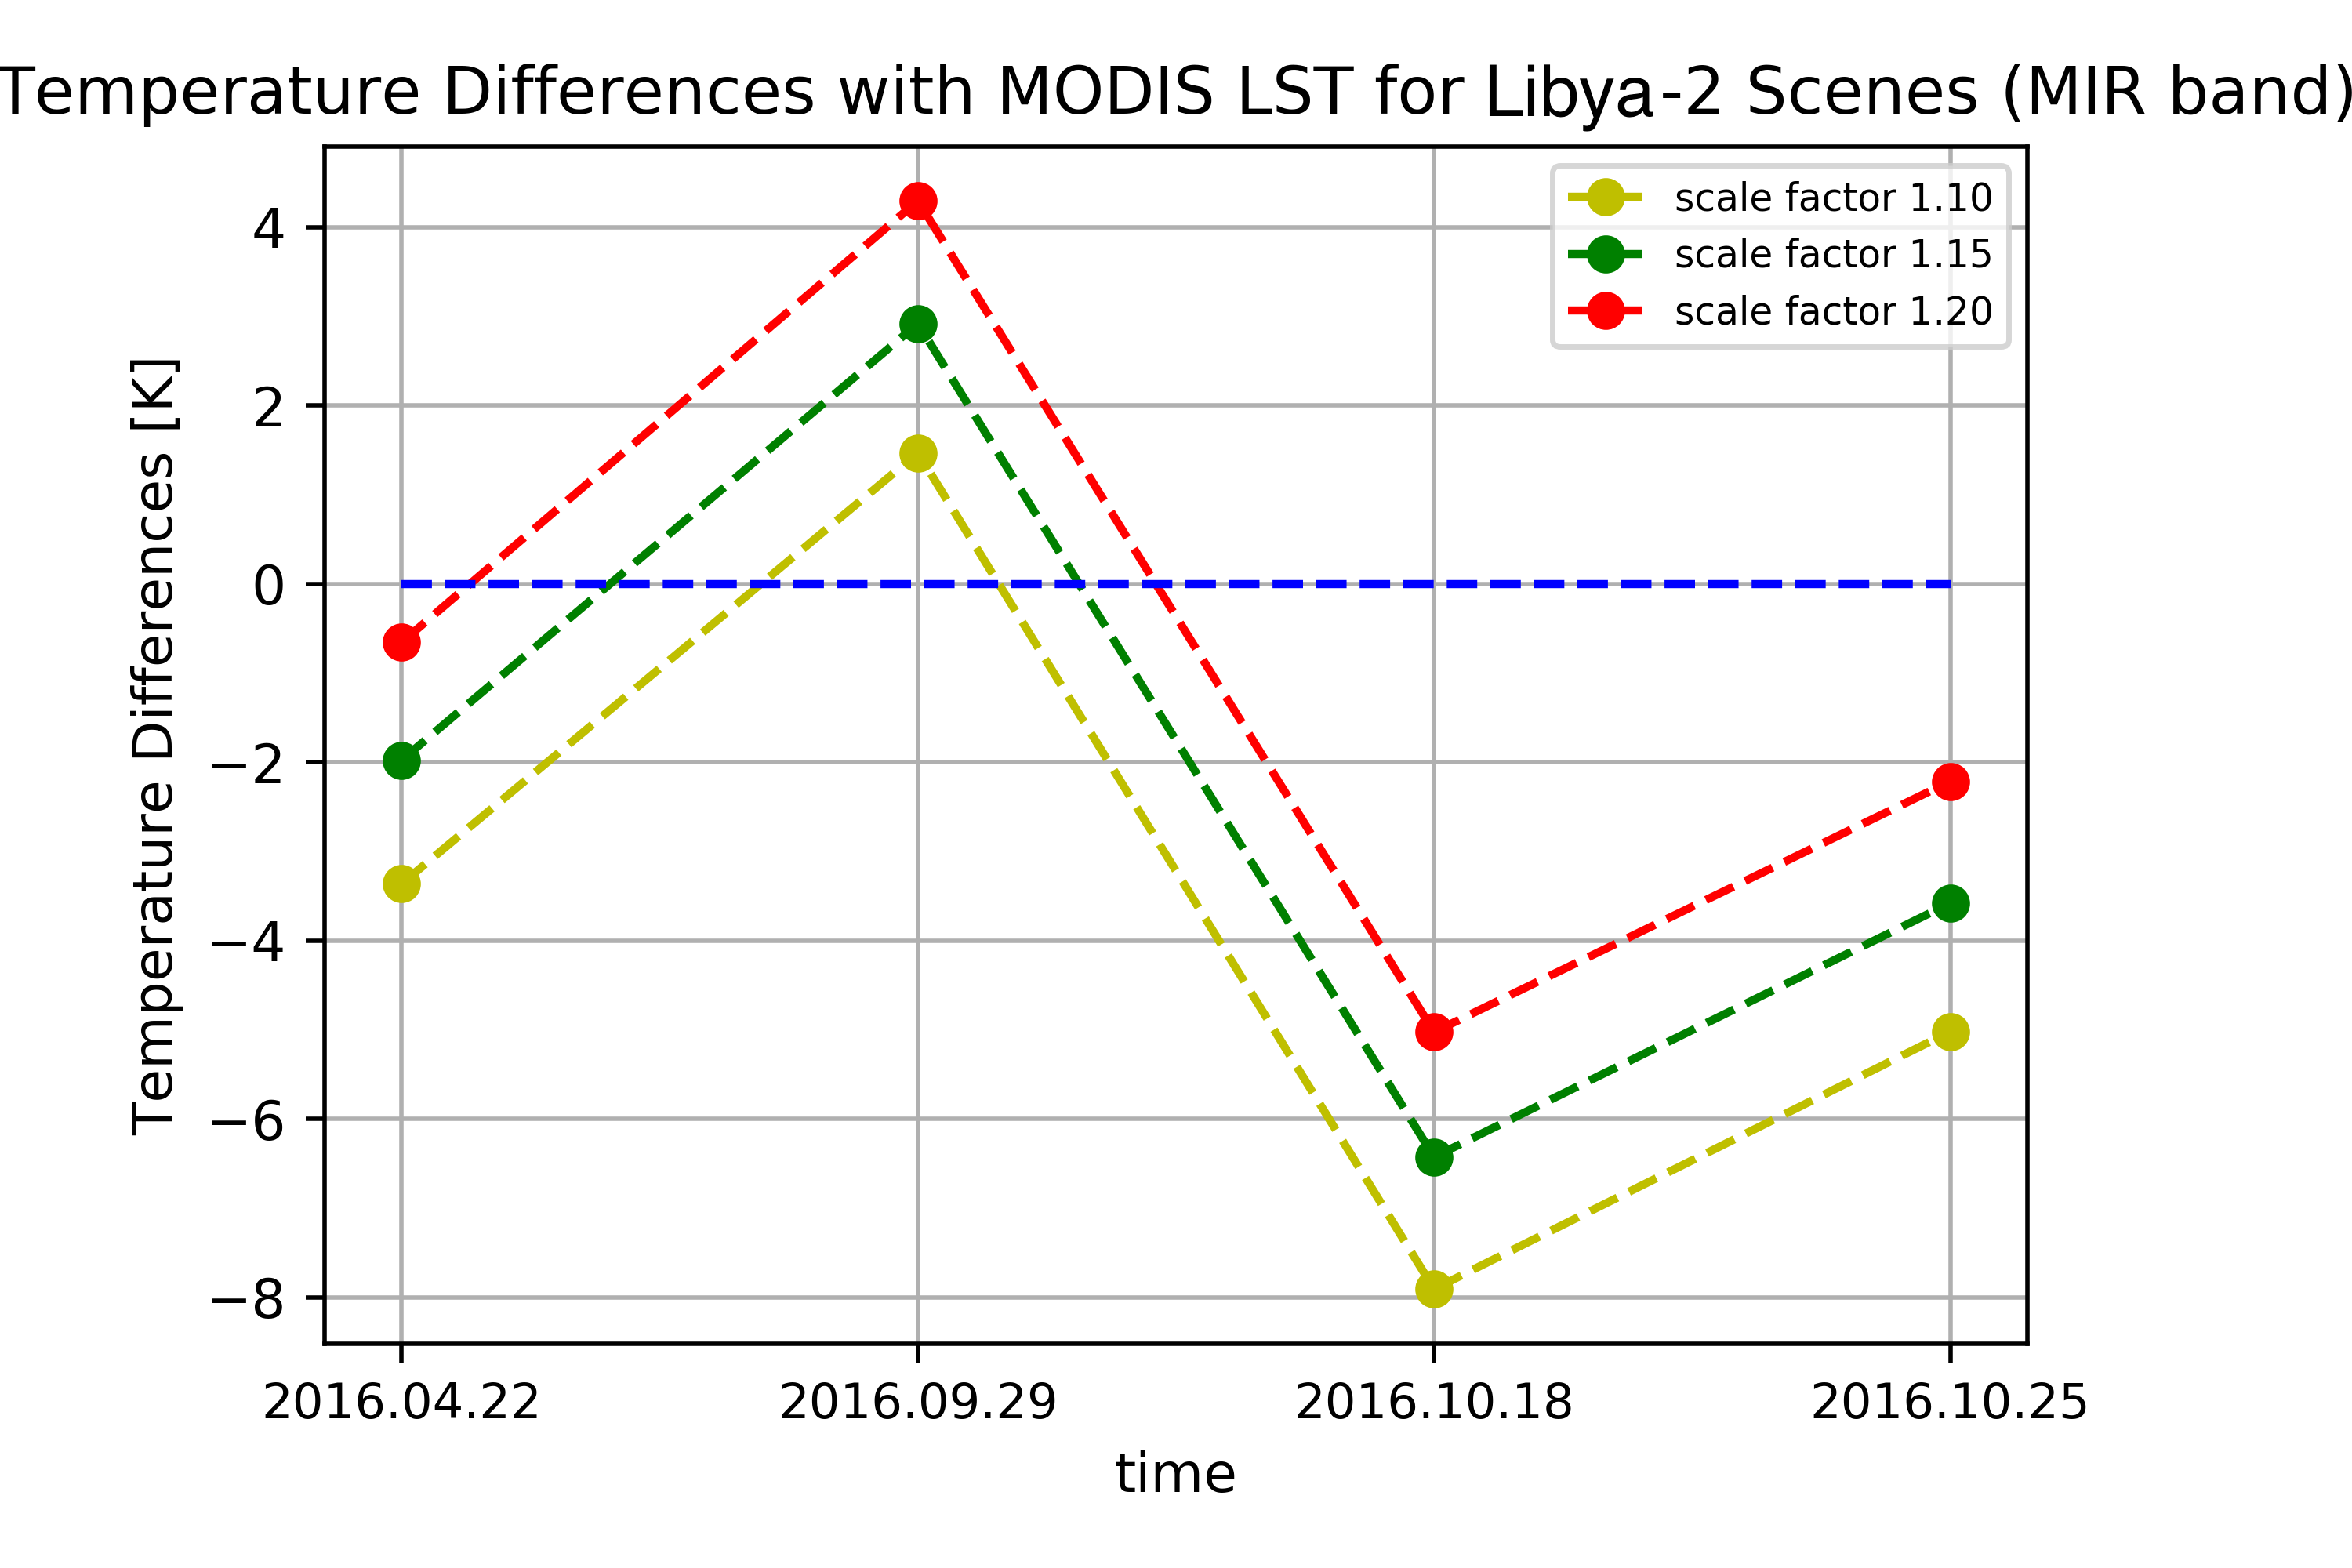
\includegraphics[width = 0.8\linewidth]{lls_test&cmp_mir.png}}
\hspace{0.5in}
\subfigure[TIR band]{
\label{fig:LST_test_tir}
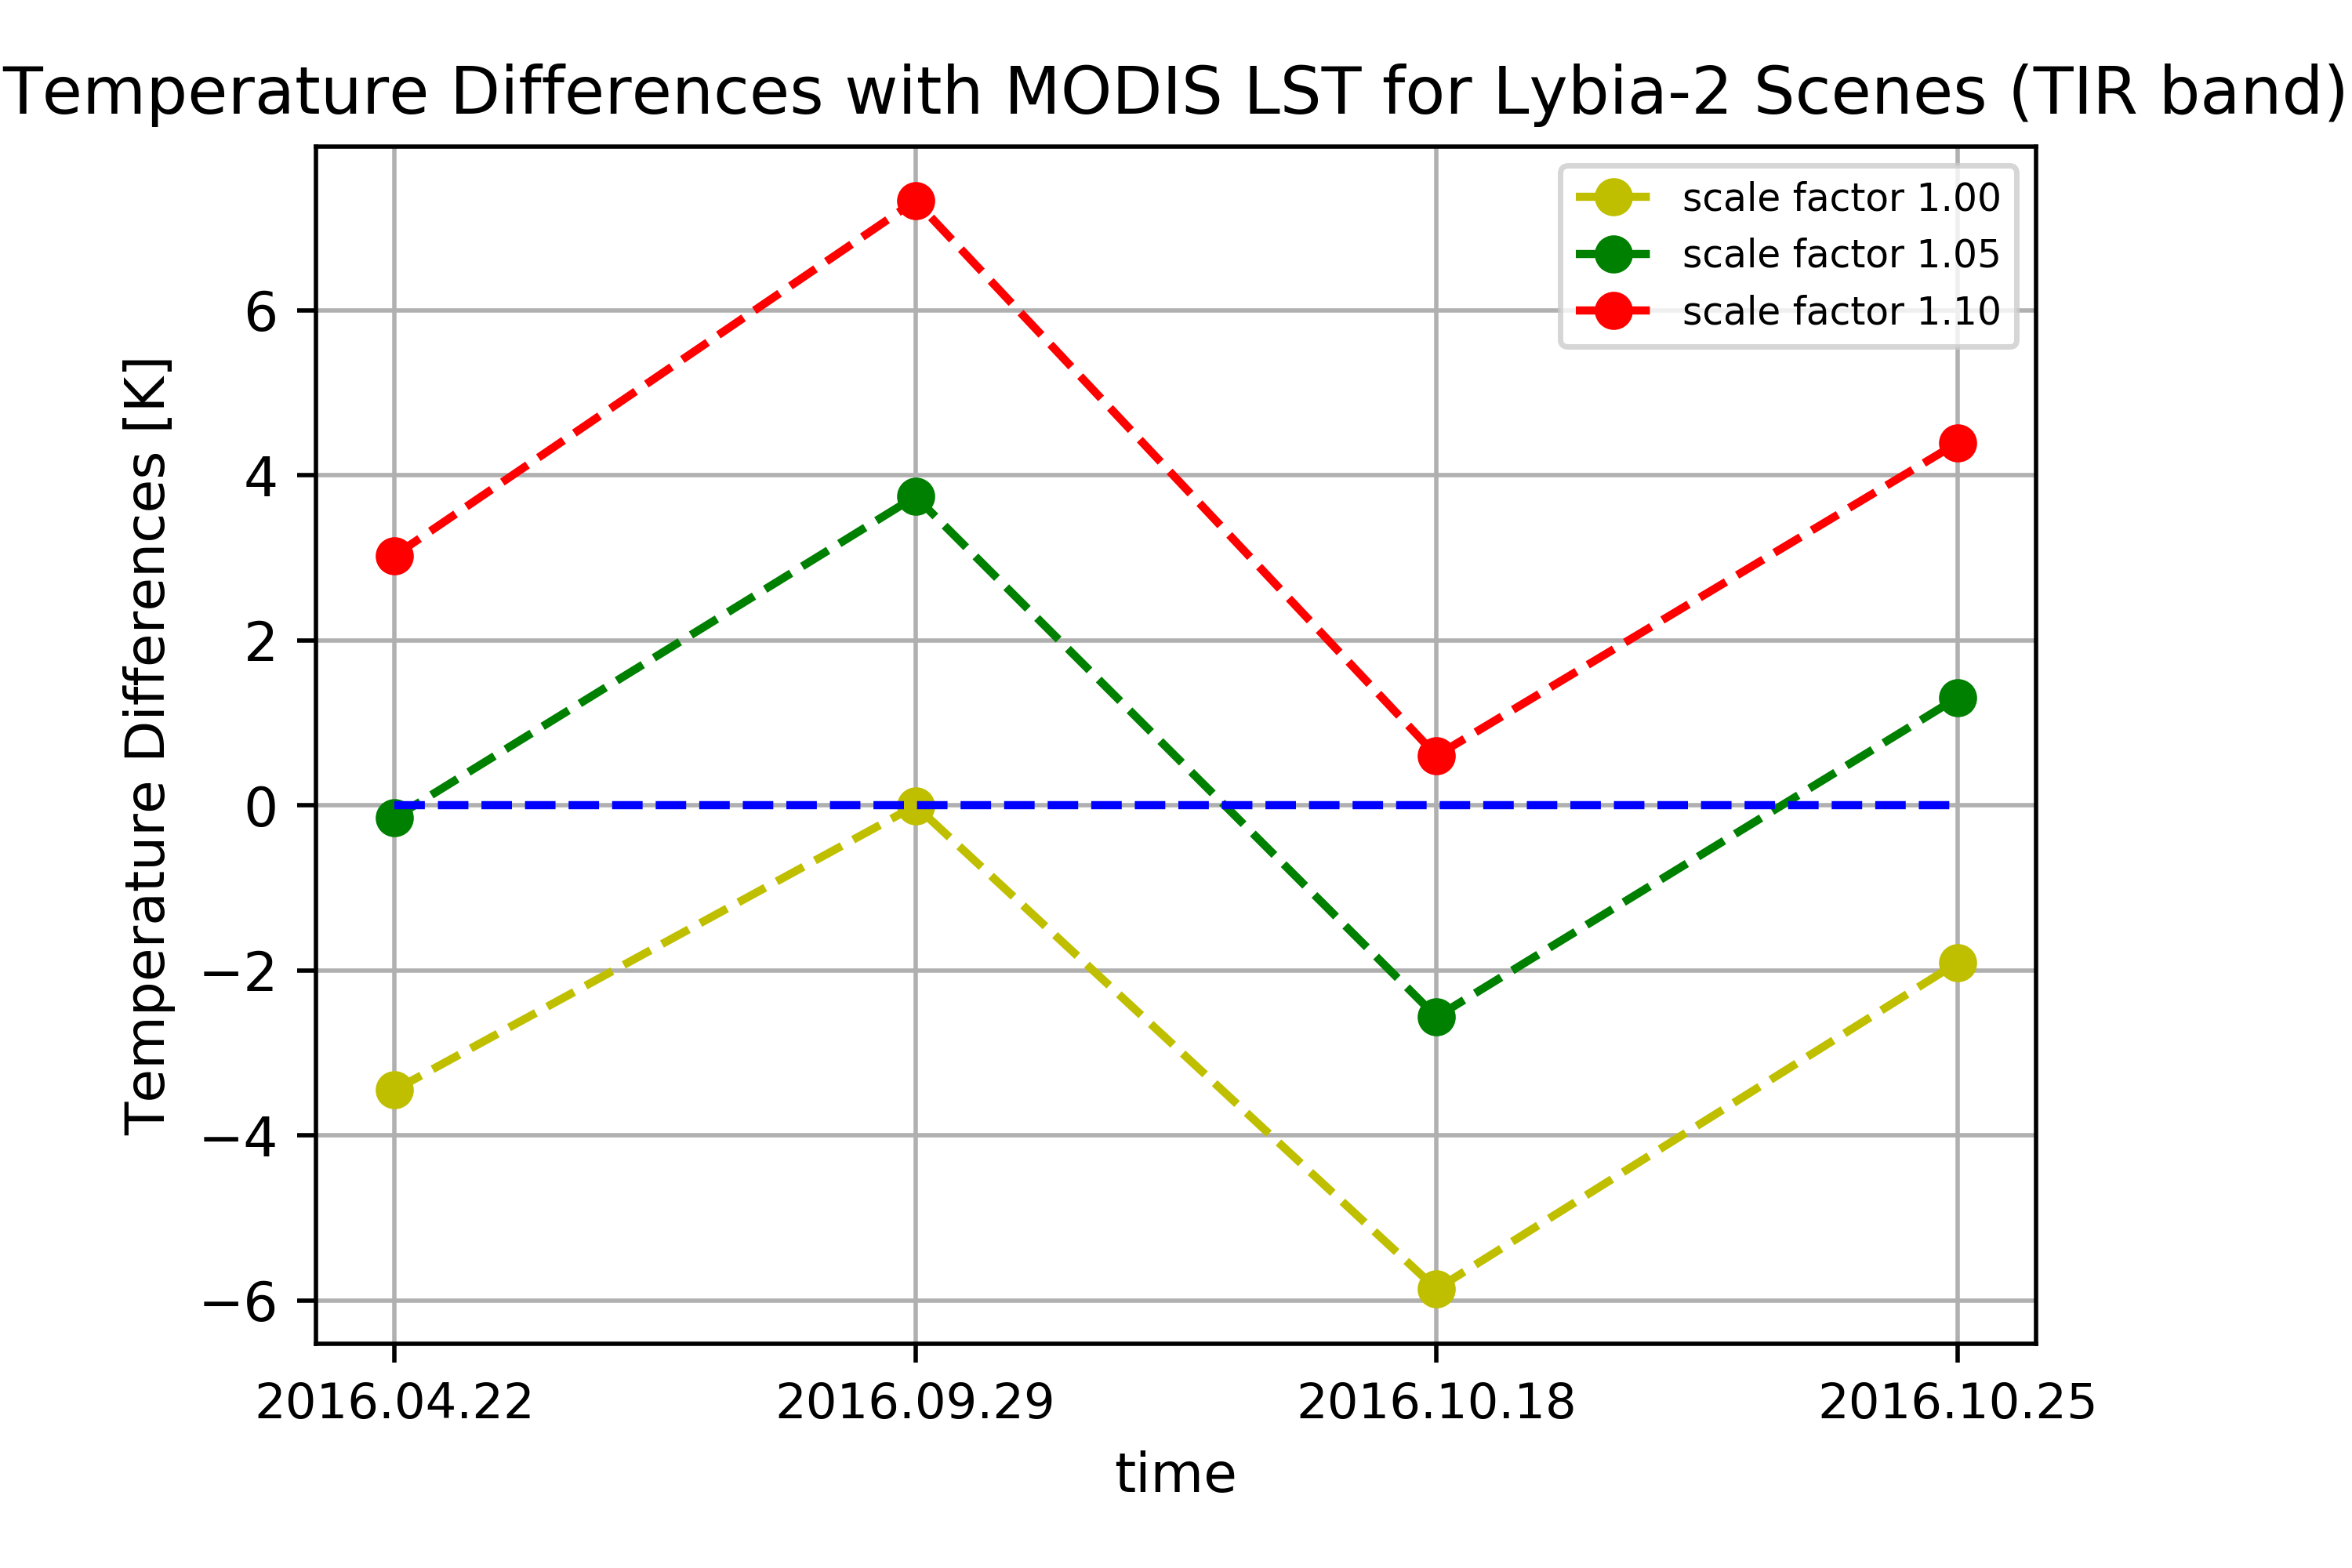
\includegraphics[width = 0.8\linewidth]{lls_test&cmp_tir.png}}
\caption{Transferability test: temperature differences between TET-1 surface temperature maps and MODIS LST.}
\label{fig:LST_test}
\end{figure}

%----------------------------------------------------------------------------------------
%	SECTION 2
%----------------------------------------------------------------------------------------

\section{Conclusion of the comparisons and calibrations}
In this chapter, the MITIP method is tested using the Etna scenes and improved by adding two key words \emph{sc1} and \emph{sc2} to calibrate the TOA radiances of the TET-1 MIR and TIR band imagery respectively. In order to find the best scale factors for the TET-1 MIR and TIR band imageries separately, the surface temperature maps in MIR band TIR band are compared with the MODIS SST firstly and then LST respectively. After all of the comparisons and tests, the optimal scale factors for TET-1 MIR and TIR band imageries are chosen as 1.15 and 1.05 respectively. Both of the scale factors performs well in both space and time domain. Later, the MITIP method will be applied to several high-temperature events scenes with the determined scale factors.\\